%!TEX encoding = UTF-8 Unicode
% ================================================================================
\documentclass[
	fontsize=12pt,
	headings=small,
	parskip=half,           % Ersetzt manuelles Setzen von parskip/parindent.
	bibliography=totoc,
	numbers=noenddot,       % Entfernt den letzten Punkt der Kapitelnummern.
	open=any,               % Kapitel kann auf jeder Seite beginnen.
%	final                   % Entfernt alle todonotes und den Entwurfstempel.
]{scrreprt}
% ================================================================================
%!TEX encoding = UTF-8 Unicode
%!TEX root = hinweiseabschlussarbeit.tex

% Kodierung, Sprache, Patches {{{
\usepackage[T1]{fontenc}    % Ausgabekodierung; ermöglicht Akzente und Umlaute
                            %  sowie korrekte Silbentrennung.
%\usepackage[utf8]{inputenc} % Erlaubt die direkte Eingabe spezieller Zeichen;
                            %  utf8 muss die Eingabekodierung des Editors sein.
\usepackage[ngerman]{babel} % Deutsche Sprachanpassungen (z.B. Überschriften).
\usepackage{microtype}      % Optimale Randausrichtung und Skalierung.
\usepackage[
    autostyle,
    ]{csquotes}             % Korrekte Anführungszeichen in der Literaturliste.
%\usepackage{fixltx2e}      % Patches fuer LaTeX2e - seit 2015 nicht mehr nötig
\usepackage{scrhack}        % Verhindert Warnungen mit älteren Paketen.
\usepackage[
  newcommands
]{ragged2e}                 % Verbesserte \ragged...Befehle
\PassOptionsToPackage{
  hyphens
}{url}                      % Sorgt für URL-Umbrüche in Fußzeilen u. Literatur
% }}}

% Schriftarten {{{
\usepackage{mathptmx}       % Times; modifies the default serif and math fonts
\usepackage[scaled=.92]{helvet}% modifies the sans serif font
\usepackage{courier}        % modifies the monospace font
% }}}

% Biblatex {{{
\usepackage[
    style=alphabetic,
    backend=biber,
    %backref=true
    ]{biblatex}             % Biblatex mit alphabetischem Style und biber.
\bibliography{\jobname.bib} % Dateiname der bib-Datei.
\DeclareFieldFormat*{title}{
    \mkbibemph{#1}}         % Make titles italics
% }}}

% Dokument- und Texteinstellungen {{{
\usepackage[
    a4paper,
    margin=2.54cm,
    marginparwidth=2.0cm,
    footskip=1.0cm
    ]{geometry}             % Ersetzt 'a4wide'.
\clubpenalty=10000          % Keine Einzelzeile am Beginn eines Absatzes
                            %  (Schusterjungen).
\widowpenalty=10000         % Keine Einzelzeile am Ende eines Absatzes
\displaywidowpenalty=10000  %  (Hurenkinder).
\usepackage{floatrow}       % Zentriert alle Floats
\usepackage{ifdraft}        % Ermöglicht \ifoptionfinal{true}{false}
\pagestyle{plain}           % keine Kopfzeilen
% \sloppy                    % großzügige Formatierungsweise
\deffootnote{1em}{1em}{
  \thefootnotemark.\ }      % Verbessert Layout mehrzeiliger Fußnoten
\ifdefined\chapterformat
	\renewcommand*{\chapterformat}{% Hübscht Kapitelüberschrift mit senkrechtem 
		\thechapter\enskip%          grauen Balken zwischen Nummer und Text auf
		\textcolor{gray!50}{\rule[-\dp\strutbox]{2pt}{\baselineskip}}\enskip
	}
\fi
%\setkomafont{disposition}{\normalcolor\bfseries} % Aus der KOMA-Skript-Anleitung: „Mit dieser Änderung verzichten Sie darauf, für alle Gliederungsebenen serifenlose Schrift voreinzustellen“

\makeatletter
\AtBeginDocument{%
    \hypersetup{%
        pdftitle = {\@title},
        pdfauthor  = \@author,
    }
}
\makeatother
% }}}

% Weitere Pakete {{{
\usepackage{graphicx}       % Einfügen von Graphiken.
\usepackage{tabu}           % Einfügen von Tabellen.
\usepackage{multirow}       % Tabellenzeilen zusammenfassen.
\usepackage{multicol}       % Tabellenspalten zusammenfassen.
\usepackage{booktabs}       % Schönere Tabellen (\toprule\midrule\bottomrule).
\usepackage[nocut]{thmbox}  % Theorembox bspw. für Angreifermodell.
\usepackage{amsmath}        % Erweiterte Handhabung mathematischer Formeln.
\usepackage{amssymb}        % Erweiterte mathematische Symbole.
\usepackage{rotating}
\usepackage[
    printonlyused
    ]{acronym}              % Abkürzungsverzeichnis
\usepackage[
    colorinlistoftodos,
    textsize=tiny,          % Notizen und TODOs - mit der todonotes.sty von
    \ifoptionfinal{disable}{}%  Benjamin Kellermann ist das Package "changebar"
    ]{todonotes}            %  bereits integriert.
\usepackage[
    breaklinks,
    hidelinks,
    pdfdisplaydoctitle,
    pdfpagemode = {UseOutlines},
    pdfpagelabels,
    ]{hyperref}             % Sprungmarken im PDF. Lädt das URL-Paket.
    \urlstyle{rm}           % Entfernt die Formattierung von URLs.
%\usepackage{breakurl}
%\def\UrlBreaks{\do\/\do-}
\usepackage{listings}       % Spezielle Umgebung für Quelltextformatierung.
    \lstset{                
        language=C,
        breaklines=true,
        breakatwhitespace=true,
        frame=l,            % Linie links: l, doppelt: L
		framerule=2.5pt,    % Dicke der Linie
		rulecolor=\color{gray},% Farbe der Linie
        captionpos=b,
        xleftmargin=6ex,
        tabsize=4,
        numbers=left,
        numberstyle=\ttfamily\footnotesize,
        basicstyle=\ttfamily\footnotesize,
        keywordstyle=\bfseries\color{green!50!black},
        commentstyle=\itshape\color{magenta!90!black},
        identifierstyle=\ttfamily,
        stringstyle=\color{orange!90!black},
        showstringspaces=false,
        }
%\usepackage{filecontents}  % Direktes Einfügen von Dateiinhalt. Wird hier für
                            %  die Verwendung einer .bib-Datei in dieser .tex-
                            %  Datei benötigt.
% }}}
% \usepackage{parskip}

% \usepackage[pdftex]{graphicx}

\usepackage{colortbl}
\usepackage{xcolor}
\usepackage{soul}

\definecolor{uhhred}{cmyk}{0,100,100,0}
\addbibresource{main.bib}

\begin{document}

\title{Privatsphärewahrendes Anreiz- und Betrugserkennungssystem im\\ Datentreuhandmodell}
\author{Knut Hoffmeister}

\newgeometry{centering,left=2cm,right=2cm,top=2cm,bottom=2cm}
\begin{titlepage}

\includegraphics[width=6.8cm]{up-uhh-logo-u-2010-u-farbe-u-rgb.pdf}
\begin{center}
    \vfill
    \Large Bachelorarbeit
    \vfill
    \makeatletter
    {\Large\textsf{\textbf{\@title}}}
    \makeatother
    \vfill
    vorgelegt von
    \par\bigskip
    \makeatletter
    {\@author}
    \makeatother
    \par
    Matrikelnummer 7509085 \par
    Studiengang Software System Entwicklung
    \vfill
    MIN-Fakultät \par
    Fachbereich Informatik
    \vfill
    \makeatletter
    eingereicht am {\@date}
    \makeatother
    \vfill
    Erstgutachter: Mathias Fischer\\
    Zweigutachter: Kevin Röbert
\end{center}
\ifoptionfinal{}{
    \begin{tikzpicture}[remember picture, overlay]
        \node[draw, red, font=\ttfamily\bfseries\Large, xshift=30mm, yshift=238mm, rotate=340, text centered, text width=6cm, very thick, rounded corners=4mm] at (current page.south) {Entwurf vom \today};
    \end{tikzpicture}
}
\end{titlepage}

\restoregeometry

\tableofcontents


\chapter*{Abstract}


%==================================================================================================


\chapter{Einleitung}
%``Die Bedeutung der Datenökonomie für die Entwicklung der Wirtschaftsleistung in Deutschland und Europa ist unbestritten`` \cite{falck2020rohstoff}\\
\label{chap:intro}
In der heutigen Zeit wird der fachgerechte Umgang mit Daten jeglicher Form zunehmend wichtiger. Viele der großen Player wie Facebook oder Google machen ihr Hauptgeschäft mit dem Verwenden von Nutzerdaten zu gewerblichen Zwecken, wie beispielsweise Targeted Ads \cite{facebookad,googlead}. Und obwohl das Misstrauen eines Nutzers, gegenüber solch einem großen Unternehmen  berechtigt ist, benötigen diese die gesammelten Daten auch dazu, neue Technologien zu entwickeln. Jedoch hat der Nutzer, der diese Daten generiert, meist keinen Einblick darin, wer seine Daten verwendet und wofür diese zum Einsatz kommen. Ein potenzieller Lösungsansatz für dieses Problem ist die Verwendung von Datentreuhändersystemen. In einem Datentreuhändersystem kann ein datengenerierender Endnutzer seine Daten verschlüsselt bei einem Treuhänder lagern. Zum anderen ist der Treuhänder ein Mediator zwischen dem Endnutzer und einem Unternehmen, das an den Daten interessiert ist. Möchte nun ein Unternehmen die Daten für ihre Zwecke verwenden, so kann dieses bei dem Treuhänder Daten anfordern. Daraufhin kontaktiert der Treuhänder den Nutzer von dem die Daten stammen und fragt diesen nach seiner Zustimmung. So kann der Nutzer genau einsehen, wer seine Daten verwenden möchte und kann unerwünschte Benutzung unterbinden. Das Ziel liegt hierbei vor allem darin den Nutzer und seine Privatsphäre so gut wie möglich zu schützen.

In dieser Bachelorarbeit sollen -- um die Motivation zur Benutzung eines Datentreuhänder zu erhöhen -- zwei Forschungsfragen beantwortet werden: Wie kann ein privatsphäreschützender Anreiz zur Benutzung eines Datentreuhändermodells geschaffen werden? Und: Wie kann dieser Anreiz gegen Missbrauch geschützt werden? Aktuell ist der einzige Anreiz zur Benutzung eines Datentreuhändermodells für den Nutzer der Schutz der Privatsphäre durch die Kommunikation über den Treuhänder. Um einen weiteren Anreiz zu bieten, soll hier ein Ansatz vorgestellt werden, der den Datengebenden für seine zur Verfügung gestellten Daten angemessen entlohnt. Dies geschieht durch eine Transaktion von dem Datennutzenden an den Datengebenden, die trotz des Austausches von Zahlungsinformationen, die Privatsphäre des Datengebenden und dessen Identität so weit wie möglich schützt. Hierfür könnte beispielsweise eine leicht erweiterte Version des GNU Taler Zahlungssystem verwendet werden (siehe Abschnitt \ref{subsec:gnu}), um den Zahlungsverkehr zwischen den Parteien zu ermöglichen. Um dieses System vor Missbrauch zu schützen, wird ein Reputationssystem eingesetzt um zu verhindern, dass ein Datengebender wertlose Daten oder qualitativ niedrigwertige Daten, in großer Masse bereitstellen kann, um so das System auszunutzen. Es soll einerseits -- gleich dem Bezahlvorgang -- die Identität des Datengebenden schützen. Gleichzeitig soll es den Datennutzenden -- der die Bewertung ausstellt -- davon abhalten, das System durch mehrfaches Bewerten auszunutzen. Auch Betrugsversuche des Datengebenden sind nicht zu vernachlässigen, wie beispielsweise die Neuanmeldung eines Nutzers mit schlechter Reputation, um diesen Wert zurückzusetzen.

Dafür wird in dieser Arbeit der aktuelle Stand der Forschung in dem vorliegenden Kontext evaluiert und geprüft, was bereits anwendbar und wo noch Lücken zur gewünschten Verwendung bestehen. Mit den gesammelten Forschungsergebnissen wird daraufhin ein Konzept präsentiert, um das gerade genannte Ziel in das Treuhändermodell zu integrieren. Dieses Konzept wird desweiteren in ein bestehendes Treuhändersystem eingebaut, um konkrete Vergleichsgrundlagen zu erhalten. Bei dem hierfür vorgesehenen System handelt es sich um das Tresor-Projekt der Universität Hamburg \cite{TRESOR}.


%==================================================================================================


\chapter{Grundlagen}
\label{chap:basics}
Die zunehmende Digitalisierung unseres Alltags ist unbestreitbar \cite{dt-digitalisierung-stat}. Viele der täglichen Aktivitäten basieren stark darauf. Sei es den schnellsten Weg zur Arbeit mit Google Maps zu finden, das kontaktlose Bezahlen an der Kasse mit GooglePay oder Applepay, die Benutzung von Social Media zur Unterhaltung oder der Onlinehandel über Anbieter wie Amazon. Sie alle liefern Komfort, der durch die zunehmende Verwendung von Computern ermöglicht wird, die im Hintergrund Unmengen an Daten für ihre Berechnungen verwenden. Diese Daten stammen meist von den Benutzern selbst. beispielsweise die Standortdaten für die Berechnung potenzieller Staus im Straßennetz \cite{dt-googlemaps-staus} oder die Unterhaltungsinteressen basierend auf Watchtime von bestimmten Social Media Inhalten. \\
Aufgrund des ständig wachsenden Marktes für neue Digitaltechnologien ist auch die Nachfrage nach Daten im laufe der letzten Jahre in die Höhe gestiegen. Im letzten Jahrzehnt haben die Daten, das Öl als wertvollste Ressource abgelöst. Während im Jahr 2008 die vier weltweit wertvollsten Unternehmen Ölkonzerne waren, waren es in 2018 bereits die sieben wertvollsten Unternehmen Internet- und Technologiefirmen \cite{dt-falck2020rohstoff}. 

\section{Reguläre Datenkommunikation}
In Anbetracht des hohen Wertes von Daten sind viele Unternehmen verständlicherweise mit dem Austausch der Daten zurückhaltend. Schließlich beutet eine eigene Datensammlung ein potenzielles Verkaufsgut. Laut einer Studie von Fedkenhauer et al. geben zwar viele der befragten Unternehmen an, Aktivitäten im Bereich des Datenaustausches zu betreiben, allerdings umfasst das in 83\% der Fälle den Austausch von Daten mit Kundinnen und Kunden. 53\% der Unternehmen teilen ihre Daten mit Lieferantinnen und Lieferanten. Ein noch kleinerer Anteil von 21\% teilt seine Daten mit Unternehmen aus den gleichen oder anderen Branchen und nur 15\% teilen sie mit Wettbewerbern \cite{dt-fedkenhauer2017datenaustausch}. \\\\
Aus der kapitalgetriebenen Sicht eines Unternehmens besitzt das Teilen der eigenen Daten keinen direkten Nutzen. Da ein Unternehmen seine eigene Gewinnmaximierung anstrebt, ist das Teilen von Daten eher ein Nachteil, da fremde Unternehmen mit den selbst gesammelten Daten ihre Produkte qualitativ erweitern können. Dadurch werden entweder andere Wettbewerber oder branchenfremde Unternehmen in ihrem Marktwert gefördert, was zu der Verrinnerungen des eigenen Marktanteils führt. \\
Diese protektive Herangehensweise kann allerdings auch der Gewinnmaximierung im Weg stehen. Im Fall vom direktem Tausch an Daten können beide Parteien einen Profit aus der Interaktion erwirtschaften. Die Bundesregierung selbst schreibt in \cite{dt-bundesregierung2021datenstrategie}, dass kaum Datenkooperationen zwischen staatlichen und wirtschaftlichen Akteurinnen bestehen, obwohl die staatlich gesammelten Daten eine Grundlage für wirtschaftliche Innovation sein könnten. Im Gegenzug könnten die Daten von Unternehmen dem Staat bei der Sicherstellung seines Versorgungsauftrages, der Daseinsvorsorge und der Wahrung öffentlicher Schutzgüter helfen. Dies ist eine optimale Situation für die Verwendung eines Datentreuhänders.
\section{Datentreuhänder}
\label{sec:dt}
Ein Datentreuhänder ist ein neutraler vertrauenswürdiger Vermittler von Daten eines Datengebenden zu einem Datennutzenden. Er hat selbst kein kommerzielles Interesse an der Verwertung der Daten und agiert vergleichbar zu einem Notar im Sinne des Datengebers. Seine Hauptaufgaben umfassen großteils die Kontrolle von Zugriffsrechten, das Kontrollieren von Einhaltung der Datenschutzrichtlinien, sowie das Verschlüsseln oder Anonymisieren von Datenbeständen. In speziellen Fällen kann ein Datentreuhänder auch die Auswertung von Daten vornehmen. \cite{dt-bundesregierung2021datenstrategie}\cite{dt-richter2020ddvtalk}

Da -- wie bereits angeführt -- viele Unternehmen die Weiterleitung ihrer Daten vermeiden, ist unter der Annahme eines etablierten Datentreuhänders ein deutlich größerer Datenbestand verfügbar. Bereits heute -- vor einer großen Etablierung von Datentreuhänder -- verspricht das Konzept einige gesellschaftliche Vorteile: \cite{dt-richter2020ddvtalk}
\begin{enumerate}
    \item Dadurch können Datenbestände besser vernetzt werden und Zusammenhänge hergestellt werden, die zu Innovationen führen.
    \item Der Wettbewerb unter Firmen wird gestärkt, weil mit besser zugänglichen Daten auch kleinere Unternehmen, die kein Datenmonopol besitzen, ihre Produkte aufwerten können.
    \item Der individuelle Endnutzer erhält mehr Kontrolle und Transparenz über die Speicherung und Verwendung seiner Daten.
\end{enumerate}

Allerdings ist das Verständnis eines Datentreuhänders nicht eindeutig. Jürgen Kühling beschreibt den Datentreuhänder als ``ein schillerndes Wesen. Jeder kennt ihn, jeder setzt ganz eigene Hoffnungen in ihn – und jeder stellt sich doch etwas anderes unter ihm vor`` \cite{dt-kuhling2021datentreuhander}. Obwohl die Technologie eines Datentreuhänders bereits seit Jahren existiert und verwendet wird \cite{dt-hardinges2018data} ist es bisher nicht gelungen, eine konkret allumfassende Definition für die Technologie zu finden.

\subsection{Definition}
Die allgemeingültigste Definition stammt aus der Rechtswissenschaft und bezieht sich auf die Treuhandschaft im Allgemeinen. ``\textit{[Treuhandschaften sind ein] Rechtsverhältnis, bei dem eine natürliche oder juristische Person (Treugeber) einer zweiten Person (Treuhänder) ein Recht unter der Bedingung überträgt, von diesem Recht nicht zum eigenen Vorteil Gebrauch zu machen. [...] Gemeinsames Charakteristikum ist die Uneigennützigkeit und Vertrauenswürdigkeit bei der Wahrnehmung fremder Interessen bzw. die uneigennützige Ausübung von amtlichen Befugnissen.}''\cite{dt-beeck2013treuhandschaft}. Diese Treuhandschaft wurde in der Vergangenheit verwendet, um beispielsweise Ländereien zu verwalten und im Namen einer lokalen Gemeinschaft Entscheidung zu treffen. \cite{dt-hardinges2018data}. In dem Fall eines Datentreuhänders bedeutet dies konkret, dass eine Datengebende Person beim Bereitstellen ihrer Daten den Datentreuhänder dazu ermächtigt, über diese Daten zu verfügen. Darunter fällt unter anderen auch die Weitergabe der Daten, solange die im Sinne des Datengebers ist. 

\subsection{Verschieden Modelle}
Insgesamt lassen sich alle bis zum heutigen Zeitpunkt in Betrieb genommenen oder geplanten Datentreuhandsysteme wie folgt kategorisieren: Zum einen besteht die Einteilung in Customer to Business (C2B) oder Business to Business (B2B) Systeme und zum anderen die risikobasierte Einteilung nach Zentralen/Dezentraler Datenspeicherung und Freiwilliger/Verpflichtender Nutzung. (siehe Abbildung \ref{fig:dt-risikoeinteilug})

Die Unterscheidung zwischen Customer to Business (C2B) und Business to Business (B2B) Datentreuhändern basiert ausschließlich auf den interagierenden Parteien. Im Falle einer B2B Interaktion kommunizieren zwei Unternehmen die vorhandenen Daten miteinander. In diesem Fall kommt es häufig vor, dass eines der Unternehmen durch eine staatliche Behörde dargestellt wird \todo{proof}. Bei den gespeicherten Daten handelt es sich meist um personenbezogene Daten. Aufgrund dessen befassen sich B2B Datentreuhänder häufig mit der Pseudonymisierung und der Verwaltung der bereitgestellten Daten \todo{proof}. Sie sind unter anderem im Gesundheitswesen häufig vertreten. \cite{dt-blankertz2020datentreuhandmodelle}
C2B Systeme umfassen solche, bei denen ein Endnutzer die Daten generiert und diese an ein Unternehmen zur weiteren Benutzung freigibt. Ihre Aufgabe ist hauptsächlich die Unterstützung des Nutzers bei der gerechten Weiterverarbeitung seiner Daten. \cite{dt-blankertz2020datentreuhandmodelle} Hier sind dementsprechend die Pseudonymisierung der Daten sowie die Einhaltung von Datenschutzrechtlinien und einheitlicher Standards die Hauptziele des Datentreuhänders.

Des Weiteren lassen sich Datentreuhandsysteme anhand ihrer Datenspeicherung sowie Nutzung kategorisieren und Risikotechnisch bewerten. Die zentrale Speicherung der Daten bietet einige Vorteile für den Treuhänder. Sie ermöglicht es Daten vorzuverarbeiten, zu analysieren und Datenverarbeitende von dem direkten Zugang der Daten auszuschließen. Allerdings birgt die zentrale Datenspeicherung ein enormes Risiko der Datensicherheit, da hier ein Single Point of Failure entsteht. Bei einem Angriff auf einen solchen Datentreuhänder fällt es einem Angreifer somit leichter eine große Menge an Daten zu stehlen. Bei einer dezentralen Speicherung werden die Daten direkt bei den Datengebenden gelagert, was die Auswirkungen eines Angriffes erheblich senken kann. 
%Aus diesem Grund bietet eine dezentrale Datenspeicherung mehr Sicherheit vor Diebstahl. Sie zieht allerdings auch eine eingeschränkte Verarbeitung und Analyse der Daten mit sich und erhöht die Komplexität der Verwaltung.
\\

Es besteht eine weitere Unterteilung in Datentreuhandsysteme, dessen Benutzung freiwillig oder verpflichtend ist. Dabei fällt der größte Anteil an Systemen unter die freiwillige Benutzung \todo{proof}. Es gibt jedoch auch Szenarien, in denen die Verwendung einer Datentreuhand verpflichtend ist. Ein Beispiel hierfür wäre das Krebs- und Transplantationsregister aus dem medizinischen Bereich. Das Risiko steigt bei verpflichtenden Systemen, da sie meist einen wichtigen Bestandteil der Kommunikation ausmachen, der nicht umgangen werden kann. Somit sind die potenziellen Schäden, die bei einem Angriff entstehen können, höher als in einem freiwilligen System.

\begin{figure}
    \centering
    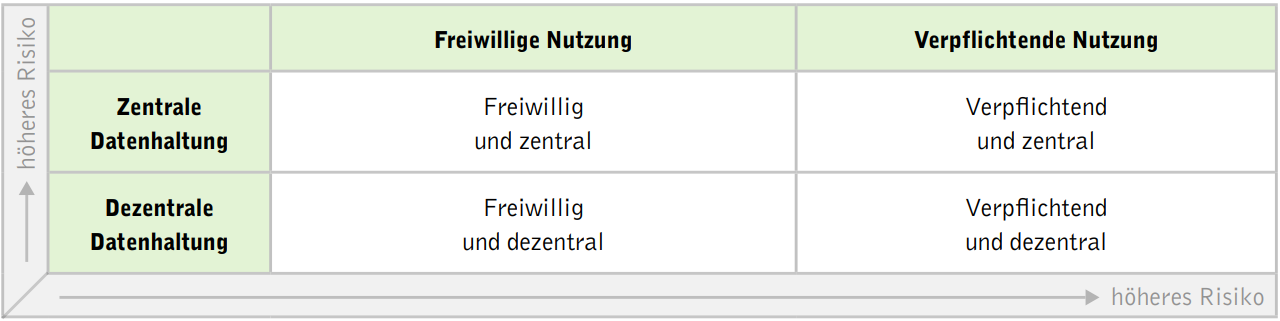
\includegraphics[width=0.9\textwidth]{DT-RisikoEinteilung.png}
    \caption{Risikobasierte Unterscheidung von Datentreuhandmodellen \cite{dt-blankertz2021neue}}
    \label{fig:dt-risikoeinteilug}
\end{figure}

\section{Anwendungsfälle}
\label{sec:dt-usecases}
Das mögliche Spektrum an Anwendungsfällen ist denkbar breit. In beinahe jedem Bereich, der eine große Menge an Daten benötigt oder verwaltet ist die Verwendung eines Datentreuhänders angedacht \cite{dt-blankertz2021regulierung,dt-blankertz2021neue, dt-bundesdruckereiDatentreuhänder}. Beispiele dafür sind:
\begin{itemize}
    \item \textbf{Patientendaten.} Der Datentreuhänder sorgt für eine Pseudonymisierung von Patientendaten zur Bereitstellung an Forschungseinrichtungen. Hierbei behält der Patient die Kontrolle über seine Daten und kann selbst entscheiden, mit wem seine Daten geteilt werden.
    \item \textbf{Autonomes Fahren.} Beim autonomen Fahren werden enorm viele Daten generiert, die seit 2017 per Gesetz gespeichert werden müssen \cite{dt-bundesdruckereiDatentreuhänder}. Leider ist die Zugehörigkeit der Daten rechtlich weder dem Autohersteller noch dem Autoinhaber zuzuschreiben \cite{dt-richter2020ddvtalk}. An dieser Stelle kann ein Datentreuhänder die Kommunikation erleichtern und exklusiven Zugang von beispielsweise Versicherungen oder Automobilkonzernen ausschließen.
    \item \textbf{E-Government.} Durch die Verwendung eines Datentreuhänders können bei der behördlichen Verwaltung von Bürgerdaten große Fortschritte erzielt werden. Unter anderem müssen notwendige Informationen aus anderen Registern für Verwaltungsvorgänge nicht mehr vom Bürger bereitgestellt werden. Der Bürger gibt lediglich seine Einwilligung zum Abruf der Daten zu Beginn des Verwaltungsvorgangs. Auf diese Weise können Verwaltungsvorgänge erheblich effizienter Ablaufen.
    \item \textbf{KI-Datenpools.} Eines der größten Probleme bei Entwicklung von KI-Software ist der Zugang zu einer ausreichend großen Menge an Trainingsdaten. Ein Datentreuhänder kann solche Daten, die zur Verwendung für KI-Training freigegeben wurden, sammeln und pseudonymisiert an mehrere Interessierte verteilen. Dadurch entsteht ein einheitlicher Zugang zu Trainingsdaten der gleichzeitig nur freigegebene Daten beinhaltet und so rechtlichen Streit über die Urheberschaft aus dem Weg geht.
    \item \textbf{Industrie.} In der Industrie besteht eine hohe Abhängigkeit von Warenbewegungen, seien es in Lieferketten, Logistik oder Handel. Durch die Verwendung eines Datentreuhänders können diese Informationen pseudonymisiert an Warenempfänger weitergegeben werden. Vor allem in diesem Bereich besteht durch die Zusammentragung an Lieferinformationen in Kombination mit Algorithmen der Graphentheorie ein großes Innovationspotential.
    \item \textbf{PIMS.} Personal Information Management Systeme befassen sich grundsätzlich mit der Wahrung von personenbezogenen Daten und bieten ihren Nutzern mehr Kontrolle über diese.  Datentreuhänder sind für solche Systeme vor allem von Vorteil, da sie im Umgang mit personenbezogenen Daten dem Nutzer wieder die Kontrollen über seine Daten zurückgeben.
\end{itemize}

Der erste Datentreuhänder entstand bereits im Jahre 2006 in England. Das Thema Datentreuhänder wurde in den letzten Jahren immer mehr zum Trend \cite{dt-richter2020ddvtalk}. Die ``UK Biobank`` ist eine biomedizinische Datenbank, die sowohl medizinische Daten als auch biologische Proben von einer halben Millionen Teilnehmer aus Großbritannien speichert \cite{dt-hardinges2018data}. Die gespeicherten Daten sind pseudonymisiert und werden ausschließlich an Forscher im Feld der Medizin weitergegeben, was die UK Biobank zu einem Paradebeispiel für einen Patientendatentreuhänder macht.


\section{Bestehende Anreize}
Insgesamt bringt die Verwendung eines Datentreuhänders keine direkten Nachteile mit sich. Wenn Daten ohnehin geteilt werden oder werden müssen, behält der Nutzer bei der Speicherung der Daten über einen Datentreuhänder mehr Kontrolle über die Verwendung seiner geteilten Daten, als im Vergleich mit dem direkten Teilen mit Unternehmen. Durch den Datentreuhänder wird ihm ermöglicht, zu einem beliebigen Zeitpunkt das weitere Teilen seiner Informationen einzustellen. Vermutlich teilen deswegen Privatpersonen ihre Daten lieber mit Datentreuhändern als auf direktem Weg. \cite{dt-tresor24study}

Allerdings gibt es nur wenige Vorteile, die die freiwillige Benutzung eines Datentreuhänders reizvoll machen. Bei freiwilligen C2B Datentreuhändern liegt die Entscheidung für oder gegen die Nutzung des Treuhänders beim Nutzer. Es ist also an ihm abzuwägen, ob die Verwendung ausreichend Vorteile liefert. Im Fall von PIMS-Treuhändern wird die Verwendung von manchen als erstrebenswert angesehen, da der Nutzer mehr Kontrolle über die Verbreitung von persönlichen Daten erhält und selbst entscheiden kann, mit wem diese geteilt werden. Die Erkenntnisse von Jai et al. \cite{dt-jai2016privacy} zeigen hingegen, dass vor allem jüngere Erwachsene weniger Wert auf den Schutz ihrer persönlichen Daten legen.

Direkte Anreize zur Verwendung einer solchen Software sind bisher kaum präsent. An der Weitergabe der persönlichen Daten hat nur das Business einen konkreten Mehrwert \todo{proof}. Der Nutzer, der seine Daten freigibt, erhält keine Kompensation in irgendeiner Form. Folglich kann es für einen freiwilligen Datentreuhänder mühsam sein, neue Nutzer zu gewinnen und die Technologie als solche auszubauen.


%==================================================================================================


\chapter{Angreifermodelle und Anforderungen}
In diesem Kapitel werden zuerst die Angreifermodelle für das später entworfene Bezahl- und Reputationssytems definiert und anhand ihrer die Anforderungen für die Systeme aufgestellt.
\label{chap:req}
\section{Definition der Angreifermodelle}
Angreifermodelle sind ein in der Informationssicherheit weit verbreitetes Konzept, mit dem sich die Stärke eines Systems gegen Angriffe eines theoretischen Angreifers zeigen lässt. Ein Angreifermodell besteht aus Angreiferzielen, die ein Angreifer mit seinem Angriff erreichen möchte. Angreiferannahmen die Aussagen über die Ressourcen und das Umfeld des Angreifers aussprechen. Und Angreiferfähigkeiten welche dem Angreifer eine Liste an möglichen Angriffsmethoden zu verfügung stellen. Zusammen ergibt sich aus diesen drei Spezifikationen ein Angreifer dessen macht gerade so nicht ausreicht, damit der Angreifer sein definiertes Ziel erreicht. Eine ausführliche Erklärung von Angreifermodellen folgt in Kapitel \ref{chap:auswertung}. Hier werden fünf Angreifermodelle für die unterschiedliche Akteure der später eingeführten Systeme aufgestellt.\\

Die Angreiferfähigkeiten beschränken sich bei allen folgenden Angreifermodellen auf die Verwendung von polynomialzeit Algorithmen und das Verfügen über unbegrenzten Speicherplatz.
\begin{enumerate}
    \item \textbf{Neugierig aber ehrlicher Datentreuhänder.} Das Ziel des neugierigen Datentreuhänders ist, anhand der über ihn laufenden Kommunikation ausreichend Informationen über den Datengebenden und den Datennutzenden zu erhalten, um die Handelsbeziehungen zwischen den beiden Akteuren verfolgen zu können. Er muss sich an die im Protokoll vorgeschriebenen Schritte halten und darf nur anhand der mitgeschnittenen Nachrichten Analysen tätigen.
    \item \textbf{Bösartiger Datengebender.} Ein bösartiger Datengebender möchte das System ausnutzen und ohne (oder möglichst wenige) Daten zu teilen so  viele Coins wie möglich erhalten. Er darf vom vorgegebenen Protokoll abweichen und kann über die erhaltenen Informationen frei verfügen, sowie diese öffentlich teilen.
    \item \textbf{Bösartiger Datennutzender.} Bösartige Datennutzende zielen darauf ab, die Identität der Datengebenden über mehrere Handel zu verlinken und so ein Pseudoyn mit allen von diesem Datengebenden erhaltenen Daten zu erstellen. Zusätzlich möchte er für das Empfangen von Daten keine Coins ausgeben. Der bösaritge Datennutzende darf ebenfalls vom Protokoll abweichen und kann vorgeschriebene Berechnungswege ersetzen. Er kann Analysen anhand der mitgeschnittenen Nachrichten erstellen.
    \item \textbf{Neugierig aber ehrlicher Exchange.} In dem in den Abschnitten \ref{system:coingeneration} und \ref{system:payment} eingeführten Systemen, können Coins zum bezahlen des Datengebenden bei einem Exchange erstellt und eingelöst. Genauere Details werden in den jeweiligen Abschnitten genannt. Das Ziel des Exchanges ist, die ausgestellten Coins beim späteren einlösen wieder zu erkennen und so Schlüsse über die Beziehung zwischen Datennutzenden und Datengebenden zu ziehen. Außerdem möchte er einen Überblick darüber haben, welcher Datennutzende wie viele Coins erstellt hat und wie viele er davon bereits ausgegeben hat. Der Exchange ist in dem meisten Teilen an das Protokoll gebunden und kann nur an einer Stelle von diesem Abweichen. Er kann ebenfalls Analysen über die mitgeschnittenen Daten erstellen und probieren aus ihnen Informationenen zu gewinnen.
    \item \textbf{Außenstehender Angreifer.} Ein außenstehender Angreifer ist nicht in Kommunikation involviert, sondern möchte anhand sämtlicher übertragener Nachrichten zwischen zwei Akteuren herausfinden, wer mit wem kommuniziert und was in der Nachricht enthalten ist. Dafür kann er alle Nachrichten die innerhalb der Protokoll ausgetauscht werden mitschneiden. Er kann auch mit den empfangenen Nachrichten selbst die Kommunikation mit einem Akteur aufnehmen und sich als ein Teilnehmer der Kommunikation ausgeben.
\end{enumerate}

\section{Funktionale Anforderungen}
\label{enum:req:funktional}
\begin{enumerate}
    \item Ein Bezahlsystem ermöglicht es einem Datengebenden Geld für seine Daten zu erhalten.
    \item Ein Reputationswert gibt vor Erwerb der Daten durch den Datennutzenden eine Einschätzung über deren Qualität.
    \item Nach Erhalt von Daten muss ein Datennutzender den Datengebenden für die erhaltenen Daten bezahlen und diese Bezahlung auf Nachfrage nachweisen können.
    \item Nach Abschluss der Transaktion kann ein Datennutzender den entsprechenden Datengebenden aufgrund der Qualität der übermittelten Daten bewerten.
    \item Ein Datengebender muss eine Bewertung seiner Daten ermöglichen.
    \item Ein Datennutzender kann pro Austausch nur genau eine Bewertung für einen Datengebenden abgeben. Mehrfache Bewertungen ist nur im Fall von mehrfachem Erwerb möglich.
\end{enumerate}

\section{Nicht funktionale Anforderungen}
\label{enum:req:nichtfunktional}
\begin{enumerate}
    \item \textbf{Anonymität.} Die Identität des Datengebenden darf durch den Austausch von Zahlungsmitteln oder durch dessen Reputation nicht offengelegt werden.
    \item \textbf{Unverkettbarkeit.} Mehrere Transkationen eines Datengebenden dürfen keine Informationen über den Zusammenhang dieser aufweisen. 
    \item \textbf{Zeitsensitivität.} Der Bezahlvorgang muss in vernachlässigbarer Zeit geschehen.
    \item \textbf{Skalierbarkeit.} Die Rechenzeit des Systems soll bei linear steigender Menge an Transkationen auch mit linearem Zeitaufwand zunehmen.
    \item \textbf{Vertraulichkeit.} Die kommunizierten Daten dürfen nicht durch unbefugte Dritte ausgelesen werden können.
    \item \textbf{Integrität.} Die kommunizierten Daten dürfen nicht unbemerkt durch unbefugte Dritte verändert werden.
\end{enumerate}

\chapter{Verwandte Arbeiten}
In diesem Kaptiel werden bestehende Arbeiten vorgestellt, die eine dichte Verbindung zu dem Thema dieser Bachelorarbeit haben. Dafür wird das Produkt der Arbeit erklärt und anschließend erläutert warum diese Arbeiten in dem Umfeld eines Datentreuhänders nicht eingesetzt werden können. Die Arbeiten beziehen sich zuerst auf weitere Bezahlsystem und behandeln später Bausteine die für die Konstruktion des hier dargelegten Bezahlsystems essentiell sind.

\section{GNU Taler}
\label{subsec:gnu}
Das im Paper ``Enabling Secure Web Payments with GNU Taler`` von J. Burdges et al. eingeführte Zahlungssystem GNU Taler ist ein elektronisches Online-Zahlungssystem, das Datenschutz für Customer und Mechanismen zur steuerlichen Nachverfolgung für Merchants bietet \cite{gnu-burdges2016enabling}. Es verwendet einen Exchangeservice, um Münzen mithilfe von blinden Signaturen zwischen Nutzern und Händlern zu transferieren. Im Folgenden werden diese Münzen als Taler bezeichnet. Das System basiert auf vier übergeordneten Rollen, dessen Interaktion grob in Abbildung \ref{fig:gnu_taler_overview} skizziert ist. Der Customer möchte ein Gut oder eine Dienstleistung bei dem Merchant erwerben und bezahlt diesen dafür mit Talern, die er beim Exchange erworben hat. Der Merchant kann die erhaltenen Taler wieder beim Exchange für herkömmliche Währungen eintauschen. Ein Auditor überprüft währenddessen die Liquidität des Exchange, um sicherzustellen, dass dieser auch bei Datenverlust von Talern noch in der Lage ist, allen Beteiligten Auszahlungen zu ermöglichen.

\begin{figure}[H]
    \centering
    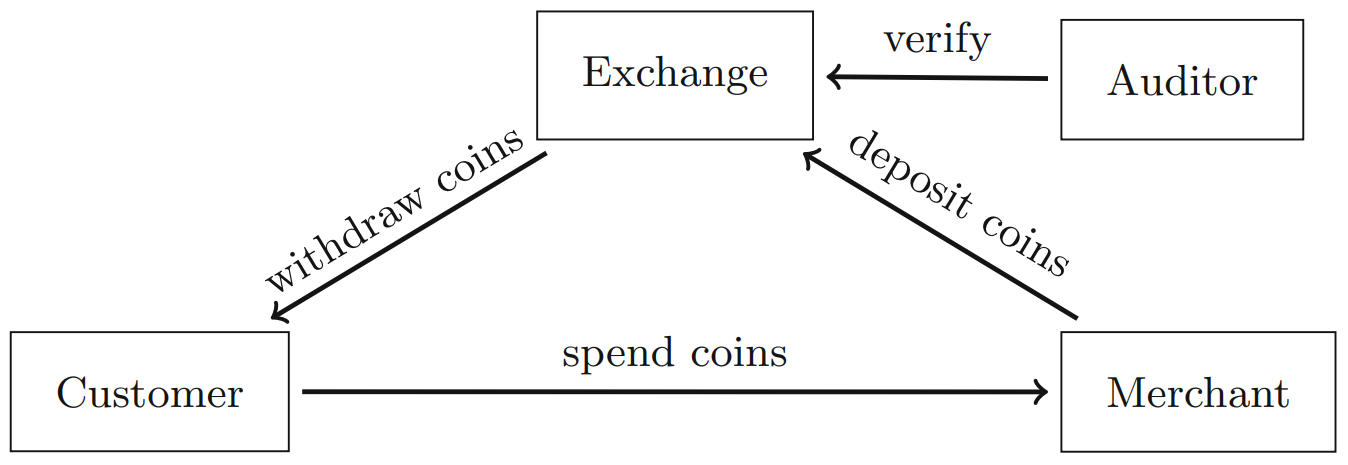
\includegraphics[width=0.7\textwidth]{gnu_system_graphic.png}
    \caption{Grundlegender Ablauf des GNU Taler Systems \cite{gnu-burdges2016enabling}}
    \label{fig:gnu_taler_overview}
\end{figure}

\textbf{Taler abheben.} Damit ein Customer Geld auf sein Wallet laden kann, muss er sich zuerst bei seiner Bank anmelden. Sollte die Bank GNU Taler native unterstützen, so kann der Customer in einem Formular eine Summe auswählen, die er in Taler übertragen möchte und einen Exchangeservice, über welchen der Tausch abgewickelt wird. Nachdem der Customer die Transaktion bestätigt hat, wird die ausgewählte Summe transferiert, der Exchangeservice signiert die äquivalente Summe an Talern und überträgt diese in das Wallet des Customers.\\

\textbf{Taler ausgeben.} Gehen wir von der Situation aus, dass ein Customer bei einem Merchant (hier ein Onlineshop) etwas erwerben möchte. Nach der Auswahl des Produktes und GNU Taler als Zahlungsmittel erstellt der Merchant einen Zahlungsvertrag, der Details wie den Gesamtpreis, mögliche offene Umwandlungsgebühren und akzeptierte Exchangeservices beinhaltet und sendet diesen an das Wallet des Customers.  Wenn der Customer daraufhin die Zahlung übermittelt, so leitet der Merchant die erhaltenen Taler direkt an den Exchange weiter. Wenn der Exchange den Eingang bestätigt, so kann der Merchant dem Customer die Transaktion bestätigen und der Kauf ist somit abgeschlossen.\\


In dem Treuhändermodell eignet sich GNU Taler aber nur teilweise als Zahlungssystem. Der Datengebende stellt dabei den Merchant dar, der seine Daten als digitales Gut anbietet. Der Datennutzende stellt hier die Rolle des Customers dar und möchte diese Daten erwerben. Sollte der Datengebende der Anfrage des Datennutzende zustimmen, so würde er einen Zahlungsvertrag formulieren, um den Anspruch auf seine Vergütung zu formalisieren. Allerdings soll der Datengebende im Datentreuhändermodell so gut wie möglich vor Informationsgewinnung geschützt werden. Bei dem von GNU Taler vorgeschlagenen Prozess wird jedoch die Identität des Datengebenden nachverfolgbar, während der Datennutzenden anonym bleibt. Zusätzlich besteht eine direkte Kommunikation zwischen Datengebenden und Datennutzenden, was weitere schützenswert Information über die Identität des Datengebenden (beispielsweise seine IP-Adresse) preisgibt.

\section{Bitcoin}
\label{sec:bitcoin}
Die Idee hinter Bitcoin entstand 2008 durch eine Person oder Gruppe mit dem Namen Satoshi Nakamoto. Heute ist Bitcoin die mit Abstand weit verbreiteteste Onlinewährung weltweit \cite{btc-beginnerGuide}. Sie basiert auf einem verteilten öffentlichen Register, das alle Transaktionen pseudonymisiert für jeden einsehbar macht und speichert. Dieses Register ist auch als Blockchain bekannt.

\begin{figure}
    \centering
    \label{fig:btc_blockchain}
    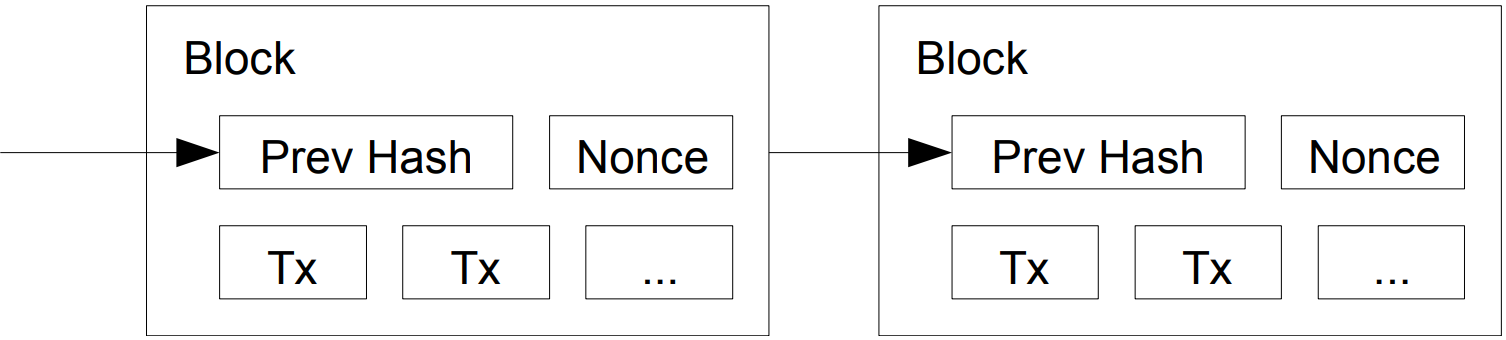
\includegraphics[width=0.5\linewidth]{BitcoinBlockchain.png}
    \caption{Blockchain mit Transaktionen \cite{btc-nakamoto2008bitcoin}}
\end{figure}

Die Blockchain ist eine Kette an Blöcken, die jeweils den Hash des vorherigen Blocks und neue Transaktionen speichert. Durch den Hash des vorherigen Blocks entsteht eine Kette, in der jeder Block Informationen über seinen Vorgänger speichert, wie in Abbildung \ref{fig:btc_blockchain} zu sehen ist. Ein neuer Block entsteht durch einen sogenannten Proof of Work. Dieser ist das Wissen über eine Zufallszahl, deren Hash mit $x$ 0 bits beginnt, welche ausschließlich durch das wiederholte Ausprobieren von Zufallszahlen gefunden werden kann. Dieser Vorgang wird als Bitcoin Mining bezeichnet. Sobald eine solche Zahl gefunden wird, kann der aktuelle Block abgeschlossen werden und alle folgenden Transaktionen werden in dem nächsten Block gespeichert \cite{btc-nakamoto2008bitcoin}.

Der Algorithmus, der bestimmt wie schwer das Erbringen des Proof of Works ist, kann jederzeit dynamisch an die Rechenleistung der Miner angepasst werden, so dass im Schnitt alle 10 Minuten ein neuer Block gefunden wird \cite{btc-Zaghloul2019Bitcoin}. Um also eine vergangene Transaktion auf der Blockchain zu verändern, müsste ein Angreifer für jeden darauffolgenden Block selbst einen Proof of Work berechnen. Ein Angreifer kann deswegen nur eine vergangene Transaktion ändern, wenn er allein mehr Rechenleistung besitzt als alle anderen Miner zusammen. \\

In dem Moment, in dem ein Block abgeschlossen und der nächste begonnen wird, sind alle Transaktionen auf dem abgeschlossenen Block ein Mal bestätigt. Das bedeutet, dass keine der Transaktionen einen Coin zum zweiten Mal ausgibt. Dies ist eine essenzielle Sicherheitsmaßnahme von Blockchain Kryptowährungen da Blockchain dezentralisiert und ohne neutralen Überprüfer funktioniert. Es ist also an allen Beteiligten, die pseudonymisierten Transaktionen des Blocks zu überprüfen. Sollte ein Angreifer die Zufallszahl finden und vor Abschluss des Blocks noch eine doppelte Ausgabe hinzufügen, so kann diese Transaktion erst festgestellt werden, wenn bereits neue Transaktionen in dem nächsten Block hinzugefügt werden. Das zeigt, dass nur weil eine Transaktion bestätigt ist, sie nicht direkt vertrauenswürdig ist. Im Fall von Bitcoin wird empfohlen, 6 weitere Blöcke abzuwarten bis eine Transaktion wirklich abgeschlossen ist \cite{btc-Zaghloul2019Bitcoin}. In Kombination mit einer durschnittlichen Berechnungsdauert von 10 Minuten dauert es also ca. eine Stunde, bis eine Transaktion auf der Blockchain als Sicher angesehen wird.
Durch den enormen Rechenaufwand, der benötigt wird um einen Block abzuschließen, kann grob überschlagen werden, wie viel Energie in eine einzelne Bitcointransaktion fließt. In \cite{btc-energyConsumption} wird eine Transaktion auf 703,25 kWh geschätzt, was ca 470.000 VISA Transaktionen entspricht.\\

Allein die lange Bestätigungsdauer einer Bitcointransaktion schließt es bereits für die Verwendung in diesem System aus, da eine Stunde nicht mehr als vernachlässigbare Zeit angesehen werden kann und somit nicht Zeitsensitiv ist. Hinzu kommt der gigantische Stromverbrauch, welcher die Skalierbarkeit von Bitcoin selbst in Frage stellt. 


\section{Ethereum}
\label{sec:ethereum}
Ethereum ist die Blockchainanwendung hinter der zweit meist verbreitetesten Kryptowährungen Ether \cite{eth-marketCapitalisation}. Es wurde 2013 von Vitalik Buterin erfunden und ist eine Plattform, die es Entwicklern ermöglicht Anwendung auf der Blockchain zu entwickeln. Es liefert eine Turing-vollständige Programmiersprache die es Entwicklern erlaub, eigene Währungen in unter 20 Zeilen Code zu schreiben \cite{eth-buterin2013ethereum}. Sämtliche dort geschriebene Währungen oder sogenannte Smart Contracts werden über die Ethereum Blockchain pseudonymisiert öffentlich zur Verfügung gestellt. 

Durch die Verwendung der Blockchain decken sich einige Eigenschaften mit Bitcoin. Es besteht genauso aus einer Reihe an Blöcken, die kontinuierlich ihren Vorgänger referenzieren. Bis 2022 nutzte Ethereum ebenfalls einen Proof of Work Ansatz. Doch seit 2022 basiert Ethereum auf einem sogenannten Proof of Stake Konzept \cite{eth-explainerInvestopia}. Das bedeutet, dass es eine Gruppe an Validierern gibt, welche die Transaktionen innerhalb der Blöcke überprüfen. Um ein Validierer zu werden, muss ein Starteinsatz von 32 Ether gezahlt werden. Alternativ kann sich ein Nutzer einem Validiererpool anschließen und einen kleineren Starteinsatz zahlen. Dafür muss er jedoch die erzielten Gewinne teilen. 

Die Aufgabe eines Validierers ist es, unzulässige Transaktionen festzustellen. Im Fall eines Angriffs auf einen Block wird der Block von Gasper (Einer Mischung des Casper-FFG Protokolls und LMD Ghost Algorithmus \cite{eth-buterin2020combining}.) markiert. Anschließend entscheiden die Validierer, ob der Block zugelassen oder blockiert werden soll. Validierer, die sich bösartig Verhalten, werden dadurch bestraft, dass ihr Starteinsatz nach und nach ``verbrannt`` wird. Mit verbrannt ist gemeint, dass der Einsatz an ein Wallet ohne Private-Key gesendet wird, was die Coins unwiderruflich unzugänglich macht. Durch diesen alternativen Ansatz kann der große Rechenaufwand von Bitcoin umgangen werden.\\

Die Verwendung einer Blockchain stellt hier wieder das Problem der Zeitsensitivität. Zwar dauert das Erstellen eines Blocks bei Ethereum nur 12 Sekunden \cite{eth-timePerBlock}. Dafür wird allerdings eine Mindestanzahl von 30 Blöcken empfohlen, bevor eine Transaktion für gültig erklärt wird. Somit entsteht eine Wartezeit von ca sechs Minuten, was bei weitem besser ist als Bitcoin. Trotzdem sind sechs Minuten keine vernachlässigbare Zeit, weshalb auch Ethereum nicht für dieses System verwendet werden kann.


\section{Privacy Pass}
\label{sec:privacy-pass}
Privacy Pass ist eine Browsererweiterung, die den Komfort der Internetbenutzung für Nutzer eines VPN erhöht. Ein VPN bietet einige Vorteile in der regulären Kommunikation über das Internet. Beispielsweise erhöht die Nutzung die Anonymität des Nutzers, da dessen private IP-Adresse so nur dem VPN-Anbieter bekannt ist und nicht dem Webseitenbetreiber. Allerdings gibt es auch Nachteile die häufig übersehen werden \cite{pp-Abbas2023Security}. Einer dieser Nachteile ist entsteht durch das Teilen einer IP-Adresse mit vielen weiteren Nutzern. So genügen wenige bösaritge Nutzer die den VPN verwenden um ihre Spuren zu verwischen, damit die IP-Adresse von einem Content Delivery Network einen schlechten Ruf erhält. Ein Content Delivery Network (kurz CDN) ist dafür zuständig, häufig angefragte Webseiten wie Google.de oder Netflix.com in seinem Cache aufzubewahren und so die Zugriffszeit, welche durch physikalisch große Distanzen zwischen Nutzer und Server, entsteht zu verkürzen \cite{pp-cdn}. Zusätzlich liefert ein CDN eine Menge an Sicherheitsfunktionen, wie unter anderem IP-Adressen mit schlechtem Ruf ein CAPTCHA präsentieren, um Botzugriffe zu verhindern \cite{pp-Ghaznavi2021Content}. Daraus resultiert, dass ein regulärer Nutzer eines VPNs erheblich mehr CAPTCHAs lösen muss als ein Nutzer, der keinen VPN verwendet \cite{pp-davidson2018privacy}.

\subsection{Umgehen vom CAPTCHAs}
Die Erweiterung ermöglicht es vorab ein CAPTCHA zu lösen und damit eine Menge an Token zu erhalten. Solange ein Nutzer über mindestens einen Token verfügt kann er das nächste Mal, wenn ein CDN ihn aufgrund eines schlechten IP-Rufwertes zum Lösen eines CAPTCHAs auffordert, stattdessen einen Token einlösen und kann die Aufgabe so überspringen. Dadurch erhöht sich die Nutzerfreundlichkeit unter der Verwendung eines VPNs, da die Anzahl an zu lösenden CAPTCHAs rapide sinkt. \cite{pp-davidson2018privacy}

\subsection{Funktionsweise}
Das System ist in eine sogenannte Signierphase und Einlösephase aufgeteilt. Die Signierphase startet, nachdem der Nutzer erfolgreich ein CAPTCHA gelöst hat. Sie ist dafür zuständig, dem Nutzer eine Anzahl an Token auszustellen, die durch den Server signiert sind. Die Einlösephase beginnt, wenn ein CDN ein CAPTCHA für den Zugang zu einem Webinhalt fordert. Bei ihr wird einer der gespeicherten signierten Token eingetauscht, um die Lösung des CAPTCHAs zu überspringen. 

\paragraph{Signierphase.} Erstellen und signieren von Token
\begin{figure}[H]
    \centering
    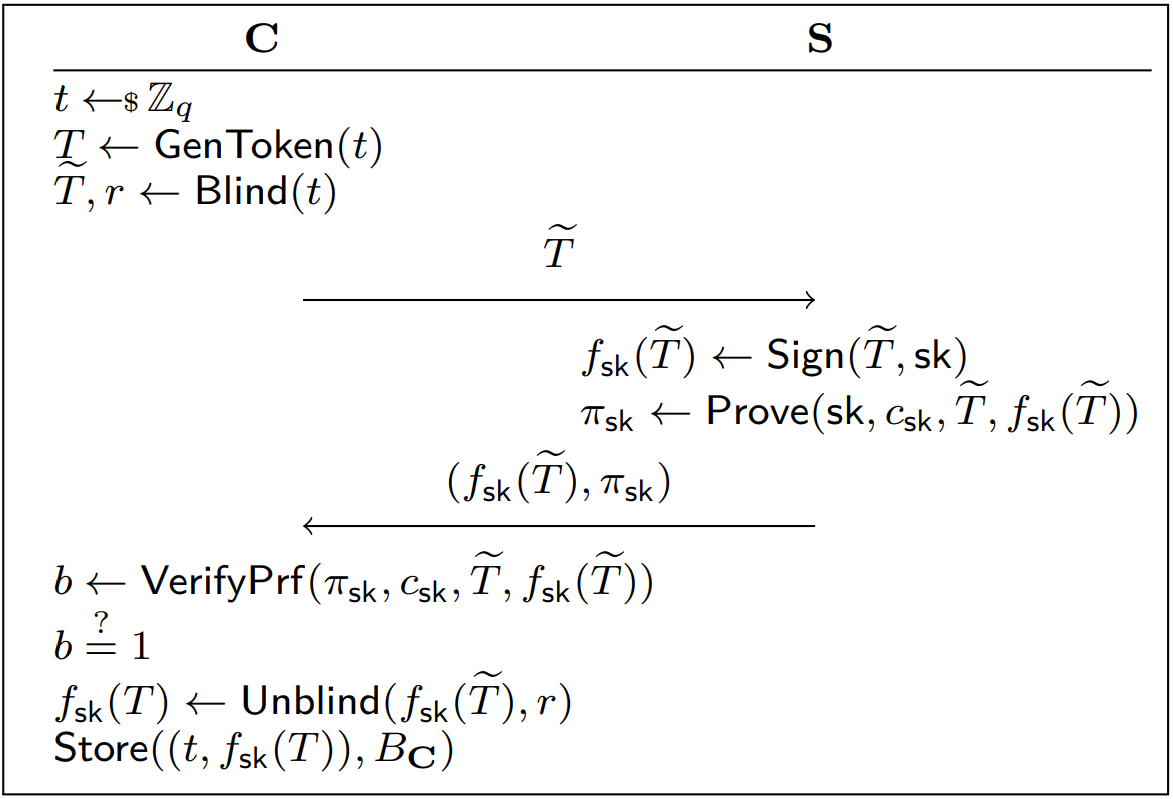
\includegraphics[width=0.5\linewidth]{pp_signphase.png}
    \caption{Signierphase von Privacy Pass \cite{pp-davidson2018privacy}}
    \label{fig:pp-signingphase}
\end{figure}
Die Abbildung \ref{fig:pp-signingphase} zeigt die Berechnung beim Durchlaufen einer Signierphase. Zuerst erstellt der Nutzer \textit{C} (Client) einen zufälligen Tokenseed $t$ mit $t {\in}_R \mathbb{Z}_q $. Daraus generiert er Token $T$ beispielsweise mit einer Hashfunktion und blendet diesen mit $r$ wie in Abbildung \ref{sec:blindSig} beschrieben, um $\widetilde{T}$ zu erhalten. Dieser geblendete Token wird nun an den Server \textit{S} gesendet, damit dieser in signieren kann. Beim Server angekommen beginnt dieser damit, den Token mit seinem privaten Schlüsselt $sk$ zu signieren. Anschließend erstellt er einen sogenannten Batch Discrete Log Equivalence Proof (BDLEQ), um dem Nutzer zu beweisen, dass er für jeden Nutzer einen gleichen Private-Key verwendet. Sollte er für jeden Nutzer einen eigenen Private-Key benutzen, so kann er den Nutzer über längere Zeit deanonymisieren, da er die in der Signierphase erhaltenen Token mit denen der Einlösephase verlinken kann. Der signierte Token und der BDLEQ werden wieder an den Nutzer gesendet, dieser prüft die Korrektheit des Beweises, unblendet den signierten Token und speichert ihn für spätere Verwendung. 

\paragraph{Einlösephase.} Signierten Token einlösen\\
\begin{figure}[H]
    \centering
    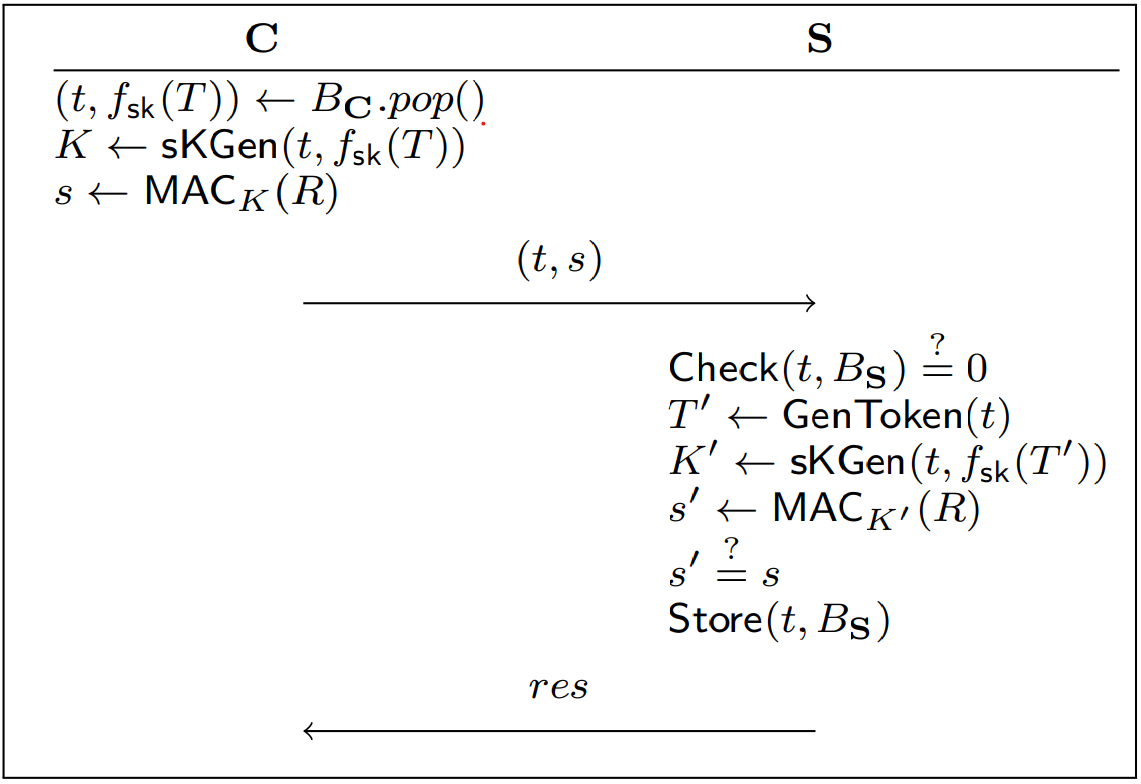
\includegraphics[width=0.5\linewidth]{pp-redemptionphase.png} 
    \caption{Einlösephase von Privacy Pass \cite{pp-davidson2018privacy}}
    \label{fig:pp-redemptoinphase}
\end{figure}
Hier zeigt Abbildung \ref{fig:pp-redemptoinphase} den Ablauf der Einlösephase, in der der Nutzer damit beginnt, einen gespeicherten signierten Token auszulesen und einen anfragenabhängigen Wert $R$ zu berechnen. Dieser könnte einfach die Domain der Anfrage sein. Er generiert einen shared Key $K$ aus dem Tokenseed und dem signierten Token und verschlüsselt $R$ mit $K$ als Key. Daraufhin sendet er das Tupel aus Tokenseed $t$ und $s\leftarrow MAC_{K}(R)$ mit shared Key verschlüsseltem $R$ an den Server. Der Server prüft, ob $t$ bereits für eine vorherige Anfrage verwendet wurde. Falls dies nicht der Fall ist, berechnet er auf Grundlage von $t$ alle Schritte des Nutzers und erhält so ein $s'$. Sollte $s'=s$ gelten, dann ist der Token valide, das CAPTCHA kann übersprungen werden und der Nutzer erhält Zugriff auf die angefragt Webressource.

\paragraph{Batch Discrete Log Equivalence Proof.}
Beim dem BDLEQ handelt es sich um einen Zero Knowledge Proof. Zero Knowledge Proofs sind ein in der Kryptographie auftretendes Beweismuster, dass das Wissen über einen Wert belegen kann ohne den Wert tatsächlich zu nennen. Der hierverwendete Discrete Log Equivalence Proof kann wie sich aus dem Namen ableiten lässt dazu verwendet werden, die Gleichheit von zwei diskreten Logarithmen zu zeigen. Für die genau Anwendung wird hier auf die Arbeit von Davidson et al. \cite{pp-davidson2018privacy} verwiesen. Dieser Beweis wird aus dem Grund erstellt, dass ein CDN ansonsten für das Signieren von jedem Token ein unterschiedliches Schlüsselpaar verwenden kann. Die Folgenden davon sind, eine mögliche Deanonynmisierung, da der CDN beim Einlösen des Tokens anhand des verwenden Signierschlüssels der einmalig ist, den Signierzeitpunkt und zugehörigen Nutzer bestimmen kann. Der DLEQ liefert dem Nutzer hier die Sicherheit, dass der diskrete Logarithmus des zum signieren verwendeten Private-Keys der gleiche ist, wie ein von CDN öffentlich bekannt gegebener diskreter Logarithmus. Davidson et al. beschreibt zudem einen Weg den DLEQ in einer Sammelform zu formulieren, sodass ein Beweis für eine Liste an Token gilt \cite{pp-davidson2018privacy}, was Rechenaufwand spart.\\\\

Im Grunde lässt sich Privacy Pass gut auf die Verwendung im Datentreuhändermodell anwenden. Unter den Annahmen, dass ein Datennutzender hier ein Nutzer ist, kann er Token bei dem Datentreuhänder erwerben, speichern und zu einem späteren Zeitpunkt wieder ausgeben. Da die Token blind signiert werden, wird vermieden, dass der Datentreuhänder die in den unterschiedlichen Phasen verwendeten Token zueinander verlinken kann und Zusammenhänge zwischen Einlösen und Ausgeben ziehen kann. Der Datentreuhänder kann eine weitere überprüfende Instanz verwenden wie in \cite{pp-davidson2018privacy} beschrieben wird, um den Aufwand der Überprüfung auszulagern. \\
Einige Punkte sprechen jedoch gegen die direkte Verwendung von Privacy Pass. 
\begin{enumerate}
    \item Die Token haben keinen Wert. Bei Bezahlungsmittel ist es essenziell einen bestimmten Preis bezahlen zu können. Dafür wären entweder mehrere unterschiedliche Tokens von Nöten oder Token, die einen monetären Wert gespeichert haben. Bei der Speicherung eines monetären Wertes erbringt sich das Problem der Beweisbarkeit. Wenn ein Token geblendet ist und für den Datentreuhänder nicht lesbar ist, wie kann sichergestellt werden, dass der richtige Wert eingehalten wurde und der Datennutzende sich nicht mehr Geld aufschreibt als ihm zusteht. Ansonsten kann nur ein Vielfaches von einem Token gezahlt werden was dazu führt, dass es keine präzise Preisvergabe gibt oder bei jeder Transaktion eine große Menge an Token validiert werden müssen.
    \item Ein Nutzer interagiert sowohl zum Einlösen als auch zum Ausgeben nur mit dem Server und nicht mit einem Verkäufer, dem er seine Token im Tausch anbietet. Es existiert hier also kein 3. Akteur wie bei GNU Taler \ref{subsec:gnu} der erhaltene Token einlöst.
    \item Die Token können ähnlich wie bei GNU Taler \ref{subsec:gnu} nicht direkt an den Verkäufer weitergegeben werden, da dadurch eine direkte Verbindung zwischen Datennutzenden und Datengebenden entsteht, welche schützenswerte Informationen offen legt.
\end{enumerate}

\section{Privacy-Preserving Reputation Management}
\label{subsec:rep}
In ihrem Paper beschreiben R Petrlic et al. ein Reputationssystem um Nutzern den Dienst eines Dienstleisters anonym bewerten zu lassen und so anderen Nutzern eine Einschätzung über die Qualität der Dienstleistung zu geben \cite{petrlic2014privacy}. Es werden 3 Rollen charakterisiert. Ein Reputation Provider $RP$, der sich um das Verwalten der verschiedenen Reputationswerte kümmert. Eine Menge an Service Providern $SP$, die einen Dienst anbieten der durch Nutzer bewertet werden soll. Und zuletzt eine Menge an Nutzern $U$, die die Dienstleistung der Service Provider bewerten. Wobei keiner der Nutzer gleichzeitig ein Service Provider $SP$ sein kann, $U \cap SP = \varnothing$. 

Der im Paper beschriebene Ablauf des Bewertens eines $sp \in SP$ durch einen Nutzer $u \in U$, umfasst grob die Erstellung eines Schemas für einen Bewertungsvektors durch $sp$, welcher von $u$ später verwendet wird, um den $sp$ zu bewerten. Nach dem $sp$ dieser Vektor mit dem $RP$ kommuniziert wurde, kann $u$ eine Dienstleistung von $sp$ in Anspruch nehmen. Dieser antwortet, zusätzlich zur Erbringung der Dienstleistung, mit einer Beschreibung des Bewertungsvektors, einem Schlüsselpaar und einem Token. Dank der Beschreibung kann der Nutzer selbst einen Bewertungsvektor erstellen, in welchen er seine Bewertung der Dienstleistung einbaut. Im Anschluss wird dieser mit dem Schlüsselpaar verschlüsselt, signiert und zusammen mit dem signierten Token an den $RP$ gesendet. Der Token dient hier zur Erkennung von doppelten Bewertungen. 

Die Berechnung der Reputation ist in Zeitslots eingeteilt, damit ein $sp$ nicht in der Lage ist einen alten Reputationswert anzugeben. Wenn nun ein Nutzer $u$ den Reputationswert eines $sp$'s einsehen möchte und der Wert für den gewünschten Zeitraum noch nicht bestimmt wurde, so muss dieser zwischen $RP$ und $sp$ berechnet werden. Hierfür bestimmt $RP$ die Summe aller verschlüsselten Bewertungsvektoren für den Zeitraum und sendet diese zusammen mit weiteren Prüfwerten an $sp$. Dieser kann die übermittelten Werte prüfen und auf eine Blacklist hinzufügen, um Replay Attacken von $RP$ auszuschließen. Wenn die Überprüfung gelingt, signiert $sp$ die Summe der Vektoren zusammen mit einer ID und verifiziert somit den neuen Reputationswert an $RP$. 

Bei einer Anfrage des Reputationswertes von $sp$ durch $u$, schickt der $sp$ eine Reihe an Werte zu $u$. Diese erlauben es $u$, den Bewertungsvektor zu interpretieren und zu prüfen, dass der übermittelte Werte sowohl aktuell, als auch nicht beeinflusst wurde. 
Das Konzept von Petrlic et al. bietet unter anderem Schutz vor: 
\begin{enumerate}
    \item \textbf{Whitewashing}, bei dem sich ein $sp$ mit schlechter Reputation als neuer $sp$ ausgeben kann, um somit den Wert zurücksetzen kann.
    \item \textbf{Transaction-independent Ratings}, bei denen ein Nutzer die Dienstleistung bewerten kann, obwohl er besagte Dienstleistung nicht in Anspruch genommen hat.
    \item \textbf{Sybil Attacks}. Ein Nutzer bewertet eine Dienstleistung unter mehreren Identitäten und täuscht so seine Meinung als Gruppenmeinung vor.
    \item \textbf{Delta Analysis}. Eine teilweise Deanonymisierung des Nutzers durch Vergleichen von gesammelten Bewertungen in unterschiedlichen Zeitabständen.
\end{enumerate} 
In der vorliegenden Situation kann das Konzept zu großen Teilen verwendet werden. Die Rollenverteilung bleibt unter den Zuweisungen von Service Provider zu Datengebenden, Reputation Provider zu Datentreuhänder und User zu Datennutzenden bestehen. Allerdings ist das Konzept darauf ausgelegt, dass zu Beginn eine Kommunikation zwischen dem Datengebenden und Datennutzenden besteht, so dass der Reputationswert direkt durch den Datennutzenden abgefragt werden kann. An dieser Stelle muss das Konzept etwas abgewandelt werden, da zu keinem Zeitpunkt während der Durchführung eine direkte Kommunikation bestehen soll. Stattdessen soll der Austausch des Reputationswertes direkt über den Treuhänder ablaufen.

\section{Blinde Signaturen}
\label{sec:blindSig}
Das von David Chaum im Jahre 1983 veröffentlichtes Paper ``Blind signatures for untraceable payments`` beschreibt den theoretischen Ansatz, dass ein Nutzer eine verifizierbare Signatur für eine Nachricht erhält, ohne dass der Unterzeichner den Inhalt der Nachricht kennt. \cite{chaum1983blind}. Ein Beispiel hierfür wäre ein Zahlungsdienstleister, der eine neuen Coin in dem Umlauf bringen möchte. Dafür sendet er seinen Reputationswert und den unkenntlich gemachten Coin an eine zentrale Institution. Wenn diese den Reputationswert als hoch genug ansieht und somit den Zahlungsdienstleister als vertrauenswürdig erkennt, so kann sie den Coin blind signieren und an den Dienstleister zurückschicken. Wenn nun ein späterer Inhaber des Coins prüfen möchte, ob sein Coin von einem vertrauenswürdigen Dienstleister erstellt wurde, so kann er die blinde Signatur mit dem Public-Key der Institution entschlüsseln. Das Ergebnis dieser Berechnung zeigt, dass die Institution den Coin tatsächlich signiert hat und sie dem Coinaussteller vertraut. Der hierbei essenzielle Punkt ist, dass diese Institution nicht weiß, was sie unterschreibt. Somit kann die Institution die Beziehung des Dienstleisters und des Coininhabers nicht nachverfolgen. 

Die für das Verfahren nötigen Rechenschritte sind im Folgenden beschrieben. Angenommen der Unterzeichnende verfügt über eine private Signierfunktion $s'$ und eine öffentliche Funktion $s$, sodass $s(s'(x)) = x$. Der Nutzer verfügt über die privaten Funktionen $c$ und dessen invers $c'$, sodass $c'(s'(c(x))) = s'(x)$. 
\begin{enumerate}
    \item Der Nutzer beginnt nun damit, sich ein $x$ auszusuchen. Dieses wird durch zufällige Redundanz vor Kollisionen geschützt und mit $c(x)$ unkenntlich gemacht.
    \item Anschließend erhält der Unterzeichnende $c(x)$, berechnet $s'(c(x))$ und schickt den entsprechenden Wert an den Nutzer zurück.
    \item Wenn der Nutzer nun $c'(s'(c(x))) = s'(x)$ berechnet, so erhält er den signierten Ursprungswert $x$ ohne, dass der Unterzeichnende $x$ je kannte.
\end{enumerate}
Daraufhin kann jede weitere Person die Unterschrift überprüfen, indem diese die öffentliche Funktion $s$ verwenden um $s(s'(x))$ zu berechnen und das Ergebnis mit $x$ abgleichen. 

Blinde Signaturen sind bei dem Ansatz von privatsphäreschützenden Zahlungs- und Reputationssystemen einer der Kernbausteine der verwendet wird, um einen vertrauenswürdigen Austausch zwischen den Parteien zu ermöglichen. Sie liefern die Grundlage der Kommunikation.

\section{Partiell Blinde Signaturen}
\label{sec:partBlindSig}
\begin{figure}[h]
    \label{fig:partBlindSig}
    \centering
    \includegraphics*[width=1\textwidth]{partBlindSig.png}
    \caption{Ablauf einer partiell blinden Signatur \cite{abe2000provably}}
\end{figure}
Partiell blinde Signaturen ähneln sich vom Effekt stark zu blinden Signaturen von Chaum aus \ref{sec:blindSig}. Der jedoch entscheidende Unterschied ist, dass es bei partiell blinden Signaturen einen Infowert gibt, der sowohl dem Nutzer als auch dem Signierendem bekannt ist. Dieser kann genutzt werden, damit der Signierende möglicherweise Prüfungen durchführen kann und zu entscheiden, ob er die Nachricht wirklich signieren möchte. Diese Eigenschaft wird im späteren Verlauf beispielsweise dazu verwendet einen Coin partiell blind zu signieren. Hierbei ist es essenziell, dass der Signierende den monetären Wert des Coins prüfen kann, da ein Nutzer sonst freie Kontrolle über den Wert seines eigenen Coins hat. Mit partiell blinden Signaturen kann genau dies gewährleistet werden. Dabei ist der monetäre Wert des Coins die Info und der kryptographische Wert des Coins die Nachricht. Nun kann der Signierende prüfen, ob der monetäre Wert der vereinbarte Wert ist und kann den kryptographischen Wert des Coins blind signieren. Der springende Punkt ist der Zusammenhang zwischen Info und Nachricht, da sonst der monetäre Wert des Coins nach dem Signieren durch den Nutzer verändert werden könnte. Um dies zu verhindern, verwendet das Verfahren den Hash der Info als Teil der Signatur, so dass diese nur gültig ist, solange die Info unverändert bleibt.

\subsection{Funktionweise}
Die Durchführung einer partiell blinden Signatur besteht aus 4 Schritten. Diese 4 Schritte sind notwendig, um die Abhängigkeit von dem msg und Info herzustellen. Es wird davon ausgegangen, dass vor dem ersten Schritt beide Parteien über den Infowert verfügen. Der Signierende bildet zuerst den Hashwert der Info, signiert diesen und schickt ihn an den Nutzer. Dieser bildet den gleichen Hashwert der Info und verwendet die erhaltenen Werte zusammen mit einer Reihe an Zufallszahlen, um $\alpha$ und $\beta$ zu berechnen. $\epsilon$ ist der darauffolgende Hash von $\alpha,\beta,z$ und $msg$. Hier fließt die bereits signierte Info über $\alpha$ und $\beta$ mit ein. Kurz darauf empfängt der Signierende $e$, welches nun sowohl Info als auch msg beinhaltet. Dieses $e$ kann er nun verwenden, um Info und msg zu signieren und die aus den Berechnungen resultierende Werte an den Nutzer zu senden. Der Nutzer kann dadurch $\rho,\omega,\sigma,\delta$ bestimmen und speichern. Möchte der Nutzer zu einem beliebigen Zeitpunkt die Signatur auf ihre Gültigkeit prüfen, so kann er $\omega + \delta$ mit  $H (g^\rho y^\omega || g^\sigma z^\delta || z || msg)$ vergleichen. Wenn die Werte übereinstimmen, ist die Signatur valide.

Durch die Verwendung von Info als Teil der Signatur ist gewährleistet, dass die Signatur nur bei einer unveränderten Info und msg valide bleibt. Denn sollte sich die Info oder msg ändern, dann würde die Rechnung zur Überprüfung einen anderen Hash erzeugen, welcher nicht mehr mit $\omega+\delta$ übereinstimmt. Insgesamt ist das partiell blinde Signaturen Schema etwas umständlicher als Chaums blinde Signaturen. Dennoch bietet es die Möglichkeit einen öffentlichen Wert zu kommunizieren und dessen nachträgliche Änderung zu verhindern.


\section{Elliptische Kurven Kryptographie}
\label{sec:ecc}
Die Kryptographie über elliptische Kurven (ECC - elliptic curve cryptography) ist ein Zweig der Kryptographie, der bereits seit 1985 besteht \cite{ecc-miller1985use} und trotz dessen nur wenig Aufmerksamkeit genießt. Hierbei geht es um das Ver- und Entschlüsseln von Nachrichten anhand von Punkten auf einem elliptischen Graph, was verglichen mit RSA, das auf der Faktorisierung großer Zahlen basiert, erhebliche Performanzsteigerung liefert.

\subsection{Trapdoor functions}
Das asymmetrische RSA Verschlüsselungsverfahren ist heute weltbekannt und wird in über 90\% der Onlinekommunikation verwendet \cite{ecc-rsa_amount}. Dessen Sicherheit basiert genauso wie die von ECC auf sog.  \textit{Trapdoor functions}. Ein Trapdoor function ist ein mathematisches Problem, welches in eine Richtung leicht zu berechnen ist, das Inverse jedoch erheblich schwerer zu bestimmen ist. Im Falle von RSA ist die Trapdoor function das Faktorisierungsproblem. Es ist leicht 2 sehr große Zahlen miteinander zu multiplizieren. Allerdings ist es deutlich schwerer bei einem gegebenen Produkt dessen Faktoren zu bestimmen, insbesondere wenn die Faktoren jeweils Primzahlen sind. Dies ist der Grund, weshalb RSA sicher ist und zuverlässig die Kommunikation schützt. Bei ECC ist die Trapdoor function, die die Sicherheit der Verschlüsselung ausmacht, eine andere. Jedoch kann anhand dieser genauso ein Public und Private-Key generiert werden.
\subsection{Funktionsweise}
Um die Trapdoor function hinter ECC zu verstehen, müssen wir uns zuerst elliptische Kurven anschauen. Die algebraische Struktur von elliptische Kurven ist eine Gruppe, welche aus einer Menge von Punkten $M$ und einer binären Operationen $\circ$ auf 2 Punkten der Menge besteht. Die Definition einer Gruppe fordert, dass die Elemente die Eigenschaften der Assoziativität, Identität, Existenz eines inversen Elements und je nach Quelle auch Abgeschlossenheit erfüllen. \cite{ecc-aradi2016einfuhrung}\cite{ecc-bogopolskij2008introduction} Zudem müssen die Koordinaten aller Punkte $(x,y) \in M$ die in der Menge liegen, aus dem endlichen Feld stammen, sowie die Gleichung:

\begin{equation}
    \label{ecc-equation}
    y^2 = x^3+ax+b
\end{equation} erfüllen. Zusammen bildet die Menge an Punkten $M$ einen Graph, der je nach Wahl der Parameter $a,b$ einer Form aus Abbildung \ref{fig:ecc_1} ähnelt. Aufgrund der Gleichung \ref{ecc-equation} entsteht der Zusammenhang, dass eine Gerade durch zwei zufällig gewählte Punkte $P,Q \in M$, den Graph immer an genau einer dritten Stelle schneidet. Zusätzlich ist der Graph an der X-Achse durch das $y^2$ gespiegelt. Mit diesen Eigenschaften kann nun die Operation $\circ$ definiert werden.\\
Diese arbeitet wie folgt: Bei Eingabe von $A,B \in M$ finde den invertierten dritten Schnittpunkt mit dem Graph. Dieser sei hier mit $C$ beschrieben. Eine Ausführung von $A \circ B = C$ ist in Abbildung \ref{fig:ecc_2} verdeutlicht.

\begin{figure}
    \centering
    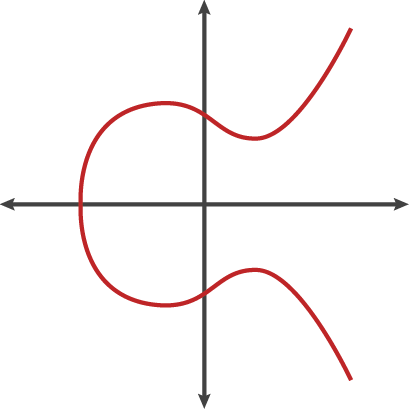
\includegraphics[width=0.4\textwidth]{ecc_1.png}
    \caption{Mögliche Form einer elliptischen Kurve \cite{ecc-cloud2013elliptic}}
    \label{fig:ecc_1}
\end{figure}
\begin{figure}
    \centering
    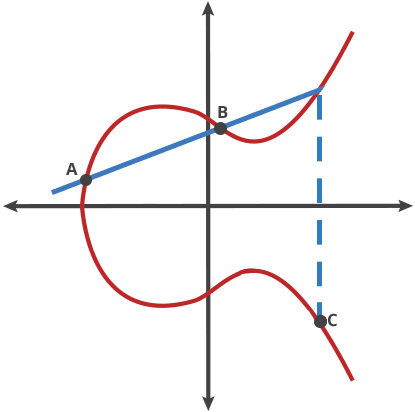
\includegraphics[width=0.4\textwidth]{ecc_2.png}
    \caption{Operation $\circ$ auf Punkten $A,B \in M$ \cite{ecc-cloud2013elliptic}}
    \label{fig:ecc_2}
\end{figure}
\begin{figure}
    \centering
    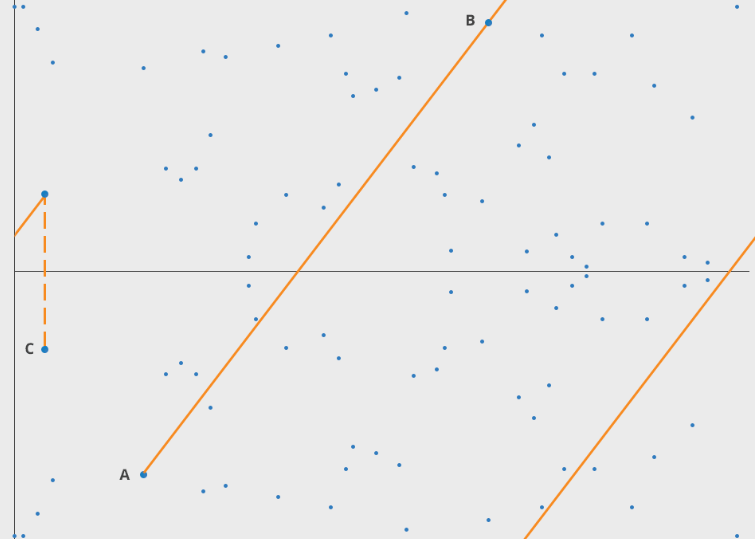
\includegraphics[width=0.4\textwidth]{ecc_3.png}
    \caption{Graph nach Anwendung von $\mathbb{Z}_p$ \cite{ecc-cloud2013elliptic}}
    \label{fig:ecc_3}
\end{figure}

Die Operation $\circ$ kann beliebig oft hintereinander mit dem jeweils neu entstehenden Punkt ausgeführt werden. Genau hier liegt die Trapdoor function von ECC. Mit Kenntnissen über der Startpunkt $A$ und die Anzahl der Ausführungen $n$, ist es einfach den Endpunkt $E$ zu berechnen. Wenn allerdings nur der Endpunkt $E$ und Startpunkt $A$ gegeben sind, ist es sehr rechenaufwändig die Anzahl an Ausführungen zu bestimmen.

\subsection{Anwendung in der Kryptographie}
Allgemein ist zu beachten, dass elliptische Kurven, die für ein kryptographischen Verwendung in Frage kommen, eine andere Form haben als die eben aufgeführt Abbildungen (\ref{fig:ecc_1},\ref{fig:ecc_2}). Entscheidend ist hierfür die Wahl des endlichen Feldes. In der Kryptographie wird hier meist $\mathbb{Z}_p$ verwendet. Diese Wahl bringt 2 Eigenschaften mit sich:
\begin{enumerate}
    \item Das $p$ in $\mathbb{Z}_p$ besagt, dass alle Werte $x \in \mathbb{Z}_p$, $0 \leq x \leq p-1$ erfüllen müssen. Durch die Wahl dieses Wertebereichs, können die X und Y-Achse nie den Wert $p$ überschreiten, sondern beginnt anstatt wieder bei 0.
    \item Die zweite Eigenschaft ist die ausschließliche Betrachtung ganzer Zahlen als X und Y-Koordinate. Hierdurch wird aus dem Graphen eine Menge an zufällig aussehend gewählten Punkten. Der Graph für die kryptographische Verwendung einer elliptischen Kurve ist ein Abbildung \ref{fig:ecc_3} visualisiert.
\end{enumerate}
Nun muss ein passendes $p$ sowie $a,b$ bestimmt werden, um die genaue Menge an Punkten zu spezifizieren. Hierfür gibt es bereits eine große Auswahl und Werten in der Literatur \cite{ecc-lochter2010elliptic}\cite{ecc-merkle2013elliptic}. Eine der prominentesten ist die ``Curve25519`` von Daniel J.Bernstein \cite{ecc-bernstein2006curve25519}. Sie hat den Werte $p=2^{255}-19$ (daher der Name) und die elliptische Funktion $y^2=x^3+486662x^2+x$.


\subsection{Vor- und Nachteile}
Allgemein betrachtet ist die Tatsache, dass ECC eine schnellere Berechnungszeit liefert als RSA nicht von der Hand zu weisen \cite{ecc-cloud2013elliptic}. Da sich die Laufzeiten von Verschlüsselung und Entschlüsselung durch RSA und ECC asymptotisch nicht gleich verhalten, ist es schwer eine endgültige Antwort zu nennen. Allerdings schlägt ECC RSA bei der Gesamtzeit für Ver- und Entschlüsselung je nach Nachrichtengröße um einen Faktor von \textasciitilde $3-20$ \cite{ecc-mahto2018performance}\cite{ecc-bao2022research}. Zudem eignet sich ECC vor allem als Ver- und Entschlüsselungsmethode auf rechenschwachen Geräten wie Mobiltelefonen aufgrund von kleineren Schlüsselgrößen\footnote{Um eine Security Bit Level von 256 Bits mit RSA zu erreichen, ist eine Schlüssellänge von 15360 Bits nötig, während es bei ECC lediglich 512bits sind.\cite{ecc-mahto2018performance}}. So können Rechenaufwand, Energieverbrauch und RAM-Auslastung gesenkt werden \cite{ecc-gupta2011ecc}.

Allerdings wurde 2007 bekannt, dass der Pseudo Random Number Generator (PRNG) Dual\_EC\_DRBG eine potenzielle Backdoor hat, die es Nutzern mit Informationen über einen bestimmen Wert die Zufälligkeit problemlos knacken lies \cite{ecc-green2013backdoor}. Dual\_EC\_DRBG wurde 2005-2006 zusammen von NIST (National Institute of Standarts and Technology) und der NSA veröffentlicht und basiert die Auswahl der zurück gegebenen pseudozufälligen Zahlen auf Berechnung über elliptischen Kurven. Dieser Vorfall schwächt bis heute das generelle Vertrauen in ECC. \cite{ecc-cloud2013elliptic}

\section{AES - Advanced Encryption Standard}
\label{sec:aes}
Der Advanced Encryption Standard ist einer der weltweit am häufigsten verwendeten symmetrischen Verschlüsselungsalgorithmen. AES wurde 2001 vom NIST als offizieller Standard für die Verschlüsselung von Daten festgelegt und hat den früher verwendeten Data Encryption Standard (DES) ersetzt, da dieser als unsicher galt. AES basiert auf dem Rijndael-Algorithmus, der von den Kryptographen Joan Daemen und Vincent Rijmen entwickelt wurde. Die hohe Sicherheit, Effizienz und Flexibilität von AES haben dazu beigetragen, dass er heute in einer Vielzahl von Anwendungen, von vertraulichen Regierungsdokumenten bis hin zur Verschlüsselung von Festplatten und Netzwerkverkehr, zum Einsatz kommt.

AES ist ein blockbasierter Verschlüsselungsalgorithmus, der Daten in Blöcken von 128 Bit verarbeitet. Dabei verwendet AES symmetrische Schlüssel, was bedeutet, dass derselbe Schlüssel sowohl für die Verschlüsselung als auch für die Entschlüsselung der Daten verwendet wird. Der Algorithmus unterstützt Schlüsselgrößen von 128, 192 und 256 Bit, wobei größere Schlüssel im Allgemeinen eine höhere Sicherheit bieten, jedoch auch höhere Rechenressourcen erfordern. AES durchläuft mehrere Runden von Transformationen, die die Klartextdaten in scheinbar zufällige Chiffretextdaten umwandeln. Bei der 128-Bit-Schlüsselgröße umfasst der Algorithmus 10 Runden, bei 192-Bit sind es 12 Runden und bei 256-Bit werden 14 Runden verwendet. Jede dieser Runden besteht aus mehreren Schritten, darunter Substitution (Byte Substitution mittels S-Box), Zeilenverschiebung (ShiftRows), Spaltenmischung (MixColumns) und die Hinzufügung eines Rundenschlüssels (AddRoundKey).

Das zentrale Sicherheitsmerkmal von AES ist seine Widerstandsfähigkeit gegen bekannte Kryptoangriffe wie Differenzial- und Linearkryptanalyse. Dies wird durch eine starke Schlüsselabhängigkeit und die Nutzung mehrerer kryptographischer Prinzipien, wie der Substitutions-Permutations-Netzwerkstruktur (SPN), erreicht. Darüber hinaus spielt die sogenannte Avalanche-Eigenschaft eine entscheidende Rolle: Eine kleine Änderung im Klartext oder im Schlüssel führt zu drastischen Änderungen im Chiffretext, wodurch es Angreifern erschwert wird, Rückschlüsse auf den ursprünglichen Klartext oder den verwendeten Schlüssel zu ziehen.\\

Verglichen mit asymmetrischen Verschlüsselungsverfahren fehlen AES jedoch gewisse Schutzziele die über die letzten Jahre zunehmend an Wichtigkeit gewonnen haben. Die Verwendung von einem einzelnen Schlüssel führt dazu, dass es die Integrität einer Nachricht nicht gezeigt werden kann, was bedeutet, dass Veränderungen an der Nachricht, die nicht vom ursprünglichen Sender stammen nicht festgestellt werden können. Aus diesem Grund haben Sadi Arman, Shamim Al Mamun und Nuray Jannat einen modified AES Algorithmus (MAES) veröffentlicht, der durch die Verwendung weitere Bit Verschiebeoperationen eine Senderauthentifizierung, Empfängerauthentifizierung und Nachrichtenintegrität gewährleisten kann \cite{aes-arman2024modified}. Der Algorithmus beschränkt die für AES üblichen Schlüssellängenauswahl von 128, 192 und 256-bit Schlüsseln auf ausschließlich 128-bit Schlüssel, erhöht dafür aber gleichzeitig die Datenübertragungsrate um bis zu 20\% \cite{aes-arman2024modified}.

\section{Abschluss}
%pro und contra von allen
Aus dieser Liste an verwandten Arbeiten geht hervor, dass es noch kein Bezahlsystem gibt, das den in \ref{chap:req} aufgestellten Anforderungen gerecht wird. Die Tabelle \ref{tab:nichtfunktionale_Anforderungen} gibt dabei einen Überblick über die vorgeschlagenen Lösungsansätze und welche der Anforderungen durch sie nicht erreicht werden.
\begin{table}[H]
    \centering
    \begin{tabular}{|c|c|c|c|c|}
        \hline
        & GNU Taler & Bitcoin & Ethereum & Privacy Pass \\
        \hline
        Anonymität & $\times$  & \texttildelow & \texttildelow & $\checkmark$ \\
        \hline
        Unverkettbarkeit & $\times$  & \texttildelow & \texttildelow & $\checkmark$ \\
        \hline
        Zeitsensitivität & $\checkmark$ & $\times$ & $\times$ & $\checkmark$ \\
        \hline
        Skalierbarkeit & $\checkmark$ & \texttildelow & $\checkmark$  & $\checkmark$\\
        \hline
        Vertraulichkeit & $\checkmark$ & $\checkmark$ & $\checkmark$ & \texttildelow \\
        \hline
        Integrität & $\checkmark$ & $\checkmark$ & $\checkmark$ & \texttildelow \\
        \hline
    \end{tabular}
    \caption{Erfüllung nichtfunktionaler Anforderungen}
    \label{tab:nichtfunktionale_Anforderungen}
\end{table}
GNU Taler erfüllt jede der Anforderungen -- abgesehen von der Anonymität. Zwar schützt GNU Taler die Anonymität des Käufers und hält dessen Privatsphäre aufrecht, allerdings sollte ein im Datentreuhändermodell verwendetes Bezahlsystem hauptsächlich die Privatsphäre des Verkäufers schützen, die von GNU Taler gezielt öffentlich gemacht wird.

Bitcoin und Ethereum teilen sich aufgrund der Verwendung einer Blockchain das Problem von nicht zeitsensitiven Transaktionsdauern. Mit einer geschätzten Wartezeit von einer Stunde bzw. 6 Minuten, bis eine Transaktion mit ausreichend Sicherheit bestätigt werden kann, ist die Verwendung der beiden Technologien unter Einhaltung der Anforderungen nicht möglich. Des Weiteren kann argumentiert werden, dass durch den Public Ledger, der alle Transaktionen pseudonymisiert veröffentlicht, die Anonymität nur in Teilen gewahrt werden kann. 

Vertraulichkeit und Integrität werden durch Privacy Pass nicht nativ unterstützt. Da das Protokoll ausschließlich für das Umgehen von CAPTCHAs bei CDNs entwickelt wurde, ist von einer https-Verbindung auszugehen, die diese Schutzziele gewährleistet. Jedoch sieht Privacy Pass selbst keine Maßnahmen zum Schutz der Kommunikation vor.\\

Aufgrund dessen, dass keines der zuvor genannten Bezahlsysteme sämtliche Anforderungen erfüllt, muss für den Anwendungsfall im Datentreuhändermodell ein neues Bezahlsystem entworfen werden. Dieses Bezahlsystem wird in dem folgenden Kapitel genauer beschrieben und spezifiziert. 


%==================================================================================================



\chapter{Systementwurf}
\label{chap:systems}
%reputation, grober ablauf, auf welchem rl basiert, präziser ablauf in der Schrittbeschreibung

In diesem Kapitel werden die neu erarbeiteten Systeme genau beschrieben. Dafür werden zu Beginn einige Designentscheidungen und Ziele des Systems genannt. Anschließend wird für jedes der drei Systeme ein detailierter Ablauf beschrieben und weitere wichtige Informationen für die Funktionsweise der Systeme genannt.

\section{Ziel}
\label{sec:mainPart_ziel}
Um einen privatsphäreschützenden Anreiz für die Benutzung eines Datentreuhänders zu schaffen wird im Folgenden ein Bezahlsystem vorgestellt. Dieses Bezahlsystem erlaubt es den Datengebenden für ihre Daten im Gegenzug einen finanziellen Ausgleich zu verlangen, ohne dabei persönliche Informationen preisgeben zu müssen. Weder der Datennutzende noch der Datentreuhänder kann bei einer regulären Transaktion bestimmen, welcher Datengebende eine Bezahlung erhält. Der hierfür verwendete Ablauf sieht vor, dass ein Datengebender zuerst seine Daten an den Datennutzenden überträgt und ihm etwas Zeit zur Verwertung der Daten lässt. Ein Datennutzender erhält maximal 12 Stunden Zeit, um den Zahlvorgang abzuschließen. Schafft er dies nicht innerhalb der 12 Stunden, so kann der Datentreuhänder ihn von der weiteren Verwendung der Plattform ausschließen. 

Damit der Datengebende seine Anonymität nicht ausnutzen kann, gibt es 2 Mechanismen zur Betrugserkennung. Der erste ist eine Offenlegung der Kommunikation im Streitfall. Sollte sich eine der beiden Parteien betrogen fühlen, so kann sie vom Datentreuhänder eine Schlichtung verlangen. Dafür werden die für die Kommunikation verwendeten Einmalschlüssel dem Datentreuhänder mitgeteilt, sodass dieser alle Schritte nachvollziehen kann und entscheiden kann, ob ein Betrug vorliegt oder nicht. 
Der zweite Mechanismus ist eine Reputationsvergabe. Wenn ein Datengebender besonders qualitativ gute Daten liefert, kann ein Datennutzender ein gute Bewertung für ihn ausstellen, was seine Reputation verbessert. Wenn er hingegen besonders schlechte Daten liefert, so kann ein Datennutzender sich weigern ihn zu bezahlen, was die Reputation herunterzieht. Des Weiteren kann bei jedem Aufruf nach Daten von einem Datennutzenden ein Reputationsschwellwert festgelegt werden, um Datengebende mit zu schlechter Reputation von dem Einreichen ihrer Daten abzuhalten. 

\section{Geld als Anreiz}
Da im Datentreuhandmodell ein Datennutzender meist durch ein Unternehmen oder eine Forschungseinrichtung repräsentiert wird, ist es vorstellbar, dass der Datennutzende selbst eine Dienstleistung anbieten oder in Aussicht stellen kann. Hier wurde aber Geld als Anreiz gewählt, da die Verwendung solcher Dienstleistungen als Anreiz einige Nachteile mit sich ziehen kann.

\begin{enumerate}
    \item \textbf{Universal.} Kein Handelsgut oder Dienstleistung ist so universelles begehrt wie Geld. Zwar ist es möglich, dass ein Business, welches hier als Datennutzender auftritt, für die Preisgabe der Daten eine Dienstleistung anbietet. beispielsweise können Social Media Plattformen wie X kostenlose zeitlich bedingte Premiumabonnenments oder vergleichbar Angebote in Aussicht stellen. Jedoch ist das Interesse an solchen Angeboten subjektiv, was sie als mögliche Anreize zwar denkbar aber eher suboptimal macht.
    \item \textbf{Einheitlich.} Wenn der Anreiz durch den Datennutzenden gestellt wird, wird dieser in jedem einzelnen Fall unterschiedlich sein. Aus der Kommunikationsstruktur folgt, dass alle unterschiedlichen Kompensationen auf irgendeinem Weg über den Datentreuhänder laufen müssen. Daraus ergibt sich ein enormer zusätzlicher Aufwand an Entwicklung und Implementation für jeden Datennutzenden.
    \item \textbf{Verfügbarkeit.} Manche Datennutzende, wie beispielsweise Forschungsinstitutionen, haben nur eine eingeschränkte Auswahl an Dienstleistungen oder Produkte die sie Datengebenden anbieten können. Da sie hauptsächlich an der Forschung interessiert sind, verfügen sie über erheblich weniger Konsum- oder Unterhaltungsprodukte verglichen mit anderen Firmen. Geld ist hingegen deutlich leichter zugänglich.
    \item \textbf{Wahrung der Anonymität.} Viele C2B Treuhänder legen Wert auf die Anonymität oder Pseudonymität der Datengeber. Diese kann jedoch dadurch, dass ein Datennutzender die versprochene Dienstleistung kontrolliert, verloren gehen. Es ist beispielsweise denkbar, dass ein Datennutzender einen vielversprechenden Anreiz verspricht, diesen aber hinter einer Registrierung und Angaben von persönlichen Daten verbirgt, so dass die durch den Treuhänder etablierte Anonymität umgangen wird.
    \item \textbf{Einhalt der Leistung.} Der Datentreuhänder kann bei der Auslagerung von Anreizen an den Datennutzenden nicht zuverlässig kontrollieren, dass der Datennutzende die versprochene Dienstleistung wirklich einhält.
\end{enumerate}
Durch die Verwendung von Geld als Anreiz werden diese Punkte umgangen. Das Interesse der Datengebenden ist nun ausschließlich abhängig von dem Ruf und dem persönlichen Interesse an einem Datengebenden und nicht von dessen Anreizangebot. Der Anspruch auf den versprochenen Anreiz ist für jeden Datennutzenden gleich implementiert und hängt maximal von der Wahl anderer Parameter ab. Es kann davon ausgegangen werden, dass alle Datennutzenden über Geld verfügen und dieses als Kompensation verwenden können. Aufgrund des Stellenwertes von Geld in unserer Gesellschaft sind bereits viele Wegen entwickelt worden, wie dessen Wert anonym oder pseudonym an andere übertragen werden kann. Der Datentreuhänder hat die volle Kontrolle darüber, dass ein zu zahlender Geldbetrag vom Datennutzenden abgegeben wird und auch bei Datengebenden ankommt.

\section{Annahmen über das Datentreuhändermodell}
\label{sec:systemAssumptions}
Datentreuhänder können in verschiedenen Variation eingesetzt werden. Abschnitt \ref{sec:dt} gibt darüber bereits einen Überblick. Hier werden Annahmen getroffen, die das Datentreuhändmodell betrefen, für welches das Anreizsystem entworfen wird. Dadurch soll verdeutlicht werden, in welchem Datentreuhändermodell das System am besten eingesetzt werden kann.

Zuerst sei anzunehmen, dass es sich bei dem Datentreuhänder um einen freiwilligen Customer to Business Treuhänder handelt. Dies ist dadurch begründet, dass bei verpflichtenden Datentreuhändern die Benutzung vorgeschrieben ist und ein Anreiz zur Benutzung des System die Nutzerzahlen nicht beeinflusst. Weiter haben bei Business to Business Treuhändern beide Parteien einen Profit aus dem Tausch der Daten. Beide sind gleichzeitig am Daten empfangen und am Daten versenden. Hier fällt daher eine deutliche Einteilung in Datengebende, die Anreize erhalten und Datennutzende, die Anreize bieten, schwer. Zusätzlich ist die Aussicht auf Datengewinn durch einen Tausch häufig Anreiz genug, um ein Unternehmen zur Verwendung eines B2B Datentreuhänders zu bewegen. \todo{proof}

Die beim Datentreuhänder abgelegten Daten sind verschlüsselt. Der Datentreuhänder speichert lediglich eine lange Liste an Bytes, kann aber anhand der verschlüsselten Bytes nicht feststellen, was die Daten beinhalten, welche Daten von welchem Datengebenden stammen oder wo ein Datensatz aufhört und der nächste beginnt. Er weiß also nichts über die bei ihm abgelegten Daten. Damit ein Datengebender trotzdem den Zugang zu seinen Daten behält, werden ihm beim Hochladen seiner Daten, Werte für den kontreten Ablageort seiner Daten, sowie einen passenden Schlüssel zur Entschlüsselung mitgeteilt. Wenn er seine abgelegten Daten nun einsehen möchte, kann er den Satz an Bytes von dem Speicherort anfragen und den erhaltenen Geheimtext mit Hilfe des Schlüssels entschlüsseln, was seine ursprünglich hochgeladenen Daten zum Vorschein bringt.

Es gibt 2 Paradigmen bezüglich der Auswahl von Datengebenden. Das erste davon umfasst den Sachverhalt, dass ein Datengebender dem Datentreuhänder erklärt, dass er seine Daten zum Verkauf anbieten möchte. Der Datentreuhänder bewirbt darauf die Daten des Datengebenden auf einer -- einem Marktplatz vergleichbaren Plattform -- und Datennutzende wählen sich die Datengebende ihre Wahl aus und beziehen von ihnen die angeboten Daten. Das zweite Paradigma dreht die Zuständigkeit um. Hier kann ein Datennutzender einen Aufruf starten, der Datengebende dazu aufruft, Daten eines bestimmen Typen zu verkaufen. Jetzt können sich Datengebende durch eine Liste an Aufrufen durcharbeiten und den Richtig für sich heraussuchen. Sobald ein passender Aufruf entdeckt wurde, kann ein Datensatz des vom Datennutzenden angefragen Datentyps vorgelegt werden. 
Im Folgenden wird vom zweiten Paradigma ausgegangen, da es sowohl Rechenaufwand- als auch Privatsphärenvorteile liefert. Das Erstellen eines Aufrufs sowie das Weiterleiten zum Datentreuhänder sollte beides in $O(1)$ geschehen. Dadurch hängt die Laufzeit von der konkreten Implementierung ab, allerdings beinhaltet das Erstellen eines Aufrufs nur die Zusammensammlung von Informationen wie Datentypen, Namen oder Beschreibung. Es sind in meisten Fällen keine iterativen Vorgänge aktiv, die die Laufzeit in $O(n)$ bringen könnte. Im Anschluss sind keine weiteren Berechnungen von Nöten um Daten zu empfangen. Bei der individuellen Auswahl von Datengebenden und der Nachfrage nach deren Daten entsteht hingegen ein Zusammenhang zwischen der Anzahl an Datensätzen und des Rechenaufwands des Datennutzenden. Da der Datennutzende für jeden Datengebenden eine Bewertung erzeugen muss, die darüber entscheidet ob die Daten erworben werden oder nicht, ergibt sich für den Erhalt von $n$ Datensätzen ein Rechenaufwand von $O(n)$. Die Minimierung des Rechenaufwands für den Datennutzenden ist vor allem interessant, da Datennutzende durch Unternehmen repräsentiert werden, die in Extremfällen mehrere tausend Anfragen pro Sekunden bearbeiten müssen, während Datengebende an ihren Endgerät einen deutlich überschaubareren Rechenaufwand leisten müssen.
Privatsphärenvorteile werden durch das zweite Paradigma ebenfalls erbracht, da die Einreichung von Daten so vollständig anonym ablaufen kann. Solange durch die Kommunikation zur Mitteilung des Speicherorts und Datenschlüssels keine Informationen preisgegeben werden, kann der Datennutzende den Datengebenden unmöglich deanonymisieren. Die von ihm erhaltenen Datenparameter können dazu benutzt werden, Daten beim Datentreuhänder zu erfragen. Dieser weiß genauso wenig, wessen Daten angefragt wurden. Im ersten Paradigma hingegen müssen mindestens die Informationen, die ein Datennutzender braucht um eine aussagekräftige Einschätzung über die Daten trefen zu können, bereitgestellt werden. Je nach dem welche Informationen davon betroffen sind, besteht eine Möglichkeit, die Angebote eines Datengebenden miteinander zu verlinken und so Informationen über ihn zu gewinnen.

 

\section{Generelles}
%PKI für schlüssel assumen
Im Gegensatz zu GNU Taler soll das Bezahlsystem hauptsächlich den Datengebenden und dessen Informationen schützen. Die Privatsphäre des Datennutzenden ist zwar ebenfalls schützenswert aber eher von geringerer Bedeutung, da im Datentreuhändermodell der Datennutzende meist durch ein Unternehmen oder eine Forschungseinrichtung dargestellt wird. Hinzu kommt die Struktur eines Datentreuhänders, die den Datennutzenden dazu veranlasst, eine Menge an Informationen anzugeben, um vom Datentreuhänder zugelassen zu werden. Der Datengebende hingegen ist eine einzelne Privatperson, die ihre gesammelten Daten bewusst an Unternehmen oder Forschungseinrichtungen verkaufen möchte. Der Schutz der Privatperson ist hier daher von größerem Interesse. 

Unter diesen Umständen ist eine herkömmliche Überweisung per Bank deutlich zu unsicher. Sie benötigt Information wie die IBAN des belasteten Kontos und die IBAN des empfangenden Kontos, um zu wissen, von wo nach wo eine Geldsumme fließen soll. Dadurch werden bereits zu viele Informationen über den Datengebenden bekannt, da der Datennutzende nun genau herausfinden kann, von wem die erworbenen Daten stammen und ob er bereits vorher schon von demselben Datengebenden Daten gekauft hat. Zusätzlich kann die Bank nachvollziehen, dass eine Privatperson sich als Datengebender angemeldet hat und wem sie ihre Daten bereits verkauft hat.
Um dieses Problem zu lösen, wird hier eine der gängigsten anonymen Onlinezahlmethoden verwendet: Kryptowährungen. Die Abschnitte \ref{subsec:gnu}, \ref{sec:bitcoin}, \ref{sec:ethereum}, \ref{sec:privacy-pass} führen bereits einige davon auf und beschreiben, warum diese nicht im Datentreuhändermodell verwendbar sind. Aufgrund dessen wird hier eine neues System eingeführt. Jedoch ist dessen Coins weder Blockchain basiert noch für Spekulationszwecke brauchbar. Ein Coin kann -- so wie bei vielen Kryptowährungen üblich -- ausschließlich bei einem Exchange gegen Geld getauscht werden. Bei dem initialen Tauschen mehrerer Coins ist der monetäre Wert in Euro fest im Coin gespeichert und kann nicht verändert werden. 

An dieser Stelle ist anzumerken, dass keine Regulierungen oder Identifizierung zum Erwerben eines Coins benötigt werden. Jedoch sind Datennutzende die einzigen, die Coins sicher ausgeben können. Das wird dadurch deutlich, dass das Bezahlsystem nur dazu verwendet werden kann, Coins von Datennutzenden zu Datengebenden zu übertragen. Datengebende können zwar selbst auch Coins erwerben, allerdings ist der Handel nicht über das hier eingeführte Bezahlsystem möglich. Daher bleibt nur der reguläre Tausch, welcher außerhalb des Systems stattfindet und keine Betrugserkennung besitzt. Unter der Berücksichtigung dessen, dass das Einzige was dem Coin einen festen Wert sicherstellt die Signatur des Exchanges ist, kann leicht ein nicht verifizierter Coin erstellt werden und im unsicheren Tausch angeboten werden. Der andere Tauschpartner hat keine Möglichkeit den Coin vor Abwicklung des Tauschs auf seine Echtheit zu prüfen, was ein großes Potentiall für Betrug bietet. Aufgrund dessen ist anzunehmen, dass nur Datennutzende Coins erwerben werden, da der Tausch unter Datengebenden deutlich zu unsicher ist.

Nachdem ein Datennutzender einen Coin erworben hat, kann er diesen lokal so lange speichern, bis er ihn ausgeben möchte. Sobald ihm ein Datengebender seine Daten mitteilt, hat der Datennutzende 12 Stunden Zeit die Daten auszuwerten. Wenn ein Datennutzender nach Ablauf der 12 Stunden noch keine Transaktion zu dem Datengebenden abgeschlossen hat und dieser bei dem Datentreuhänder eine Betrugsanklage gegen den Datennutzenden vorlegt, so kann der Datentreuhänder sich dazu entschließen den Datennutzenden entweder zeitlich bedingt oder dauerhaft von der weiteren Verwendung der Plattform auszuschließen. Ein gutwilliger Datennutzender kann nach der Auswertung der Daten eine passende Summe an Coins aus seinem lokalen Speicher auslesen und an den Datengebenden senden. Sobald dieser die Coins empfängt prüft er die Signatur der Coins. Wenn die Signatur mit der des Exchanges übereinstimmt, kann er sie an den Exchange weiterleiten um sich den monetären Wert beispielsweise auf sein Konto gut schreiben zu lassen. Stimmt die Signatur nicht mit der des Exchanges überein, so kann der Datengebende auch hier wieder einen Betrug beim Datentreuhänder melden.

\section{Verschlüsselung}
Da in der Kommunikation indirekt Geld transferiert wird, ist es von höchster Priorität, die gesendeten Nachrichten vor dem Mithören oder Verändern durch unbefugte Dritte zu schützen. Für diesen Schutz wird eine Mischung aus der in Abschnitt \ref{sec:ecc} erklärten elliptischen Kurven Kryptographie und dem in Abschnitt \ref{sec:aes} angeführten MAES-Algorithmus verwendet. 

Mit der Benutzung eines Public-Keys bei ECC wird sichergestellt, dass nur Personen mit Wissen über den zugehörigen Private-Key die Nachricht lesen können. Anschließend wird ein Hash der verschlüsselten Nachricht gebildet und mit dem Private-Key des Senders signiert. Auf diesem Weg kann der Empfänger die Nachricht selbst den Hash bilden und prüfen, ob der signierte Hash mit dem selbst gebildeten übereinstimmt. Dadurch kann sowohl die Vertraulichkeit als auch die Integrität der Nachricht sichergestellt werden.

AES hingegen verwendet nur einen Schlüssel, der gleichzeitig zum Verschlüsseln und Entschlüsseln einer Nachricht gebraucht wird. Es erreicht erheblich schnellere Berechnungszeiten als ECC, da AES auf Operationen basiert, die lediglich bit verschieben, aber keine komplexen mathematischen Berechnungen durchführen. Da AES aber keine Integrität gewährleisten kann, wird hier für die symmetrische Kommunikationsverschlüsselung der MAES-Algorithmus verwendet. Durch ihn kann -- wie bei ECC -- eine unbemerkte Veränderung der Nachricht ausgeschlossen werden, während trotzdem nur ein Schlüssel zum Ver- und entschlüsseln benötigt wird.\\

Es sei angemerkt, dass von hieran folgend jede Nachrichtenübertragung zwischen 2 Akteuren -- dies mögen beispielsweise Datentreuhänder und Datengebender sein -- immer via ECC verschlüsselt und signiert wird, es sei denn es wird für den Kommunikationsschritt anders definiert.

\section{Notationserklärung}
In den Systementwürfen werden alle Kommunikationsschritte mit ihren übertragenen Informationen beschrieben. Für die konkrete Angabe der übertragenen Informationen wird die folgende Notation verwendet.
\begin{itemize}
    \item Datengebende sind mit $DG$, Datennutzende mit $DN$, Datentreuhänder mit $DT$ und Exchange mit $EX$ abgekürzt.
    \item $pk$ steht für Public-Key und $sk$ für Secret oder Private-Key.
    \item Ein Tupel wird $(...)$ gekennzeichnet. Es zeigt die Menge an Informationen die in einer Nachricht zwischen zwei Akteuren enthalten ist.
    \item Verschlüsselung wird mit ${\{Nachricht\}}_{Schl\textit{ü}ssel}$ dargestellt. Dabei sind alle in den Klammern enthaltenen Informationen die Nachricht und der untere Teile der Schlüssel. Daher ist ${\{ID\}}_{pk}$ eine Verschlüsselung der $ID$ und ${\{ID\}}_{sk}$ eine Signatur der $ID$.
    \item Listen an Informationen sind mit $[Nachricht]$ markiert. Sie zeigen dass eine Tupel eine Reihe an $Nachrichten$ speichert. Wie viele Einträge zulässig sind, hängt von der genauen Situation ab.
    \item Ein Element zufällig aus einer Menge wählen, wird mit $element {\in}_{R} Menge$ dargestellt.
\end{itemize}

\section{Coin Generierungsphase}
\label{system:coingeneration}
Hier werden die Coins, die im späteren Verlauf beider Systeme verwendet werden, vom Datennutzenden erstellt und vom Datentreuhänder signiert. Die einzelnen Schritte sind in Abbildung \ref{fig:coin-generationphase} verdeutlich und werden im Folgenden beschrieben.
\subsection{Ablauf}
\begin{figure}[H]
    \centering
    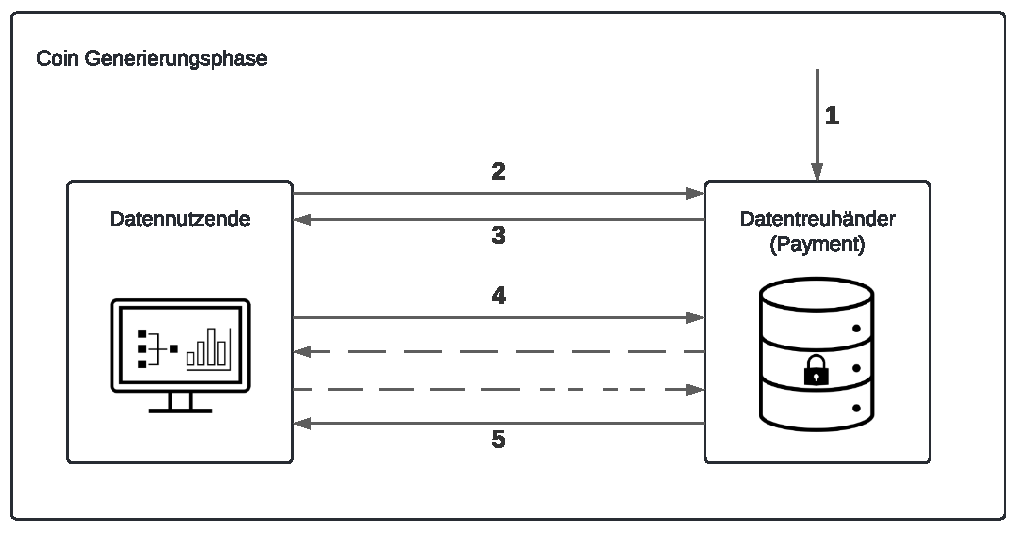
\includegraphics[width=0.9\linewidth]{CoinGenerationPhaseDiagramm.pdf}
    \caption{Coin Generierungsphase Ablauf}
    \label{fig:coin-generationphase}
\end{figure}

\paragraph{1. Zahlungseingang} $(apk \leftarrow AccountPublicKey, ES \leftarrow ErhalteneSumme)$\\
Der Exchange erhält über einen beliebigen Weg eine Summe und einen Konto Public-Key. Die genaue Umsetzung des Zahlungseingang liegt bei dem Exchange. Er kann alles zwischen einer Banküberweisung mit der $apk$ als Verwendungszweck bis hin zu einem Briefumschlag mit Bargeld und einem leserlich aufgeschriebenen $apk$ sein. Nach Eingang einer Zahlung erstellt der Exchange einen sogenannten $CoinGenerationToken$, bestehend aus $(nonce, apk, ES, spent \leftarrow false)$, verschlüsselt ihn mit dem $apk$ und speichert diesen intern. Der $CoinGenerationToken$ wird verschlüsselt, da sonst jede andere Person die den $apk$ mitgeschnitten hat selbst den Token verwenden kann, um Coins für sich zu generieren.

\paragraph{2. CoinGenerationToken abrufen} $(apk)$\\
Da der Exchange nur den $apk$ erhält hat er keine Möglichkeit den $CoinGenerationToken$ einem Datennutzenden zuzuweisen. Jetzt kann jeder beliebige Nutzer alle Einträge für einen $apk$ abfragen. Allerdings ist nur der Datennutzende in der Lage den $CoinGenerationToken$ zu entschlüsseln, der den passenden secret Key zum $apk$ hat. Dies ist im Idealfall nur der Datennutzende der die Transaktion getätigt hat.

\paragraph{3. CoinGenerationToken übertragen} $([\{(nonce, apk, ES)\}_{apk}])$\\
Auf eine $CoinGenerationToken$ Anfrage des Datennutzenden antwortet der Exchange mit allen noch nicht eingelösten Token für den $apk$. Nachdem der Datennutzende die Token erhalten hat kann er diesen zuerst mit dem passenden Private-Key entschlüsseln. Im Anschluss kann er selbst Coins erstellen. Ein Coin besteht aus $(nonce, value)$. Bei der Erstellung sind 2 Sachen zu beachten: Zuerst muss der summierte Wert aller erstellten Coins gleichgroß sein wie die $ES$ des Tokens. Des Weiteren gibt es eine Menge an möglichen Werten $MW$, sodass $\forall value\in MW$ gilt. Dies ist vor allem wichtig, da $value$ beim Signieren und Einlösen des Coins für den Exchange sichtbar ist und dieser bei einer Wahl eines selten vorkommenden $value$ eine Verbindung zwischen den Phasen herstellen kann.

\paragraph{4. Signierung Anfragen} $((nonce, apk, ES), [value])$
Eine Signieranfrage ist der Start eines Durchlaufs von partiell blinden Signaturen, bestehend aus einem $CoinGenerationToken$ und einer Menge an $values$. Zuerst kann der Exchange prüfen, ob der gesendete Token noch nicht eingelöst wurde. Anschließend summiert er alle $value$ auf und prüft, ob die Summe gleich dem $ES$ des Tokens ist. Wenn beide Überprüfungen akzeptieren, kann der Exchange mit dem partiell blind signieren anfangen und bei seinem gespeichert Token $spent \leftarrow true$ setzen um eine doppelte Einlösung zu verhindern.

\paragraph*{Gestrichelte Pfeile} $([a,b]), ([e])$\\
Die Pfeile zwischen 4. und 5. sind hier gestrichelt eingetragen, da sie notwendige Kommunikationsschritte von partiell blinden Signaturen abbilden. Sie sind essenziell für die Funktionsweise und wurden bereits in \ref{sec:partBlindSig} erklärt, weshalb sie hier nur zur Vollständigkeit aufgelistet werden.

\paragraph{5. Signieranfrage Antwort} $([r,c,s,d], \pi_{sk})$ \\
Vorausgesetzt alle Überprüfungen aus Schritt 4 akzeptieren, so erhält der Datennutzende nun eine Menge an partiell blinden signierten Coins und kann diese für spätere Verwendung lokal speichern. Zusätzlich berechnet der Exchange einen BDLEQ auf dem gleichen Weg, wie er in \ref{sec:privacy-pass} beschrieben ist. Nachdem der Datennutzende diesen verfiziert hat, kann er sicher sein, dass der Exchange zum signieren seiner Coins den selben Private-Key verwendet hat wie für die Signatur aller Coin Generierungsphasen. Sollten die Überprüfungen nicht akzeptieren so kann der Datennutzende entweder bei Schritt 4 mit anderen Coins oder bei Schritt 2 wieder ansetzen.\\

Auf diese Weise kann ein Datennutzender Geld bei einem Exchange einzahlen und eine dem Geldbetrag entsprechende Menge an Coins erhalten, ohne dass der Exchange die von ihm ausgehändigten Coins nachverfolgen kann. Gleichzeitig ist es für einen Datennutzenden nicht möglich Coins zu erhalten, für die er keinen monetären Gegenwert bereitgestellt hat.
\subsection{Finanzierung des Exchange}
Zusätzlich ist zu erwähnen, dass Exchanges finanziell motiviert sein können oder eine Gebühr verlangen möchten, um beispielsweise laufende Serverkosten zu decken. Sollte dies der Fall sein, kann vor dem Beginn der Coin Generationphase vom dem Exchange eine feste Gebühr ausgerufen werden. Wenn sich ein Datennutzender trotz der Gebühr dazu entscheidet diesen Exchange zu verwenden, so kann der Exchange nach dem Eingang einer Zahlung in Schritt 1 einen $CoinGenerationToken$ erstellen, welcher die Gebühr bereits abzieht. Wenn also ein Datennutzender eine Transaktion von $100$\texteuro\ bei Exchange mit $10\%$ Gebühr tätigt, so erstellt der Exchange einen $CoinGenerationToken$ für den angegebenen $apk$ mit $ES \leftarrow 90$\texteuro. Auf diese Weise kann eine Exchange seine finanziellen Interessen geltend machen. 

\section{Bezahlvorgang}
\label{system:payment}
Nachdem die Coins erstellt und signiert sind kann das Ausgeben dieser Coins behandelt werden. Dafür gibt es das Bezahlsystem,  welches den Datennutzenden erlaubt die Daten von Datengebenden anzufragen. Diese können der Anfrage nachkommen, wofür sie der Datennutzende im Gegenzug mit den Coins entlohnt. Damit bei dem Vorgang die Privatsphäre des Datengebenden so gut wie möglich geschützt wird, findet der Austausch der Daten und Coins über Postfächer beim Datentreuhänder statt. Dadurch entsteht keine direkte Kommunikation zwischen Datengebenden und Datennutzenden, die welche potenziell schützenswerte Informationen wie IP-Adresse oder dergleichen preisgibt. Wie der Ablauf genau funktioniert wird im Folgenden erklärt.

\subsection{Ablauf}
\begin{figure}[H]
    \centering
    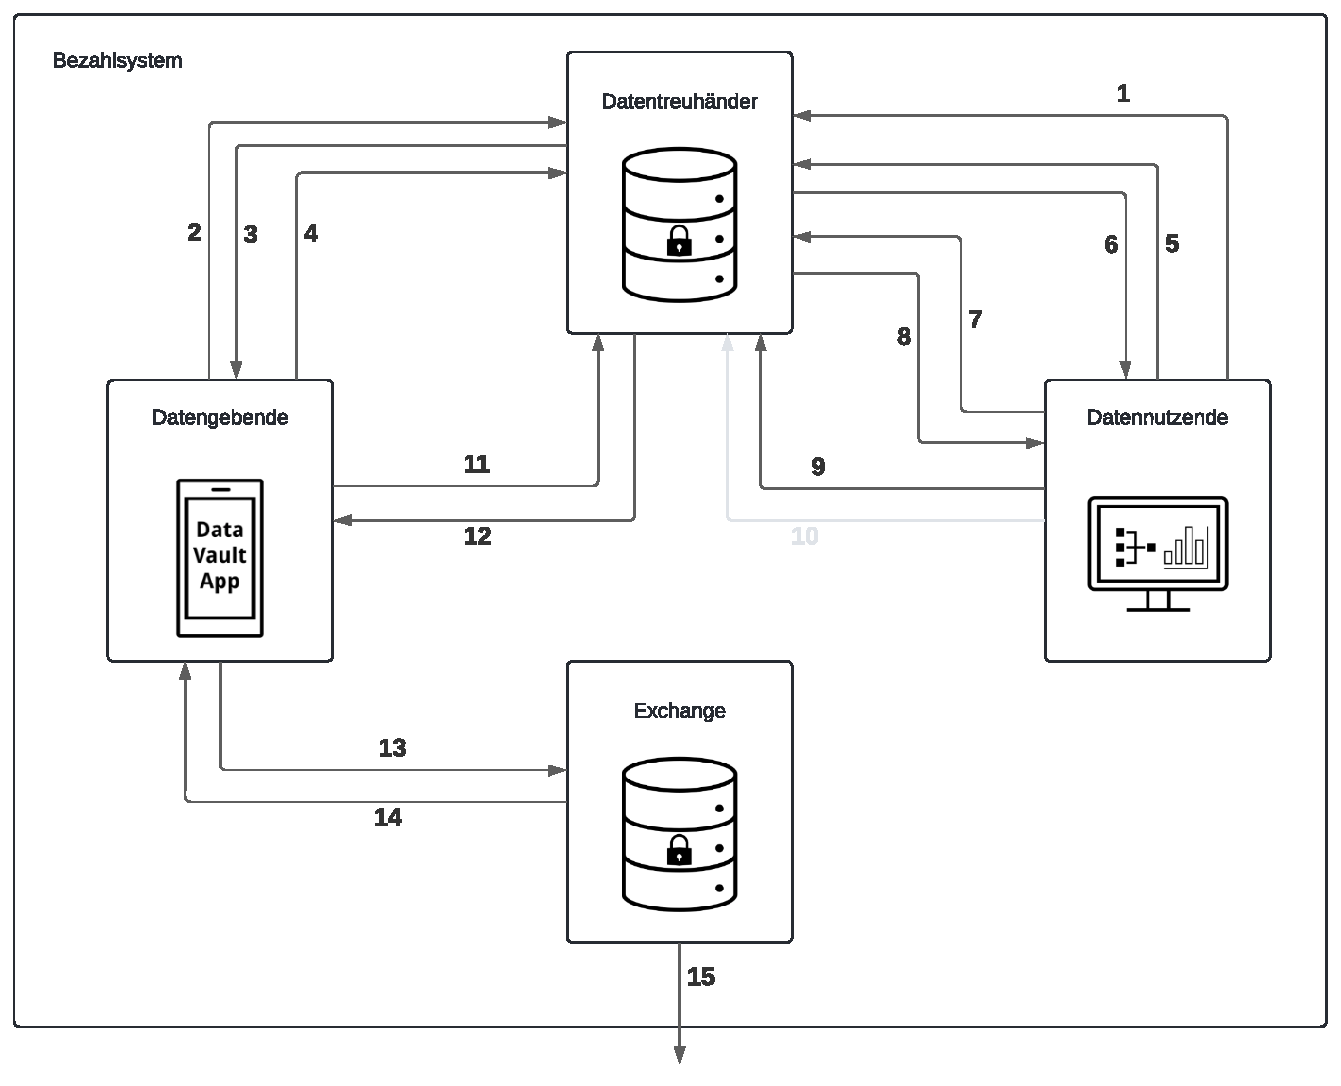
\includegraphics[width=0.9\linewidth]{PaymentDiagramm.pdf}
    \caption{Bezahlsystem Ablauf}
    \label{fig:payment}
\end{figure} 

In der Abbildung \ref{fig:payment} sind die Pfeile mit den Nummern 7,8 und 12 grau markiert. Dies hat den Grund, dass das Diagramm den gesammten Kommunikationsfluss zeigt und diese drei Schritt nur für das Bewertungssystem relevant sind, welches in Abschnitt \ref{system:reputation} beschrieben wird. Deswegen folgt die Auflistung und Erklärung der übertragenen Informationen erst in Abschnitt \ref{system:reputation}.

\paragraph{1. Aufruf starten} $(datatype, reputationThreshold, price)$\\
Der Datennutzende erstellt beim Datentreuhänder einen Aufruf zur Datenteilung. Damit verkündet er an alle Datengebenden, dass er Daten von einem bestimmten Typ sucht und benennt direkt, wieviel er für diese Daten bereits ist zu bezahlen. Da der Datennutzende nach Anlegen des Aufrufs direkt Daten erhalten kann, für die er Zahlen muss, braucht es eine Möglichkeit um ein gewisses Vertrauensminimum festzulegen. Der $reputationThreshold$ gibt dabei einen Schwellwert an, so dass der Aufruf nur für Datengebende mit einer Reputation über diesem Schwellwert sichtbar ist.


\paragraph{2. Aufrufliste anfragen} $(DG-ID, {\{DG-ID\}}_{DG-sk})$\\
\todo{nach repsystem verschieben und salt einbauen}
Damit ein Datengebender über die Liste an allen aktuell laufenden Aufrufen bescheid weiß, muss er diese Liste beim Datentreuhänder anfragen. Dafür sendet der Datengebende seine $DG-ID$, um dem Datentreuhänder seine Identität zu nennen und die $DG-ID$ welche mit seinem Private-Key signiert ist. Damit kann der Datentreuhänder den Public-Key des Datengebenden aus einer Datenbank laden, da angenommen wird, dass jeder Datengebende sich bei der Registrierung auf einen Public-Key festlegt. Mit diesem Public-Key kann der Datentreuhänder die Signatur Überprüfen und dadurch sicher sein, dass der Datengebende tatsächlich der ist, der er vorgibt zu sein. Nun kann der Datentreuhänder die Reputation des Datengebenden abrufen und für die Zusammenstellung der Aufrufliste verwenden.

\paragraph{3. Aufrufliste Antwort} $([callDetails, DN-pk])$\\
Nachdem der Datengebende seine Identität bewiesen hat, kann der Datentreuhänder seine lokale Datenbank mit Aufrufen durchsuchen und alle Aufrufe, die einen Reputationsschwellwert niedriger als die Reputation der Datengebenden haben in eine Liste aufnehmen. Damit enthält jeder Eintrag der Liste aus dem Public-Key des Datennutzenden der den Aufruf gestartet hat und Aufrufdetails, die wichtige Informationen bezüglich des Aufrufs geben. Die genauen Inhalte der Aufrufdetails sind Treuhänderabhängig, da je nach Gebiet des Treuhänders verschiede Details über den Datennutzenden für die Entscheidung des Datengebenden wichtig sein können. In den meisten Fällen umfassen die Aufrufdetails Daten wie die angefragte Datentypkategorie (GPS-Daten, persönliche Daten, etc.), den Namen des Datennutzenden, den Preis den jeder Datengebende ausgezahlt bekommen soll, einen Titel oder eine Beschreibung. Auch Informationen darüber, ob es sich bei dem Datennutzenden um eine Forschungseinrichtung handelt, können hier kommuniziert werden.


\paragraph{4. Daten teilen} $(DN$-$pk, \{Shared-Key\}_{DN-pk}, \{referenceCode, dataLocation, dataKey\}_{Shared-Key})$\\
Der Datengebende hat die genannten Aufrufdetails erhalten und sich dazu entschieden, seine Daten für einen Aufruf mit einem Datennutzenden zu teilen. Generell gilt wie in \ref{sec:dt} erklärt, dass ein Datengebender seine Daten nicht selbst speichert, sondern sie verschlüsselt beim Datentreuhänder lagert. Er behält nur den Speicherort und Schlüssel der Daten, um jederzeit Zugriff auf diese zu haben. Um seine Daten mit einem Datennutzenden zu teilen, genügt es daher den Speicherort und Schlüssel zu übertragen.

Für die Übertragung des Speicherorts und Schlüssels wird ein Postfach beim Datentreuhänder verwendet. So kann ein direkter Austausch zwischen Datengebenden und Datennutzenden verhindert werden. Ein Datengebender kann Ort und Schlüssel verschlüsselt in das Postfach legen und nur der Datennutzende, der das Wissen über den passenden privaten Schlüssel besitzt, kann Ort und Schlüssel wieder entschlüsseln.

Einer der Betrugserkennungsmechanismen ist die Offenlegung der Kommunikation im Streitfall, so dass der Datentreuhänder die Nachrichten einsehen kann und entscheiden kann, welche der Parteien recht hat. Damit bei dieser Offenlegung nur genau die Nachrichten entschlüsselt werden, die Teil einer spezifischen Kommunikation zwischen Datengebenden und Datennutzenden sind, wird für jede Abwicklung eines Tausches ein neuer symmetrischer Schlüssel erstellt.\\

Damit ein Datengebender einen Eintrag in das Postfach zu Teilen von Daten senden kann, muss er zuerst die folgenden Informationen bestimmen. Zuerst wird der Public-Key des Datennutzenden im Klartext angegeben, da ein Datennutzender beim Abfragen des Postfaches so bestimmen kann, welche Einträge für ihn bestimmt sind. Anschließend wird ein neuer symmetrischer Schlüssel Shared-Key erstellt. Dieser wird mit dem Public-Key des Datennutzenden verschlüsselt, damit dieser den Shared-Key kennt. Nun kann der Datengebende den Shared-Key verwenden um das Tupel aus $dataLocation$, $dataKey$ und $referenceCode$ zu verschlüsseln. Hierbei sind $dataLocation$ und $dataKey$ die eben beschriebenen Speicherort und Schlüssel der Daten beim Datentreuhänder. Dabei sei angemerkt, dass sowohl $dataLocation$ als auch $dataKey$ mehr als nur eine Variable sein können und von dem vom Datentreuhänder verwendeten Speicherverfahren und Verschlüsselungsverfahren abhängen. Der $referenceCode$ ist eine zufällige Zahl die später bei Schritt 9 verwendet wird, um eine Zugehörigkeit von Übertragen der Daten und Coins herzustellen.

\paragraph{5. Datenpostfach abfragen} $(DN$-$pk)$\\
Der Datennutzende kann sich zu einem beliebigen Zeitpunkt dazu entscheiden, alle Nachrichten die den angegeben Public-Key enthalten anzufragen. Dafür muss er den gewünschten Public-Key mitübertragen, um den Datentreuhänder zu signalisieren, an welchen Nachrichten er interesse hat. Der Public-Key muss hier bei jeder Anfrage spezifiziert werden, da zum einen keine Form an Authentifizierung stattfindet und jeder alle Nachrichten eines Public-Keys anfragen kann. Zum anderen bleibt dem Datennutzenden so die Möglichkeit offen, für jeden Aufruf ein eigenes Schlüsselpaar zu verwenden. Dies kann beispielsweise große Vorteile bei der internen Organisierung haben.

\paragraph{6. Datenpostfach Antwort} $([\{Shared-Key\}_{DN-pk}, \{referenceCode, dataLocation, dataKey\}_{Shared-Key}])$\\
Nachdem der Datentreuhänder die Anfrage an das Datenpostfach erhalten hat, erstellt er eine Liste mit Postfacheinträgen, die den Public-Key der Anfrage im Klartext angegeben haben. Die einzelnen übertragenen Postfacheinträge können dabei auf den Public-Key verzichten, da dieser nur zu Identifizierung genutzt wird. Der Datennutzende kennt den Public-Key ohnehin da er ihn in der Anfrage definiert. Die vollständige Liste aller Postfacheinträge kann zurück an den Datennutzenden gesendet werden.

\paragraph{9. Daten anfragen} $(dataLocation)$\\
Der Datennutzende kann nun für jeden empfangenen Postfacheintrag den passenden Private-Key verwenden, um den Shared-Key des Eintrags zu entschlüsseln. Solange der Datengebende sich an das Protokoll gehalten und den Schlüssel, den er zum Verschlüsseln des Datentupels verwendet hat auch als Klartextschlüssel angegeben hat, funktioniert dieser Schritt einwandfrei und der Datennutzende erhält Zugang zu $dataLocation$, $dataKey$ und $referenceCode$. Jetzt kann er den Datentreuhänder nach den Daten an der angegebenen $dataLocation$ fragen, welche mit dem $dataKey$ verschlüsselt sind.

\paragraph{10. Daten Antwort} $(\{data\}_{dataKey})$\\
Die durch die $dataLocation$ beschriebenen Daten werden durch den Datentreuhänder ausgelesen. Da auch hier wieder keine Authentifizierung stattfindet, kann jeder einen beliebigen Datensatz beim Datentreuhänder anfragen und erhält die an der Stelle gespeichert Daten. Da allerdings nur der Datennutzende, der den $dataKey$ vorher erhalten hat die Daten lesen kann, ist das wahllose Anfragen von Daten beim Treuhänder sinnlos, da ohne Wissen über die $dataLocation$ nur Teile eines Datensatzes oder Überlappungen in andere Datensätze geschehen können, die verschiedene $dataKeys$ benötigen würden. Der Datentreuhänder kann daher mit den ausgelesenen Daten antworten ohne Schlüsse ziehen zu können, wer die Daten angefragt hat oder ob die Nachfrage Teil eines Tausches zwischen Datengebenden und Datennutzenden ist.

Nach Erhalt der verschlüsselten Daten kann der Datennutzende den zu den Daten gehörenden $dataKey$ verwenden, um die Daten zu entschlüsseln und an den Klartext zu gelangen. Jetzt kann der Datennutzende die Daten für seine Zwecke verwerten.

\paragraph{12. Coins in Postfach legen} $(referenceCode, \{[nonce,value]\}_{Shared-Key})$\\
\label{para:payment_9}
Mit der Verwertung abgeschlossen kann der Datennutzende nun den Datengebenden bezahlen. Dafür lädt er eine Liste an Coins aus seinem Speicher, die in der Summe gleich dem im Aufruf ausgeschrieben Preis sind. Er verwendet den in Schritt 6 erhaltenen Shared-Key um die Liste an Coins zu verschlüsseln. Anschließend verwendet er den ebenfalls in Schritt 6 erhaltenen $referenceCode$, um zusammen einen Eintrag an das Coinpostfach zu senden.

Da der $referenceCode$ von dem Datengebenden mit dem Shared-Key verschlüsselt wurde, ist davon auszugehen, dass ein Eintrag mit dem gleichen $referenceCode$ nur von dem Datennutzenden stammen kann, der den Aufruf gestartet hat und die Daten erhalten und verwertet hat.

\paragraph{13. Coinpostfach abfragen} $(referenceCode)$\\
Da ein Datengebender nach dem Erstellen eines Datenpostfacheintrags den dort genutzten $referenceCode$ lokal als offen abspeichert, kann er nun bei Bedarf den Datentreuhänder fragen, ob es bereits einen Eintrag in dem Coinpostfach mit diesem $referenceCode$ gibt. Er kann somit den Datentreuhänder fragen, ob er für das Teilen seiner Daten bereits bezahlt wurde.

\paragraph{14. Coinpostfach Antwort} $(\{[nonce,value]\}_{Shared-Key})$\\
Wenn der Datennutzende bereits einen Eintrag mit den verschlüsselten Coins eingesendet hat, so werden die unter dem $referenceCode$ angegebenen verschlüsselten Coins an den Datengebenden zurückgegeben. Der Datengebende kann daraufhin den Shared-Key, welcher in Kombination mit dem $referenceCode$ gespeichert wurde verwenden, um die erhaltenen Coins wieder zu entschlüsseln. Wenn er anschließend die Liste an Coins erhält, kann er überprüfen, ob die Summe der Coins auch den Preis des Aufrufs ergibt und die partiell blinde Signatur, die in der Coin Generierungsphase Schritt 4. und 5. ausgestellt wurde, auch tatsächlich valide ist. Sollten diese Tests beide akzeptieren, so kann der Datengebende die Coins lokal speichern, bis er sie einlösen möchte.

\paragraph{15. Coins einlösen} $([nonce,value], adresse, DG-ID, \{DG-ID\}_{DT-sk})$\\
Ein Datengebender kann seine angesammelten Coins jederzeit einem Exchange senden. Dafür kann er die in Schritt 14 gespeicherten Coins aus dem Speicher lesen und gesammelt oder einzeln an einen Exchange übertragen. Um bösartigen Verhalten des Datennutzenden vorzubeugen, wird die ID des Datengebenden zusammen mit einer Signatur dieser vom Datentreuhänder, zum Einlösen der Coins benötigt. Durch die Signatur der ID wird sichergestellt, dass ein Datengebender tatsächlich seine eigene ID angibt und diese nicht beliebig durchtauschen kann. Ohne die Datengebenden ID kann ein Datennutzender eine Menge an Coins übertragen und selbst wieder einlösen bevor der Datengebende die Chance dazu erhält. Zusätzlich wird eine Form einer Zahlungsadresse -- oben $adresse$ -- zum Exchange gesendet. Bei der Implementation wird das Übertragen einer IBAN verwendet, allerdings ist es genauso gut möglich stattdessen eine Bitcoin Walletadresse oder eine beliebige andere Zahlungsmöglichkeit zu verwenden. Ein Exchange kann auch mehrere Zahlungsoptionen gleichzeitig anbieten. In dem Fall muss die Zahlungsoption als zusätzlicher Parameter mit übertragen werden.

\paragraph{16. Bestätigung} $([nonce, message])$\\
Nachdem die Coins beim Exchange eingetroffen sind überprüft dieser, ob die Coins bereits vorher schon eingelöst wurden und ob die partiell blinde Signatur gültig ist. Nachdem alle Tests durchlaufen sind, generiert er eine Liste die für jeden $nonce$ eine $message$ speichert. Für diese $message$ gibt es vier Möglichkeiten. Wenn die Tests auf Doppelausgebung und partiell blinde Signaturen akzeptieren, so wird $\{``ok''\}$ in die $message$ geschrieben. Wenn die Validierung der partiell blinden Signatur fehlschlägt, so wird $\{``blindSig validation failed'', nonce, \{``blindSig validation failed'', nonce\}_{EX-sk}\}$ in die $message$ geschrieben. Fällt beim überprüfen auf, dass der Coin bereits von einem anderen Datengebenden eingelöst wurde, so wird $\{``already spent'', nonce, \{``already spent'', nonce\}_{EX-sk}\}$ in die $message$ geschrieben. Falls der Coin von dem selben Datengebenden vorher eingelöst wurde ist die $message$ nur $\{error with spending\}$. Anschließend wird die Liste mit allen $nonce$ und deren $messages$ zurück an den Datengebenden gesendet.

\paragraph{17. Geld austeilen} $(address)$\\
Hier wird abschließend eine ausgehende Zahlung vom Exchange zu der angegebenen Zahlungsadresse in Höhe aller vollständig eingelösten Coins getätigt. Die genau kommunizierten Daten sind hier von der Zahlungsoption abhängig. Allerdings muss hier sichergestellt werden, dass der ausgehende Betrag genau dem Wert der eingelösten Coins gleicht.

\subsection{Verwendung von Proxys und TLS} \todo{TLS nutzt RSA}
Damit eine vollständige Anonymität erreicht werden kann, müssen sowohl Datengebende als Datennutzende ihre Nachrichten in den Schritten 4,7,12 und 13 über einen Proxy senden. Die Aufgabe des Proxys ist hier die Verschleierung der IP-Adresse. Durch das Weiterleiten durch einen Proxy bleibt die wahre IP-Adresse des Datengebenden bzw. Datennutzenden geheim. Ohne diesen Proxy kann der Datentreuhänder über die IP-Adresse mehrere Nachrichten miteinander verbinden und über längere Zeit mitschneiden, welcher Datengebende oder Datennutzende an wie vielen Handeln beteiligt war. Zugegebenermaßen ist eine dauerhaft gleichbleibende IP-Adresse eine Seltenheit. Der IPv4 Adressraum ist bereits seit mehreren Jahren erschöpft, weshalb IPv4 Adressen in regelmäßigen Abständen neu an aktuell sendende Geräte verteilt werden \todo{proof}. Trotzdem bleibt die IP-Adresse für mindestens eine Sitzung mit dem Datentreuhänder gleich, was diesem ermöglicht, alle in dieser Sitzung gesendeten Nachricht zu der selben Person zurückzuverfolgen. 

Die Art oder der Anbieter des Proxys ist in diesem Kontext nicht von Bedeutung. Solange er zuverlässig eingehende Nachrichten an die angegebene Ziel-IP-Adresse weiterleitet, bleibt die wahre IP-Adresse geschützt, was dem Datentreuhänder keine Möglichkeit zur Verlinkung mehrerer Nachrichten lässt.\\

Durch den Proxy wird die Identität des Sendenden versteckt, weshalb die Kommunikation nicht mit Hilfe von Signaturen vor dem Verändern geschützt werden kann. Dafür bräuchte der Empfänger der Public-Key des Sendenden. Um trotzdem die Sicherstellung von Integrität zu gewährleisten kann für die Schritte in denen ein Proxy verwendet, die Kommunikation über TLS ablaufen. Das Transport Layer Security Protokoll (kurz TLS) ermöglicht es einem Nutzer, mit einem Server zu kommunizieren und die dabei übertragenen Nachrichen gegen das Lesen und Veränderung durch Dritte zu schützen. Dafür benötigt TLS keinen Public-Key des Senders, sondern handelt bei jeder Verbindung einen neuen Schüssel aus \cite{Arfaoui2019The}. So kann weiterhin die Integrität aller Nachrichten eingehalten werden während der Server die Identität des Sendenden nicht verlinken kann.

\subsection{Bezahlungszeitraum}
\label{subsec:paymentTimespan}
Ein häufiger Betrugsversuch im Onlinehandel ist das Vortäuschen einer Zahlungsintention durch den Käufer, die nicht eingehalten wird. Hier trifft dies den Fall, in dem ein Datennutzender einen Aufruf startet, Datengebende in dem Vertrauen bezahlt zu werden ihre Daten weitergeben und der Datennutzende mit den gesammelten Daten verschwindet. Um Datengebende vor diesem Fall abzusichern, gibt es einen Maximalbezahlraum von 12 Stunden. Sollte also ein Datengebender innerhalb von 12 Stunden nach dem Weiterleiten seiner Daten keine Bezahlung erhalten, so hat er die Möglichkeit beim Datentreuhänder eine Beschwerde einzureichen. Wenn die Schuld tatsächlich beim Datennutzenden liegt und dieser keine Zahlung nachweisen kann, kann der Datentreuhänder den Datennutzenden nach wiederholtem Vorkommen dauerhaft von der weitergehenden Benutzung der Plattform ausschließen. Da zur Registrierung als Datennutzender in der Regel eine große Menge an Informationen wie Name, Branche, Verwendungszweck der Daten, etc. anzugeben sind, kann angenommen werden, dass sich ein Datennutzender nach dem Ausschluss nicht einfach unter einem anderen Namen wieder registeren kann. Außerdem wird in dem Paper \todo{proof einfügen} von K. Röbert, A. See, J. Schug und M. Fischer ein Verfahren präsentiert, dass es ermöglicht Nutzer -- selbst nach Änderung ihres Namens -- eindeutig wieder zu erkennen. Dieses Verfahren kann hier eingesetzt werden um sicherzustellen, dass kein Datennutzender der bereits von der Verwendung ausgeschlossen wurde, sich erneut registeren kann.\\
%\cite{roebert2024unlinkable}

Die Dauer von 12 Stunden kann von Treuhänder zu Treuhänder variieren. Dieser Zeitraum wurde gewählt, um einen bösartigen Datennutzenden keine zu große Menge an Daten stehlen zu lassen, bevor seine Machenschaften bemerkt werden. So steigt beispielsweise die Menge an Daten, die der Datennutzende stehlen kann, linear mit dem Bezahlungszeitraum, solange davon ausgegangen wird, dass der Andrang an Datengebenden, die ihre Daten teilen, zeitlich gleichverteilt ist. Gleichzeitig sollte der Zeitraum nicht zu klein gewählt sein, da eine Nichteinhaltung schwerwiegende Folgen hat. Bei einer Wahl von wenigen Sekunden reicht z.B. ein Serverausfall des Datennutzenden, um den Bezahlzeitraum zu überschreiten, ausreichend Beschwerden zu sammeln und einen Ausschluss auszulösen.



\subsection{Mögliche Streitfälle}
\label{subsec:payStreit}
Wie schon bei \ref{sec:mainPart_ziel} erwähnt wurde, sollen im Streitfall die Kommunikationsschritte, die den Austausch von Daten und die dazugehörige Bezahlung beinhalten, offengelegt werden können. Wie genau diese Offenlegung funktioniert und in welchen Fällen sie benutzt wird, wird hier geschildert.\\

\begin{enumerate}
    \item \textbf{Fehlerhafte Verschlüsselung.}\label{case:IncorrectEncryption}
    Der erste Streitfall kann nach Schritt 6 entstehen. Zu diesem Zeitpunkt hat der Datengebende bereits die $dataLocation$ und den $dataKey$ mit dem Shared-Key verschlüsselt, in das Postfach des Datentreuhänders gesandt und der Datennutzende hat diesen Eintrag erhalten. Sollte nun der Datennutzende den erhaltenen Eintrag nicht entschlüsseln können, so liegt dies entweder an einem inkorrekt angewendeten, angegebenem oder übertragenen Public-Key oder Shared-Key. Da der Eintrag anonym in das Postfach beim Datentreuhänder abgelegt wurde, besteht vorerst keine Möglichkeit für den Datennutzenden Maßnahmen zu ergreifen. Erst nach Ablauf der 12 Stunden, nach denen sich der Datengebende beschwert, dass er keine Coins erhalten hat, kann eine Lösung gefunden werden. Der Datengebende verweist auf den Eintrag, der mit Hilfe des Shared-Key verschlüsslt wurde und legt den Shared-Key offen. Der Datentreuhänder kann probieren den Eintrag mit Hilfe des Shared-Key zu entschlüsseln. Sollte es ihm nicht gelingen, liegt die Schuld beim Datengebenden. Wenn es ihm doch gelingt, so erhält der Datennutzende eine Chance zu zeigen, dass er den Shared-Key nicht lesen konnte. Dafür wird der Shared-Key mit dem im Eintrag gespeicherten Public-Key des Datennutzenden verschlüsselt. Sollte dabei ein unterschiedlicher Geheimtext entstehen als in dem Eintrag unter $\{Shared-Key\}_{DN-pk}$ abgelegt ist, so wurde falsch verschlüsselt. Stimmen die Geheimtexte überein, so ist anzunehmen, dass der Datennutzende sowohl den Schlüssel als auch die Daten lesen kann und die Bezahlung verweigert. 

    Für diese Beweisstruktur ist essenziell, dass die asymmetrische Verschlüsselung mittels ECC bei Verwendung der selben Parameter den selben Geheimtext ausgibt. Die ist nicht selbstverständlich, da für die Verschlüsselung häufig Techniken wie das Salten (hinzufügen einer Zufallsvariable) verwendet werden, um jedes Mal einen unterschiedlichen Geheimtext zu erhalten.
    
    
    \item \textbf{Fehlerhafte Datenparameter.}\label{case:IncorrectDataParameters}
    Dieser Fall tritt nach Schritt 10 ein. Der Datennutzende hat die unter $dataLocation$ abgelegt Daten erhalten, jedoch nach entschlüsseln dieser mit Hilfe des $dataKey$ nur unleserliche Geheimtexte erhalten. Auch hier wird der Shared-Key und der Postfacheintrag dem Datentreuhänder mitgeteilt. Dieser kann sich durch das Entschlüsseln Zugang zur $dataLocation$ und $dataKey$ verschaffen. Daraufhin überprüft er selbst, ob er die unter $dataLocation$ abgelegten Daten mit dem $dataKey$ entschlüsseln kann. Erhält er dabei ebenfalls nur unleserliche Geheimtexte, so ist die angegebene Kombination aus $dataLocation$ und $dataKey$ inkorrekt und die Schuld liegt beim Datengebenden. Sollte er jedoch leserliche Daten vorfinden, wird dies als Betrugsversuch des Datennutzende gewertet.

    \item \textbf{Nutzlose Daten.}\label{case:UselessData}
    Ähnlich wie Punkt \ref{case:IncorrectDataParameters} tritt dieser Streitfall nach Schritt 8 auf. Hier kann der Datennutzende die referenzierten Daten zwar lesen, empfindet diese jedoch als nutzlos. Das Vorgehen zur Offenlegung deckt sich ebenfalls mit dem von Punkt \ref{case:IncorrectDataParameters}. Der Datennutzende gibt Postfacheintrag und Shared-Key an, der Datengebende entschlüsselt den Eintrag, liest die Daten von der $dataLocation$ und entschlüsselt diese mit dem $dataKey$. Es gilt nun abzuwägen, ob die vorliegenden Daten tatsächlich nutzlos sind. Diese Bewertung ist in den meisten Fällen schwer zu entscheiden. Sollte es sich um einen völlig leeren Datensatz handeln, der nur aus Nullbits besteht, kann mit überwiegender Sicherheit angenommen werden, dass die Daten tatsächlich nutzlos sind. Andernfalls müsste der Datentreuhänder selbst die Mechanismen zur Auswertung der Daten besitzen. Wie in \ref{sec:dt} genannt wurde, besitzen eine Vielzahl an Datentreuhändern die Möglichkeit eine Qualitätssicherung der Daten zu durchzuführen. Dadurch kann ein Datentreuhänder die Qualität der Daten begründet einschätzen und entscheiden, ob der Datennutzende mit seiner Behauptung recht behält. Sollte der Datentreuhänder keine Qualitätssicherung liefern können oder sich bei der Beurteilung unsicher sein, wird im Zweifel für den Datengebenden entschieden.

    \item \textbf{Fehlerhafte Coins.}\label{case:IncorrectCoins}
    Ein Streitfall aufgrund fehlerhafter Coins kann sowohl in Schritt 14 als auch Schritt 16 eintreten. Im Fall von Schritt 14 hat der Datengebende gerade seine Bezahlung aus dem Coinpostfach des Datentreuhänders abgeholt. Daraufhin hat er die partiell blinde Signatur des Exchanges überprüft und festgestellt, dass die für den Coin angegebene Signatur nicht valide ist. Um den Datentreuhänder darüber aufzuklären, leitet er den Shared-Key, den $referenceCode$ des Postfacheintrags und den Public-Key des Aufrufs weiter und lässt den Datentreuhänder die Signatur prüfen. Wenn der Datentreuhänder anerkennt, dass die abgelegte Signatur ungültig ist, kann er den angegebenen Public-Key mit der Liste an Aufrufen abgleichen und den zu dem Aufruf gehörenden Datennutzenden bestrafen.\\
    
    Ein Coin kann genauso erst in Schritt 16 als fehlerhaft erkannt werden. Sollte die Signaturüberprüfung durch den Datengebenden in Schritt 14 ohne Probleme ablaufen, sendet er die Coins anschließend an den Exchange. Dieser wiederholt das Prüfen der Signatur. Da diese Validierung bereits in Schritt 14 reibungslose ablief, ist davon auszugehen, dass auch hier keine anderen Ergebnisse entstehen. Trotzdem kann ein Coin erst beim Einlösen an dem Exchange auf doppelte Ausgebung überprüft werden. Sollte der Exchange feststellen, dass ein übermittelter Coin zu einem vorherigen Zeitpunk schon einmal eingelöst wurde, so verhält er sich wie in Schritt 16 spezifiert und sendet ein signierte Auskunft über den Coin zurück zum Datengebenden. Daraufhin kann der Datengebenden diese signierte Auskunft dem Datentreuhänder zusammen mit dem Shared-Key und dem $referenceCode$ präsentieren. Der Datentreuhänder entschlüsselt den Coinpostfacheintrag und prüft ob der $nonce$ der Auskunft in der Nachricht enthalten ist. Findet er den $nonce$ vor, so kann er unter betracht der signierten Auskunft des Exchanges davon ausgehen, dass der Datennutzende zwei Datengebende mit dem gleichen Coin bezahlen wollte und ihn entsprechend bestrafen.

    \item \textbf{Überschreitung des Bezahlzeitraums.} \label{case:paymentExceeded}
    Wie schon in \ref{subsec:paymentTimespan} erläutert hat der Datengebende nach einer Wartezeit von 12 Stunden die Möglichkeit eine Beschwerde beim Datentreuhänder einzureichen. Dafür speichert er beim Absenden eines Eintrags zum Datenpostfach die Zeit und fragt in beliebigen Abständen das Coinpostfach nach dem $referenceCode$ ab. Sollte 12 Stunden nach absenden des Eintrags noch keine Antwort vorliegen, so leitet er den Shared-Key zusammen mit dem Datenpostfacheintrag an den Datentreuhänder. Dieser validiert, dass der Datengebende tatsächlich seine Daten geteilt hat und prüft selbst, ob bereits ein Eintrag unter dem $referenceCode$ des Eintrags eingesendet wurde. Trift dies nicht zu, wird das Handeln des Datennutzenden als Verstoß gegen die Einhaltung des Bezahlzeitraums gewertet und entsprechend bestraft.
\end{enumerate}


\section{Reputationsvergabe}
Nach Erhalt der Daten soll der Datennutzende in der Lage dazu sein, eine Bewertung für den Datengebenden aufgrund seiner Daten auszustellen. Erneut gilt es hier die Privatsphäre des Datengebenden weitgehend zu schützen. Dafür erhält der Datennutzende zusammen mit der $dataLocation$ und $dataKey$ einen Bewertungstoken, mit dem er eine Bewertung für die Qualität der Daten beim Datentreuhänder einreichen kann. Der Datentreuhänder kennt die Reputation jedes Datengebenden und ist für die Verwaltung, sowie regelmäßige Neuberechnung des Wertes zuständig.
In der Diskussion in \ref{sec:discussion} wird ein alternativer Ansatz besprochen. Er basiert auf einem Nachweis von bereits erhaltenen Coins durch den Datengebenden. Dort werden auch die Vor- und Nachteile dessen erklärt, sowie Gründe genannt weshalb das aktuelle Konzept preferiert wird.
\label{system:reputation}
\subsection{Ablauf}
\begin{figure}[H]
    \centering
    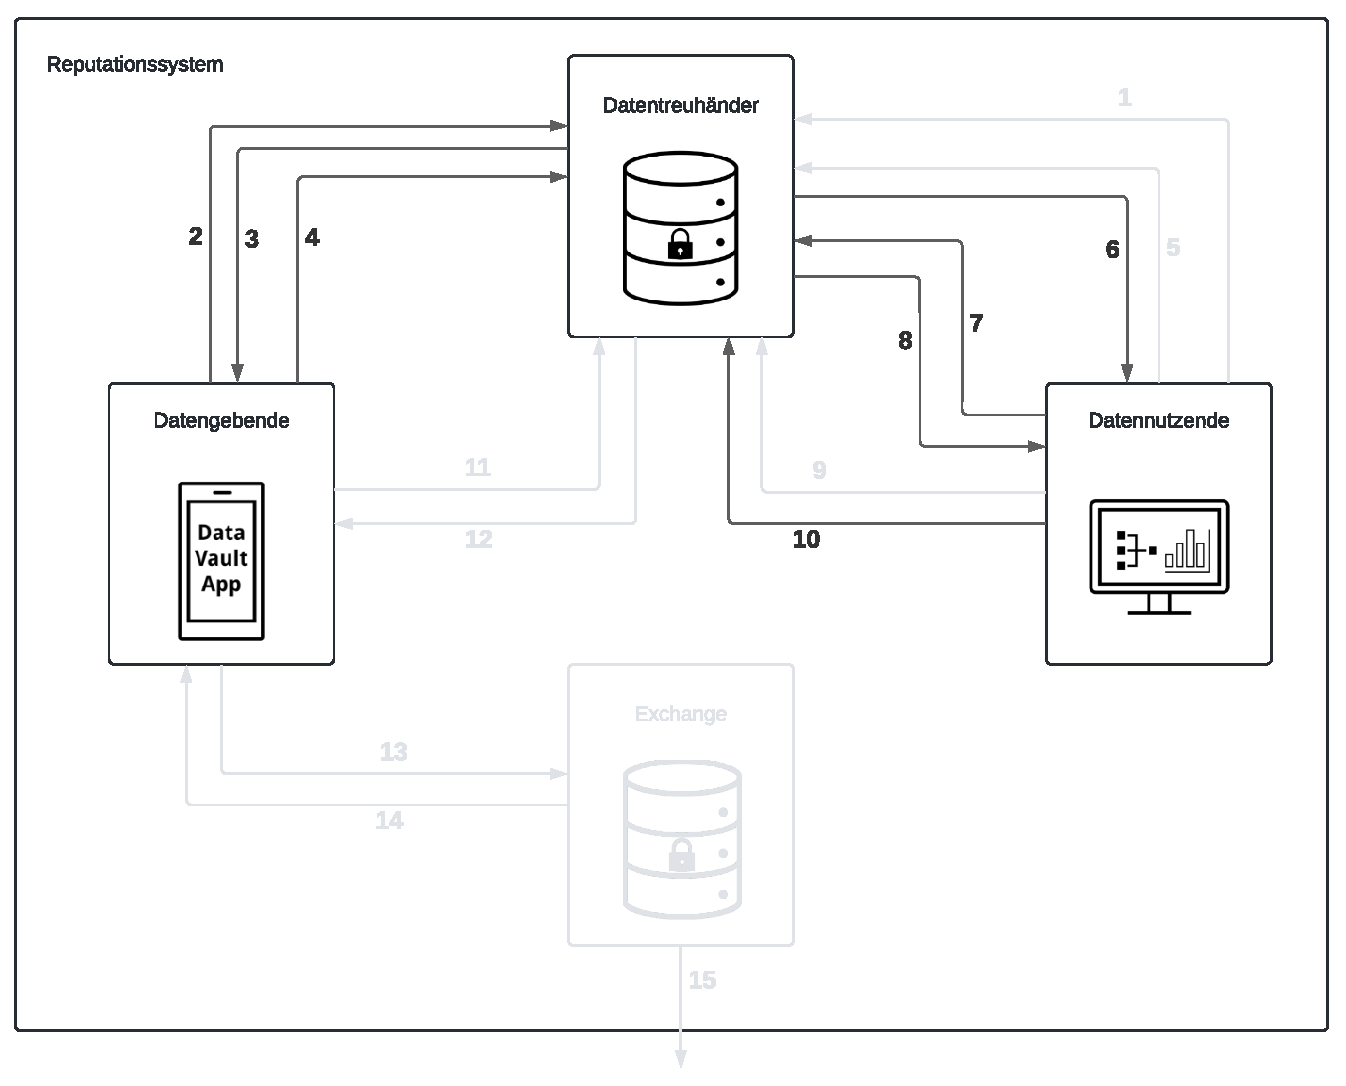
\includegraphics[width=0.9\linewidth]{ReputationDiagramm.pdf}
    \caption{Reputationssystem Ablauf}
    \label{fig:reputation}
\end{figure}

Auch in Abbildung \ref{fig:reputation} werden wieder nur die für das Bewertungssystem relevanten Kommunikationsschritte hervor gehoben. Alle weiteren Schritte sind ausschließlich Teil des Bezahlsystems und in \ref{system:payment} dokumentiert.

\paragraph{4. Bewertungstoken mitsenden}$(RatingToken \leftarrow (nonce, {\{DG-ID\}}_{DT-pk},{\{nonce, {\{DG-ID\}}_{DT-pk}\}}_{DG-sk}))$\\
Beim Teilen von Daten kann ein Datengebender einen Bewertungstoken erstellen. Dafür generiert er zufällig einen $nonce$ der Sicherstellt, dass Bewertungen nicht doppelt eingereicht werden können. Anschließend verwendet er den Public-Key des Datentreuhänders, um damit seine Datengebende ID zu verschlüsseln. Dabei muss ein Saltwert hinzugefügt werden, da sonst beim jedem Verschlüsseln der ID der gleiche Geheimtext entsteht. Dadurch könnte ein Datennutzender den Ursprung von zwei Bewertungstoken verfolgen, was die Privatsphäre der Datengebenden verletzt. Abschließend berechnet der Datengebende eine Signatur über den zufälligen $nonce$ und die verschlüsselte $DG-ID$. Sie stellt sicher, dass ein Datennutzer nicht selbst $nonce$ generiert und mehrere Bewertungs für eine $DG-ID$ einreicht oder die $DG-ID$ nach erhalt des Token ändert. Mit diesen drei Werten ist der Bewertungstoken vollständig und wird zusammen mit der $dataLocation$ und dem $dataKey$ an das Datenpostfach vom Datentreuhänder gesendet. Der Bewertungstoken wird dafür Teil des Strings der mit dem Shared-Key verschlüsselt wird.

\paragraph{6. Bewertungstoken erhalten}$(RatingToken)$\\
Nach der Abfrage des Datenpostfachs in Schritt 5 erhält der Datennutzende die mit dem Shared-Key verschlüsselten Informationen über die Datenspeicherung beim Datentreuhänder, sowie den Bewertungstoken. Aufgrund der im Bewertungstoken übertragenen Details kann der Datennutzende kaum Überprüfungen auf dem Token durchführen. Er kann lediglich den verwendete $nonce$ auf Wiederholungen überprüfen um sicherzustellen, dass er nicht zwei Mal den gleichen Token erhalten hat. Die Signatur von $nonce$ und ${\{DG-ID\}}_{DT-pk}$ benötigt zwar zur Validierung nur den Public-Key des Datengebenden, aber da die $DG-ID$ verschlüsselt ist und im Postfacheintrag der Public-Key des Datengebenden nicht mitgesendet wird, kann der Datengebende den nötigen Public-Key nicht bestimmen. Daher bleibt ihm in diesem Moment nur die Möglichkeit dem Datengebenden und dem überwiesenen Bewertungstoken zu vertrauen und auf die Bewertung des Tokens durch den Datentreuhänder in Schritt 12 zu warten.

\paragraph{7. Reputation abfragen}$({\{DG-ID\}}_{DT-pk})$\\
Den soeben erhaltenen Bewertungstoken kann der Datennutzende verwenden um die darin gespeicherte verschlüsselte Datengebende ID an den Datentreuhänder zu senden. Er selber kann die ID nicht lesen. Da sie mit dem Public-Key des Datentreuhänders verschlüsselt ist, muss sie an ihn weitergeleitet werden um eine Aussage über die Reputation zu treffen. Dieser Schritt muss seperat von den Anfragen der Daten geschehen. Andernfalls weiß der Datentreuhänder, dass die gefragten Daten durch den gleichen Datengebenden hochgelanden wurde, dessen Reputation zurückgegeben werden soll.

Dieser Schritt ist nicht essentiell für das Protokoll und kann bei Bedarf auch weggelassen oder zu einem späteren Zeitpunkt ausgeführt werden. In dem Fall, dass ein Datennutzender keinen großen Wert auf die Korrektheit aller Reputationswerte legt und möglicherweise in seiner Rechenleistung etwas beschränkt ist, kann dieser Schritt und damit zusammen auch Schritt 8 übersprungen werden. Dadurch kann der Datennutzende zwei Kommunikationsschritte sparen. Ein Ansatz, in dem ein Datennutzender nur bei herausstechend schlechten Daten die Reputation des Datengebenden anfragt, ist beispielsweise genauso denkbar.

\paragraph{8. Reputation antwort}$(Reputation)$\\
Der Datentreuhänder kann die Datengebenden ID problemlos entschlüsseln. Anschließend kann er die Reputation des Datengebenden aus seiner Datenbank auslesen und den Wert an den Datennutzenden zurücksenden. Wie der genaue Wertebereich der Reputation definiert ist, hängt von der konkreten Implementation ab. Der empfohlene Bereich ist für eine Reputation $r$ ist $0\leq r\leq 1$. Sollte ein Datengebender das erste Mal abgefragt werden, so kann der Datentreuhänder -- gegebenenfalls, dass die Datengebende ID tatsächlich existiert -- einen neutralen Wert von hier $0,5$ zurück geben. Auf diesem Weg erfährt der Datennutzende die Reputation des Datengebenden, ohne herausfinden zu können, mit welchem Datengebenden er handelt.

\paragraph{11. Bewertung einreichen}$(RatingToken, rating, {\{DN-Certificate\}}_{DT-sk})$\\
Nachdem der Datennutzende eine Bezahlung in das Coinpostfach gesendet hat,hat er die Möglichkeit eine Bewertung für die Qualität der Daten abzugeben. Im Gegensatz zum Übertragen von Coins ist das Abgeben einer Bewertung nicht verpflichtend. Es kann genauso wie Schritt 7 bei durchschnittlicher Qualität der Daten ausgelassen werden um Performanz zu steigern. 

Um eine Bewertung einzureichen sendet der Datennutzende ein Tripel aus dem Bewertungstoken, der Zufriedenheit mit den Daten und einem Datennutzenden-Zertifikat. An dem Bewertungstoken hat sich nichts verändert. Er beinhaltet nach wie vor einen $nonce$, die verschlüsselte Datengebende ID und die Signatur über diese beiden Werte. Nun kann der Datennutzende einen Wert festlegen der seine Zufriedenheit mit den Daten repräsentiert. Dafür muss ein passender Wert aus dem gewählten Intervall bestimmt werden. Für das Datennutzenden-Zertifikat wird angenommen, dass es bei der Registrierung eines Datennutzenden beim Datentreuhänder ausgestellt wird. Es beinhaltet keine Informationen über den jeweiligen Datennutzenden sondern dient in dieser Situation ausschließlich dazu sicherzustellen, dass ein Datengebender sich nicht selbst bewerten kann. 

Das Zertifikat ist optimal durch alternative Beweisformen austauschbar die zeigen, dass es sich bei der bewertenden Person um einen Datennutzenden handelt, ohne dabei anzugeben welcher Datennutzende es ist. Denn wenn der Datentreuhänder bei einer Bewertung den Datennutzenden bestimmen kann, so hat er ein direktes Indiz für den Handel zwischen dem Datennutzenden und dem bewerteten Datengebenden.

Sobald das Tripel beim Datentreuhänder eintrifft überprüft dieser ebenfalls den $nonce$ auf wiederholtes Vorkommen und stellt mit Hilfe des Zertifikates sicher, dass es sich beim dem Bewerter um einen Datennutzenden handelt. Anschließend entschlüsselt er die $DG-ID$, ruft den bekannten Public-Key des entsprechenden Datengebenden ab und nutzt ihn, um die Signatur über den $nonce$ und die verschlüsselte $DG-ID$ zu validieren. Sollten alle diese Überprüfungen ohne Fehler ablaufen so kann der Datentreuhänder sicher sein, dass der Token tatsächlich durch den angegebenen Datengebenden erstellt wurde und ein Datennutzender ihn für die Bewertung von genau diesem Datengebenden benutzt. Er speichert die erhaltene Bewertung zusammen mit der $DG-ID$ lokal bis der Reputationswert des Datengebenden das nächste Mal neu bestimmt wird. Dies kann nach jeder Bewertung, in regelmäßigen Zeitabständen oder beim nächsten Anfragen von Aufrufen geschehen. Dafür kann der Datentreuhänder für jeden Datengebenden dessen aktuelle Reputation und sämtliche Bewertungen seit der letzten Berechnung verwenden, um damit eine neue Reputation zu erhalten. Wie die Gewichtung der unterschiedlichen Bewertungen verläuft ist hier wieder nicht genau vorgegeben. In Abschnitt \ref{chap:impl} wird ein mögliches Beispiel genannt.


\subsection{Weitere Streitfälle}
\label{subsec:repStreit}
Das Reputationssytem bietet weiteres Potenzial für Streitfälle, die durch die hier hinzukommenden Kommunikationsschritte entstehen können. Im folgenden sind diese Streitfälle aufgelistet.
\begin{enumerate}
    \item \textbf{Kein/Doppelter Bewertungstoken.} \label{case:badRepToken}
    Nachdem der Datennutzende in Schritt 6 den Datenpostfacheintrag entschlüsselt hat, prüft er den Bewertungstoken auf Existenz sowie Einzigartigkeit. Sollte dabei auffallen, dass entweder kein Bewertungstoken vorhanden ist oder dieser Token zuvor bereits erhalten wurde, so kann der Datennutzende dieses Verhalten melden. Er liefert dem Datentreuhänder den Shared-Key mit dem er den Datenpostfacheintrag entschlüsseln kann. Stellt der Datentreuhänder ebenfalls einen Fehler mit dem Bewertungstoken fest, so erlaubt er dem Datennutzenden, die Zahlung an den Datengebenden zu unterlassen. Wenn nach Ablauf von 12 Stunden der Datengebende den ``Zahlungszeitraum überschritten`` \ref{case:paymentExceeded} Streitfall meldet, so wird er darauf hingewiesen, dass er keine Zahlung erhalten wird.
    \item \textbf{Zu niedrige Reputation.} \label{case:insufficientRep}
    Wenn dem Datennutzenden nach entschlüsseln des Bewertungstokens und Anfragen der Reputation auffällt, dass der Datengebende nicht dazu berechtigt sein sollte auf den Aufruf zu antworten, legt er wieder den Shared-Key offen. Der Datentreuhänder kann die $DG-ID$ des Datenpostfacheintrags verwenden um zu überprüfen, ob der Datengebende in der Lage sein sollte den Aufruf zu sehen. Ist die Reputation des Datengebenden unter dem Reputationsschwellwert des in dem Datenpostfacheintrag referenzierten Aufrufs, so muss der Datengebende den Aufruf entweder von einer veralteten Aufrufliste haben oder ein anderer Datengebender mit ausreichender Reputation hat eine Liste von aktuellen Aufrufen öffentlich gemacht. Auch hier ist der Datennutzende nicht mehr dazu verpflichtet einen Eintrag in das Coinpostfach einzutragen, da der Datengebende unrechtmäßig einen Aufruf beantwortet hat.
    \item \textbf{Inkorrekte Signatur.} \label{case:badSignature}
    Im Anschluss an das Einreichen einer Bewertung in Schritt 12 wird die Signatur des Bewertungstokens durch den Datentreuhänder überprüft. Sollte dabei ein Fehler entstehen, so wird zuerst der Datennutzende beschuldigt die verschlüsselte $DG-ID$ ersetzt zu haben. Um diese Anschuldigung aufzuklären legt er den Shared-Key offen. Der Datentreuhänder entschlüsselt den Datenpostfacheintrag und prüft, ob die Signatur des übertragenen Token bereits fehlerhaft ist. Stellt sich der übertragene Token als intakt heraus, so hat der Datennutzende versucht die $DG-ID$ des Token zu verändern und so eine Bewertung für einen anderen Datengebenden auszustellen. Dafür kann ihn der Datentreuhänder temporär sperren. Ist der übertragene Token jedoch ebenfalls fehlerhaft, so ist ein Fehler bei der Erstellung der Signatur entstanden. Dieser kann sowohl unwissentlich -- durch das falsche Signieren von korreken Werten -- als auch wissentlich durch das absichtliche Verwenden einer anderen verschlüsselten $DG-ID$ auftreten. Aufgrund dessen kann der Datengebende hinter der $DG-ID$ nicht bestraft werden, da ein anderer Datengebender möglicherweise genau das bezwecken möchte. Daher bleibt wieder nur die Auslassung einer Bezahlung für den Datenpostfacheintrag.
\end{enumerate}

\subsection{Bewertungsfrequenz verschleiern}
\label{sec:ratingObfuscation}
Der Datentreuhänder kennt zwar die Reputation eines jeden Datengebenden, allerdings soll er dessen Handelspartner oder Frequenz nicht anhand der Bewertungen erschließen können. Leider ist dies sehr einfach, da der Datentreuhänder jede Bewertung einem Datengebenden zuordnen muss. Auch wenn nicht jeder Datennutzende eine Bewertung für jeden Handel mit einem Datengebenden ausstellt, lässt sich so für den Datentreuhänder trotzdem ein ungefähres Bild des Engagement eines Datengebenden bilden. Deswegen wird davon ausgegangen, dass es eine Instanz gibt, die sich als Datennutzender beim Datentreuhänder registriert, aber kein Interesse an Daten hat. Sie ist ausschließlich dazu da, um Verschleierungsbewertungen abzugeben. Dafür kann sie einen Aufruf starten wie ein regulärer Datennutzender. Die Datengebenden übertragen jedoch keine Daten an den Datennutzenden sondern lediglich einen Bewertungstoken. Dieser wird dazu verwendet eine Bewertung auszustellen, die mit der aktuellen Reputation übereinstimmt, sodass sich bei Neuberechnung der Reputation kein Unterschied ergibt. Dadurch kann ein Datengebender beliebig viele Bewertungen ausstellen, die seine Reputation nicht verändern und dadurch seine tatsächlich Handelsfrequenz gegenüber dem Datentreuhänder verschleiern. Nun kann der Datentreuhänder beim Erhalt einer Bewertung für einen Datengebenden nicht sicher sein, dass wirklich ein Handel stattgefunden hat, was die Privatsphäre des Datengebenden weiter stärkt.\\

Einige der in den Abschnitten \ref{subsec:payStreit}, \ref{subsec:repStreit} beschriebenen Streitfälle müssen für diesen speziellen Fall anders evaluiert werden. Beispielsweise ist hier der Datengebende im Unrecht wenn er 12 Stunden nach absenden des Tokens den Streitfall \ref{case:paymentExceeded} ausruft, da er keine Daten geteilt hat und somit auch keine Coins erhalten wird.

Bei der Bewertung dieser Streitfälle muss der Datentreuhänder wissen, ob es sich bei dem Datennutzenden um eine solche Verschleierungsinstanz handelt. Dies kompromitiert jedoch nicht die Verschleierung, da die Bewertungen über einen Proxy eingereicht werden und der Datentreuhänder beim Erhalt einer Bewertung nicht weiß, ob sie zur Verschleierung dient oder nicht. Er kann zwar anhand des Datenpostfachs erahnen, wie viele Verschleierungsbewertungen insgesamt abgegeben wurden. Solange die Datengebenden aber in ungleichen Menge Anfragen stellen, kann der Datentreuhänder auch hier durch die Verwendung von Proxys nicht bestimmen woher diese Anfragen stammen.


%==================================================================================================


\chapter{Implementation}
\label{chap:impl}
In dem hier folgenden Kapitel werden einige Details zu der Implementation geklärt, die im Kapitel \ref{chap:auswertung} ausgewertet wird. Dafür wird zuerst das TRESOR-Projekt kurz vorgestellt, einige Änderungen -- die während der Implementation aufkamen -- genannt und alle Parameter für die Wahl von Schlüssellängen und dergleichen begründet.

\section{TRESOR-Projekt}
Um aussagekräftige Testdaten der Entwürfe zu generieren, wurden die in Kapitel \ref{chap:systems} beschriebenen Systeme auf der bereits existierenden Codebasis des TRESOR-Projekts der Universität Hamburg implementiert. TRESOR ist ein C2B-Datentreuhandsystem das darauf abzielt, die in der dazugehörigen Data Vault mobile App eingegebenen oder generierten Daten vorzuverabreiten, zu verschlüsseln und auf Anfrage mit Datennutzenden zu teilen. Die App zielt besonders darauf ab, dem Nutzer volle Transparenz über die Verwendung seiner Daten zu geben. Es ist ein Pilotprojekt an dem eine Reihe an wissenschaftlicher Forschung in Feldern rund um Datentreuhandsysteme, Datenanonymisierung und privatsphärewahrender Datenspeicherung betrieben wird \cite{TRESOR}.

\section{Erweiterungen der Protokolle}
Damit die drei Entwürfe in den bestehenden Code eingebaut und benutzt werden können, mussten zwei Änderungen an den Schritten des Bezahlsystem vorgenommen werden. 
%Die erste Änderungen ist in Schritt 4. Dort überträgt der Datengebende den Speicherort und Schlüssel für das verarbeiten der Daten. Der in diesem Schritt neu erstellte Shared-Key wird zusätzlich mit dem Public-Key des Datennutzenden verschlüsselt, um nur ihm den Zugang zu gewähren. Allerdings kann die geforderte Integrität des ${\{Shared-Key\}}_{DN-pk}$ nur gewährleistet werden, solange der Datengebenden den verschlüsselten Geheimtext mit seinem Private-Key signiert. In dem Datenpostfacheintrag ist allerdings keinerlei Indiz auf die Identität des Datengebenden daher auch nicht auf seinen Public-Key der zum Validieren der Signatur nötig ist. Deswegen wird in der Implementation für jeden von Datengebenden erstellten Datenpostfacheintrag ein neues Schlüsselpaar generiert und mit dessen Private-Key der Geheimtext signiert. Damit der Datennutzende den nötigen Public-Key erhält, wird dieser im Klartext mit in dem Postfacheintrag übertragen. Dadurch wird einem Angreifer ermöglicht, beim Abfangen der Nachricht einen neuen Shared-Key zu generieren, diesen mit einem neuen Schlüsselpaar zu signieren und die Werte der Nachricht mit den neuen Werten für den Shared-Key, die Signatur und den Public-Key ersetzt. Nun kann der Datennutzende die $dataLocation$ und $dataKey$ nicht mehr entschlüsseln, da sich der Shared-Key geändert hat. Meldet er dieses Problem als Streitfall beim Datentreuhänder so überprüft dieser die Nachricht und sieht den Fehler auf der Seite des Datengebenden. 
%Hier ist allerdings zu beachten, dass dieser Angriff nicht erst durch das Hinzufügen der Signatur möglich wird. Wird der Shared-Key überhaupt nicht signiert, so kann ein Angreifer lediglich diesen Austauschen und gelangt zu der selben Auswirkung. ${\{oneTimeECKey\}}_{DG-sk},{\{{\{DG-ID\}}_{DT-pk}\}}_{DN-pk}$
\\

Die zweite Änderung befindet sich in Schritt 5. Hier wurde für eine effiziente Benutzung der Abfrage des Datenpostfachs ein Index hinzugefügt. Dieser hat den Sinn die Antwortgröße minimal zu halten. Wenn bei jeder Abfrage alle Einträge mit Public-Keys des Datennutzenden wiedergegeben werden, so enthält diese Liste nach einiger Zeit zum größten Teil Duplikate, die bereits behandelt wurden. Deswegen überträgt der Datentreuhänder bei jedem Postfacheintrag den Index mit. Dadurch kann ein Datennutzender in seiner nächsten Anfrage einen Index angeben, bis zu welchem er bereits alle Einträge kennt. Der Datentreuhänder kann anschließend nur die Einträge zurückgeben, die einen höheren Index besitzen als der spezifiziere. So bleibt diese in der Regel ähnlich groß anstatt mit der Zeit konstant zu wachsen.

\section{Verwendete Schnittstellen}
Wie bereits erwähnt wurde die Implementation der in Kapitel \ref{chap:systems} beschriebenen Ansätz in dem TRESOR Projekt vorgenommen. Dafür wurden einige bestehende Schnittstellen der Codebasis genutzt. Das TRESOR Projekt befasst sich jedoch hauptsächlich mit den oben beschriebenen Themen von anonymer Datenspeicherungen und Verwaltung, weshalb nur Grundlage für das hier implementierte System bestand. Schnittstellen die verwendet werden konnten, waren in Kapitel \ref{system:payment} Schritt 1, in dem ein Aufruf durch den Datennutzenden gestartet wird, sowie Schritt 2, 3 zum Abfragen sämtlicher Aufrufe. Bei Schritt 2,3 mussten jedoch kleine Änderungen vorgenommen werden, um die Übertragung der Datengebenden ID und die dazugehörige Auswahl an Aufrufen nach Reputation umzusetzen. Die vierte und letzte verwendete Schnittstell in ist Kapitel \ref{system:payment} Schritt 9,10. Sie befasst sich mit dem Abrufen der Daten vom Datentreuhänder die durch einen Datengebenden bereitgestellt wurden.

Alle weiteren Interaktionen zwischen den Akteuren des Protokolls wurden selbst entwickelt, da keine bereits bestehenden Grundlage vorhanden war. 

\section{Parameterwahl}
An dieser Stelle wird die Wahl diverser Parameter der Implementation begründet. Die dafür behandelten Parameter beziehen sich hauptsächlich auf sicherheitskritische Parameter wie Schlüssellänge, Hashfunktionen und Noncelängen.\\
Für eine einheitliche Metrik, die das Sicherheitniveau eines Systems oder Protokoll beschreibt, ist die Verwendung eines Security Bit Levels gängig. Es beschreibt eine untere Grenze für die Anzahl an Operation, die der schnellste bekannte Angriff im Durchschnitt braucht \cite{ecc-hankerson2021nist}. Generell gilt in der Literatur eine Security Bit Level von 128 Bits als ausreichende Sicherheit für die Jahre 2019-2030 und darüber hinaus \cite{elaine2016recommendation}. Selbstverständlich liefert ein höheres Security Bit Level eine höhere Sicherheit gegen Angreifer, die versuchen die Verschlüsselung zu brechen. Allerdings ziehen größere Schlüssellängen auch längere Berechnungszeiten der Ver- und Entschlüsselung mit sich. Es muss also abgewogen werden, ob eine ausreichende Sicherheit mit niedrigen Berechnungszeiten oder eine erhöhte Sicherheit mit erhöhten Rechendauer erreicht werden soll. In der hier vorliegenden Situation spielt eine hohe Sicherheit aufgrund des Handels mit Geld eine große Rolle. Da allerdings gleichzeitig die Anforderungen an Zeitsensitivität besteht, sollte die Rechendauer gering gehalten werden. Deswegen wird in der Implementation ein Security Bit Level von 128 Bit verwendet. Für die asymmetrische elliptische Kurve Krypographie entspricht dies einer Schlüssellänge von mindestens 256 Bits \cite{elaine2016recommendation,bsi2020cryptographic}. Um diesen zu generieren wurde die Kurve $secp256k1$ verwendet, die ein Security Bit Level von 128 Bit aufweist \cite{ecc-duka2020elliptic}. Der symmetrische MAES-Algorithmus ist durch seine Implementation an eine Schlüssellänge von 128 Bits gebunden, was ebenfalls dem Security Bit Level von 128 Bits entspricht \cite{elaine2016recommendation}.\\

Die Sicherheit von Hashfunktionen und deren Kollisionsresistenz kann genauso mit einem Security Bit Level bewertet werden. Sie werden in der Erstellung von Signaturen sowie Hash-based Message Authentication Code (kurz HMAC) -- welche die Integrität bei asymmetrisch verschlüsselten Nachrichten gewährleisten -- verwendet. Die Sicherheit einer Hashfunktion hängt dabei von der Anwendung ab. Beispielsweise hat der SHA-256-Algorithmus für Signaturen Security Bit Level von 128 Bit, während der gleiche Algorithmus für das Erstellen von HMAC ein 256 Bit Security Level erreicht \cite{elaine2016recommendation}. Trotzdessen wird SHA-256 in der Implementation für sowohl das Erstellen von Signaturen als auch von HMAC verwendet.\\

Für die Wahl des CoinGenerationToken Nonce, Coin Nonce und Bewertungstoken Nonce ist ausschlaggebend, dass sich während der Laufzeit des Systems beim kontinuierlich neu Generieren von Werten keine Doppelungen entstehen. Deswegen werden für diese Werte Zufallszahlen mit ebenfalls 128 Bits gewählt, was die Wahrscheinlichkeit eines doppelt vorkommenden Wertes auf $\frac{n}{2^{128}}$ setzt. Dabei ist $n$ die Anzahl an bereits erstellten Nonces für den jeweiligen Verwendungszweck. Eine Wiederholung des gleichen Werts zwei unterschiedlichen Nonces, wie beispielsweise bei einem CoinGenerationToken und einem Coin, hat dabei keine Auswirkungen. Somit braucht es $2^{128}$ Versuche den Nonce zu erraten, was die Vorraussetzung für eine 128 Bit Security Level ist.

\section{Reputationsberechnung}
Die Reputation eines Datengebenden muss regelmäßig neu berechnet werden. Die Berechnung nach jedem Eingang einer neuen Bewertung zu starten ist jedoch unnötig aufwendig. Deswegen wird in der Implementation die Reputation eines Datengebenden bei dessen Nachfrage nach der Aufrufliste gestartet. Dies geht möglichen Verwirrung aus dem Weg die entstehen, falls ein Datengebender an der Schwelle eines Aufrufs ist, diesen Beantwortet und er, bevor der Datennutzende die Reputation überprüft, eine schlechte Bewertung erhält, die ihn unter die Reputationsschwelle treibt.

\begin{figure}[h]
    \centering
    \caption{Verteilung der Gewichte auf den Index}
    \label{fig:reputationWeights}
    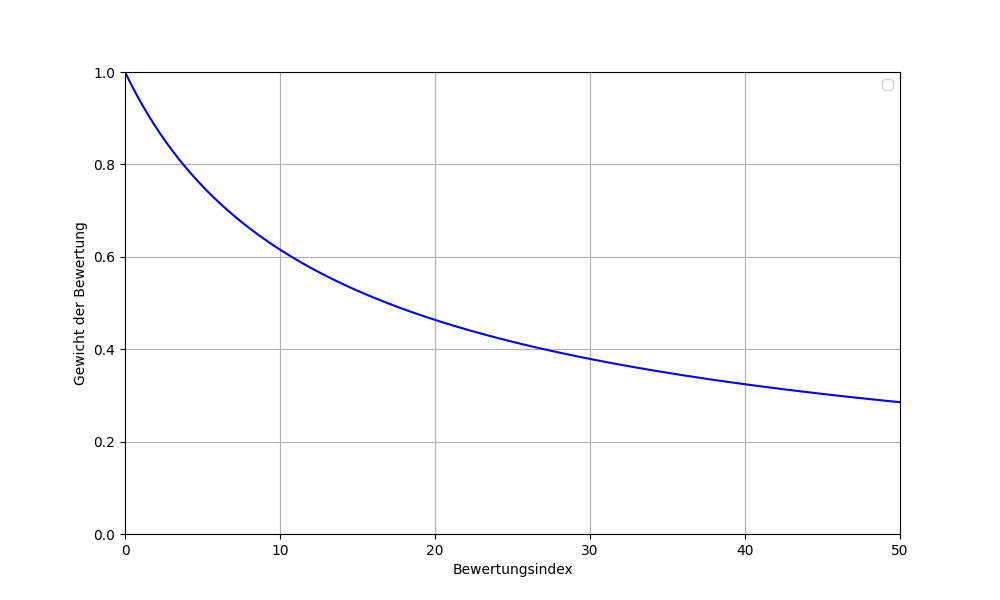
\includegraphics[width=0.8\linewidth]{ReputationWeights.png}
\end{figure}

Für die Neuberechnung werden (soweit vorhanden) die letzen 50 Bewertungen des Datengebenden nach Eingangszeitpunkt absteigend sortiert, sodass die neueste Bewertung an erster Stelle steht. Anschließend werden die Bewertungen mit einem Faktor multipliziert der sich aus der Funktion $f(index)=(0,1\cdot index + 1)^{-0,7}$ ergibt. Der Graph der Funktion ist in Abbildung \ref{fig:reputationWeights} visualisiert. Danach werden alle vervielfachen Bewertungen aufsummiert und durch die Summe der Faktoren geteilt. Die Funktion bevorzugt die neuesten Bewertungen und verleiht ihnen größeren Einfluss auf den entgültigen Reputationswert. Dadurch kann sich ein Nutzer, der in der Vergangenheit viele gute Bewertungen erhalten hat nicht in Sicherheit wiegen sondern wird dazu angereizt, konstant weiter gute Bewertungen zu erhalten.

%schritt 4 braucht auch pk des dg -> für jeden neues keypair erstellen
%schritt 5 hinzufügen von index für benutzbarkeit

%Parameter wahl für alle krypographie wert (schlüssellänge, tokennonce länge, etc)

%Wie wird reputation neu berechnet / wann


%==================================================================================================

\chapter{Evalutation}
\label{chap:auswertung}
Nun da die Formalisierung des Konzepts abgeschlossen ist, kann mit der Auswertung begonnen werden. Dafür wird das Konzept hauptsächlich bezüglich der Sicherheit und des Rechenaufwands analysiert. Für die Analyse der Sicherheit werden die Angreifermodelle aus Kapitel \ref{chap:req} aufgegriffen, weiter spezifiert und anhand von ihnen gezeigt, welche Schwachstellen das Konzept gegen die verschiedenen Angreifer aufweist. Zur Analyse des Rechenaufwands werden gemessene Laufzeiten der Implementation begründet und miteinander verglichen. Später wird zusätzlich geprüft ob die in Kapitel \ref{chap:req} gesetzten Anforderungen erfüllt, sowie antworten auf die in Kapitel \ref{chap:intro} genannten Foschungsfragen besprochen. Zum Schluss gibt es ein Diskussion mit bestehenden Problemen und weiterführenden Ansätzen.
\section{Bewertung der Sicherheit}
\label{sec:auswertungSecurity}
Die Sicherheit eines Systems in Bezug auf verschiedene Angriffe ist ein essenzieller Faktor für den Erfolg dieses Systems. Insbesondere bei kryptographischen Protokollen, wie Keyexchange Protokollen oder dem in Kapitel \ref{chap:systems} präsentierten Bezahlsystem, ist die Sicherheit einer der entscheidenen Punkte die den Erfolg bestimmen können. Um einen Standard für eine Bewertung der Sicherheit einzuführen, definierten D. Dolev und A. Yao im Jahr 1983 das erste Angreifermodell \cite{am-dolev1983security}. Ein Angreifermodell beschreibt einen theoretischen Angreifer, der probiert, dem zu untersuchenden System Schaden zuzufügen oder Informationenen zu extrahieren. Dafür müssen die Rahmenbedingungen des Angreifermodells genau bestimmt werden. Es umfasst in der Regel Angreiferziele, Angreiferannahmen und Angreiferfähigkeiten \cite{am-do2019role}. 
\begin{itemize}
    \item \textbf{Angreiferziele.} Für einen Angreifer gibt es mehrere Ziele, die er mit seinem Angriffen erreichen möchte. Er kann beispielsweise Interesse daran haben, die übertragenen Informationen mitzuschneiden, Geheimnisse wie private oder Sitzungsschlüssel herauszufinden oder die Kommunikation vollständig zu verhindern. 
    \item \textbf{Angreiferannahmen.} Sie beschreiben das Umfeld und die Ressourcen des Angreifers. Häufig auftretende Annahmen sind die Unterscheidung zwischen externem oder internem Zugriff auf ein Netzwerk, die Beschränkung auf einen polynomial probabilistischen Angreifer, was beschreibt dass der Angreifer nur $O(n^k)$ Rechenaufwand bei einem Konstanten $k$ und Eingabelänge $n$ hat und bei der Berechnung zufällige Werte raten darf.
    \item \textbf{Angreiferfähigkeiten.} Die Fähigkeiten eines Angreifers sind durch seine Handlungsmöglichkeiten definiert. So kann ein aktiver Angreifer die Fähigkeiten besitzen, Botnetzwerke zu verwenden um DDoS Attacken zu starten, per Brute Force probieren ein Passwort zu knacken oder Analysen des Geheimtexts durchzuführen, die Schlüsse auf die übertragene Nachricht zulassen. Passive Angreifer hingegen haben meist nur die Möglichkeit, die Kommunikation zu beobachten und Schlüsse aus dem Netzwerkverkehr abzuleiten.
\end{itemize} 
Zusammen ergibt die Definition des Angreifermodells eine maximale Stärke die ein Angreifer besitzen und trotzdessen das System nicht brechen kann. Sollte er in nur wenigen Punkten mehr Macht besitzen als das Angreifermodell vorgibt, so ist die Sicherheit des Systems nicht mehr gewährleistet und der Angreifer kann sein definiertes Ziel erreichen. Daher spricht die Aufstellung eines starken Angreifermodells und die Verteidigung gegen dieses für die Robustheit des Systems. Eine genaue Definition des Angreifermodells ist wichtig, da unpräzise Formulierung ein mehrdeutiges Angreifermodell liefern, das nicht genau bestimmen kann, wogegen das System geschützt ist.

\subsection{Angreifermodelle der Coin Generierungsphase}
\label{subsec:adversaryCoinGen}
Bei einer Durchführung des Coin Generierungsprotokolls treten Exchange und Datennutzende als Akteure auf. Für jeden von ihnen muss ein Angreifermodell definiert werden um die Sicherheit bei korrumpierten Kommunikationteilnehmern zu zeigen. Zusätzlich soll die Sicheheit gegen einen außenstehenden Angreifer gezeigt werden.

\paragraph{Bösartiger Datennutzender}
Ein bösartiges Verhalten eines Datennutzenden kann durch eine Übernahme eines Datennutzenden durch einen externen Angreifer oder durch bösartige Interessen des Datennutzenden selbst entstehen. In beiden Fällen ist das Ziel des Angreifenden, entweder Coins mit größerem monetären Wert zu erhalten als der ursprüngliche Zahlungseingang beim Exchange zulässt oder eine Möglichkeit zu erhalten, selbst Coins zu signieren. Die dafür zu treffenden Annahmen sind, dass es sich um einen aktiven Angreifer handelt. Er verfügt über unbegrenzten Speicher und kann Algorithmen mit polynomieller probabilistischer Rechenzeit ausführen. Zusätzlich kennt er den Public-Key des Exchanges und den für den Zahlungseingang verwendeten $AccountPublicKey (apk)$. Mögliche Angriffe die er starten kann sind Replay-Attacken, welche eine zuvor gesendete Nachricht wiederholen, sowie Chosen-Plaintext-Attack, bei denen der Angreifer den Nachrichteninhalt bestimmt und observieren kann wie sich der Geheimtext verhält, sowie Brute-Force-Attacken zum Erraten des Private-Keys und Geheimtextanalysen zur Herausarbeitung des Private-Keys.\\

Da der Ablauf des Zahlungseingangs in Schritt 1 hauptsächlich von der konkret verwendeten Methode abhängt, kann hier davon ausgegangen werden, dass der Angreifer eine reguläre Transaktion leistet, da er ohne den damit entstehenden $CoinGenerationToken$ das Protokoll nicht vorführen kann. 
Anschließend erfragt er beim Exchange alle Token mit dem verwendeten $apk$. Nach Erhalt des soeben erstellten Token, kann er probieren Coins zu generieren, die den $ES$ Wert des Token übersteigen und den $value$ zusammen mit dem Token zum Exchange zu senden. Da der Exchange zuerst den summierten $value$ Betrag aller Coins mit dem $ES$ des Tokens vergleicht, wird der Exchange bereits hier feststellen, dass ein Angreifer probiert, mehr Geld zu erhalten als er bezahlt hat. Der Versuch schlägt hier fehl.\\

Der Angreifer ist daher gezwungen eine zum $ES$ passende Menge an $values$ zu generieren und zu übertragen. Der Exchange antwortet mit einer Liste von $a,b$ für jeden $value$. Nun kann der Angreifer sich entscheiden das Protokoll für partiell Blinde Signaturen (Abschnitt \ref{sec:partBlindSig}) zu verlassen und anstatt die vorgesehen Berechnung für $e$ auszuführen, $e$ als Variable für den Chose-Plaintext-Angriff zu verwenden. Er schreibt jedem $e$ einen leicht veränderten Wert zu, sendet diesen an den Exchange, erhält für jedes $e$ ein Tupel aus $(r,c,s,d)$ und kann probieren, die Unterschiede zwischen den verschiedenen $r$ mit Hilfe der Geheimtextanalyse herauszuarbeiten. \todo{Faktorisierungsproblem mit großen Primzahlen referenzieren} Da der Exchange zur Berechnung von $r$ zwei dem Angreifer unbekannte Variablen benutzt ($u,x$) und auf das Ergebnis $mod$ $q$ anwendet, ist bei einer ausreichend großen Wahl von $u,x,q$ anzunehmen, dass das Ergebnis pseudozufällig erscheint und keine Hinweise auf $x$ liefert. Dabei verliert der Angreifer zusätzlich bei jedem Versuch den Wert des Coins, da die entstehende Signatur nicht gültig ist.\\

Sollte der Angreifer $e$, wie vom Protokoll vorgesehen, berechnen und nach Erhalt von $(r,c,s,d)$ probieren $u,x$ zu erraten, sodass die Ergebnisse seiner Berechnung mit $(r,c,s,d)$ übereinstimmen, kann er diesen Brute-Force-Angriff ohne Kosten (abgesehen von Rechenaufwand) starten. Solange $q$ groß genug gewählt ist (in der Implementierung 128bits) mit $u{\in}_{R} {\mathbb{Z}}_{q}$ ist die Chance allein $u$ korrekt zu bestimmen bereits $\frac{1}{2^{128}} \approx \frac{1}{3,4\cdot10^{38}}$ ausreichend gering, um das Gelingen des Erratens von $u$ und $x$ als vernachlässigbar anzunehmen.

Der Angreifer kann auch probieren, anhand des Public-Keys des Exchange einen Faktorisierungsalgorithmus laufen zu lassen, um den Private-Key zu bestimmen. Noch sind aber keine Algorithmen bekannt, die das Faktorisierungsproblem in aufbringbarer Zeit effizient lösen können, weshalb der Angreifer auch mit diesem Vorgehen nicht an den Private-Key kommt.\todo{proof}\\

Nach Ausstellung der Signatur ist der Wert jedes Coins fest zugeteilt. Wenn ein Angreifer versucht den $value$ des signierten Coins zu ändern, werden damit die Grundlagen zum Überprüfen der Signatur umdefiniert, was dazu führt, dass jede Validierung fehlschlägt. Somit verliert der Coin schlagartig seinen Wert sobald der Angreifer den $value$ verändert.\\

Letztlich kann der Angreifer probieren einen Replay-Angriff zu starten und einen bereits einmal eingesetzten $CoinGenerationToken$ erneut mit einer Reihen an $values$ zum Exchange zu senden. Jedoch ist in Kapitel \ref{system:coingeneration} definiert, dass der Exchange jeden erhaltenen $CoinGenerationToken$ auf eine doppelte Einlösung überprüft. Daher wird der Exchange die Annahme des Tokens verweigern und der Angreifer schafft es auch hier nicht, mehr Coins zu erhalten als ihm zustehen.\\

\paragraph{Neugieriger Exchange.}
Der Exchange stellt in der Coin Generierungsphase eine Rolle mit großer Verantwortung da. Er hat die Aufgabe Geldsummen sicher zu verwalten und trotz der Anonymität des Konzeptes genau die passenden Mengen ein- und auszuzahlen. Trotzdem wird das Angreifermodell für den Exchange hier nur schwach definiert. Dies hat vor allem den Hintergrund, dass das Konzept eines Exchanges zum Tausch von Geld in die jeweilige Kryptowährung bereits etabliert ist und viele Sicherheitsmaßnahmen bestehen, die den Exchange zu einem gutmütigen Verhalten zwingen \cite{gnu-burdges2016enabling,kim2018risk,baum2021p2dex}. Deswegen wird im Folgenden nur die Sicherheit des Protokolls gezeigt aber nicht die Sicherheit des Exchanges.
Angenommen der Exchange kann nicht durch Unbefugte übernommen werden, so sind seine Angreiferziele in Erfahrung zu bringen, welcher Datennutzende wie viele Coins besitzt und wie viel diese Wert sind. Zusätzlich ist er daran interessiert herauszufinden, mit wem der Datennutzende der sich die Coins signieren lässt, handelt. Dafür möchte er sowohl die Identität des Datennutzenden als auch des Coins wiedererkennen können und verschiedene Signiervorgänge untereinander verlinken können. Die Angreiferannahmen beschränken sich zum größten Teil auf passives Verhalten. Er hält sich überwiegend an das Protokoll und beobachtet die Kommunikation mit dem Datennutzenden, um daraus Informationen zu sammeln. Seine Rechenleistung ist polynomial probabilistisch und er kennt sämtliche Informationen die im ersten Schritt angegeben werden. Die Angreiferfähigkeiten sind ebenso eingeschränkt. In den meisten Fällen antwortet er auf Anfragen des Datennutzenden wie das Protokoll es vorgibt. Nur die Wahl der Berechnungswerte für die partiell blinden Signatur kann er variieren.\\

Wie bereits definiert hält sich der Exchange zunächst an das Protokoll. Er erstellt beim Eintrefen einer Zahlung einen $CoinGenerationToken$ mit dem $ES$ und $apk$ gleich den Werten der Zahlung und legt diesen mit dem $apk$ verschlüsselt in seinem Speicher ab. Da der $apk$ ein regulärer Public-Key ist, kann der Exchange keine fundierten Kenntnissen aus einem $apk$ ziehen. Erst sobald der selbe $apk$ für eine spätere Zahlung erneut angegeben wird, kann davon ausgegangen werden, dass der Zahlungseingang von der gleichen Person stammt. Wenn ein Datennutzender aber für jede Zahlung einen neuen $apk$ generiert, kann der Exchange zwei verschiede Zahlungen nicht zu der gleichen Person zurückführen.

Auf Anfrage gibt er den $CoinGenerationToken$ heraus. Bei dem Berechnen der partiell blinden Signatur ist der einzige Wert, für den eine Abweichung vom Protokoll sinnvoll sein kann, der Private-Key. Die Werte $u,s,d,z,c,r$ sind bei jedem signierten Coin unterschiedlich. Diese gleich zu behalten würde ab dem zweiten Coin dem Datennutzenden auffallen. Der Private-Key hingegen ist dem Datennutzenden nicht bekannt und die Auswirkung beim auswechseln des Private-Keys sind nicht feststellbar. Daher kann der Exchange probieren, für jeden signierten Coin einen eigenen Private-Key zu verwenden. Dadurch kann er beim späteren Erhalt von Coins im Bezahlsystem durch den Datengebenden nachvollziehen, aus welcher Signieranfrage der Coin stammt und kann so die Beziehung zwischen dem Datennutzenden und Datengebenden vermuten. An dieser Stelle greift jedoch der $BDLEQ$, welcher in \ref{sec:privacy-pass} erklärt wurde und verhindert, dass der Exchange unbemerkt den Private-Key austauschen kann. Bei einem Versuch den Private-Key zu ersetzen, zeigt der $BDLEQ$, dass der verwendete Private-Key nicht mehr mit dem beworbenen übereinstimmt. Somit ist der Exchange gezwungen den gleichen Private-Key einzusetzen, was die potenzielle Wiedererkennung im späteren Verlauf verhindert. Somit ist der Exchange gezwungen den selben Private-Key für alle Signieranfragen zu verwenden, was seine Informationsgewinnung erheblich einschränkt.\\

Da für das Anfragen einer Signatur der Coin partiell geblendet wird, ist nur dessen $value$ für den Exchange sichtbar. Der $nonce$ der dem Coin seine Identität verleiht, bleibt vor dem Exchange vorerst versteckt. Daher hilft einen Exchange der bei einem Signiervorgang erhaltene $nonce$ nicht dabei, den selben Coin beim Einlösen wiederzuerkennen. In Kapitel \ref{system:coingeneration} wird zusätzlich vorrausgesetzt, dass der $value$ des Coins aus einer kleinen Mengen an möglichen Werten ausgewählt sein muss. Wenn sich ein Datennutzender nicht an diese Vorschrift hält und einen Coin mit beispielsweise $123,45$\texteuro\ signieren lassen will, kann sich der Exchange diesen $value$ merken. Wenn dieser Betrag so einzigartig ist, dass ihn kein anderer Datennutzender ebenfalls benutzt hat, so kann der Exchange beim Einlösen eines Coins mit dem $value = 123,45$\texteuro\ sicher sein, dass der Datengebende diesen Coin im Handel mit dem Datennutzenden erhalten hat, dessen $apk$ er sich gemerkt hat. Solange jedoch jeder Datennutzende die $values$ seiner Coins aus der Mengen an möglichen Werten auswählt, gibt es für jeden $value$ ein großen Anzahl an Vorkommnissen, die es dem Exchange unmöglich macht mit Sicherheit einen eingelösten Coin zu einer Signieranfrage zu verlinken.

Daher bleibt dem Exchange keine Möglichkeit die Identität eines Datennutzenden über mehrere Signieranfragen zu verlinken, solange er für jede Anfrage einen neuen $apk$ verwendet. Des Weiteren muss der Exchange die Coins mit dem gleichen Private-Key signieren was eine Verlinkung über verschieden Private-Keys ausschließt und kann anhand des $values$ keine Zusammenhänge zwischen Signier- und Einlösephase treffen. Zusammen bedeuted dies, dass er seine Angreiferziele nicht erreicht.

\paragraph{Außenstehender Angreifer.} Der außenstehende Angreifender wurde bereits in dem Kapitel \ref{chap:req} kurz dargelegt. Seine Ziele sind es -- bezogen auf die Coin Generierungsphase -- selbst die Coins zu erhalten, für die der Datennutzende gezahlt hat. Zusätzlich möchte er den Datennutzenden davon abhalten, seine Coins zu erhalten und die Möglichekeit besitzen, einen Datennutzenden anhand von zwei Signieranfragen wiederzuerkennen. Die Annahmen über den außenstehenden Angreifender sind die Folgenden. Er ist ein externer Angreifer und daher kein vorgesehener Teilnehmer der Kommunikation. Er kennt den in Schritt 1 verwendeten $apk$ des Datennutzenden, hat aber kein Wissen über den dazu gehörigen Private-Key. Zu dem hat er unbegrenzten Speicherplatz und verfügt über Algorithmen mit polynomieller Laufzeit. Seine Fähigkeiten umfassen das Ausführen von Brute Force Angriffen, Geheimtextanalysen und Replayangriffen. Außerdem kann er sämtliche Nachrichten die während der Protokollausführung gesendet werden mitschneiden und selbst die Kommunikation zum Exchange aufnehmen. Ein Man in the Middle Angriff ist jedoch nicht möglich.\\

Angenommen der Angreifer hat die erste Nachricht mit dem Eingang der Zahlung und dem $apk$ mitgeschnitten, so hat er die Informationen über sowohl die erhaltenen Summe $ES$ als auch den $apk$. Da der in Schritt 2 übertragene $CoinGenerationToken$ mit dem $apk$ verschlüsselt ist, kann er die Nachricht nicht in realistischer Zeit entschlüsseln, da kein polynomieller Algorithmus bekannt ist, der ECC ohne Kenntnisse über den Private-Key entschlüsseln kann. Ihm bleibt übrig nachdem er die Nachricht mitgeschnitten hat, durch Brute Force zu versuchen den $nonce$ zu erraten, den daraus entstehenden Token mit dem $apk$ zu verschlüsseln und zu prüfen, ob das entstehenden Ergebnis sich mit dem mitgeschnittenen Token deckt. Allerdings ist einerseits der $nonce$ 128 Bit lang was bedeutet, dass er $2^{128}$ Möglichkeit durchprobieren muss, um den richtigen Wert zu finden. Andererseits hat dafür nur solange Zeit, wie der Datennutzende zum Erstellen der Coins braucht, da nach abgeschlossener Signtatur der Coins, der Token als benutzt gespeichert wird. Der Angreifer kann probieren nach dem Mitschneiden der ersten Nachricht für alle möglichen $nonce$ den entsprechenden Token zu verschlüsseln und in einer Hashmap mit Zugriffszeit $O(1)$ abzulegen. Sollte es ihm gelingen alle $2^{128}$ mögliche Token zu Erstellen und Verschlüsseln bevor der Datennutzende seinen $CoinGenerationToken$ beim Exchange anfragt, so kann ein Rennen zwischen Angreifer und Datennutzenden entstehen, in dem der gewinnt, der zuerst seine Coins mit dem Token zum Exchange sendet. Solange aber von einer ähnlichen Berechnungszeit wie in \cite{nofriansyah2018efficiency} ausgegangen wird, braucht der Angreifer $0,02 \cdot 2^{128}\approx 6,8\cdot10^{36}$ Sekunden oder $2,16\cdot10^{29}$ Jahre um diese vollständige Hashmap an Token anzulegen. Daher kann davon ausgegangen werden, dass der Angreifer nicht an den lesbaren $CoinGenerationToken$ kommt, bevor der Datennutzende diesen Verwendet.\\

Die anschließenden Schritte welche die für die partiell blinden Signaturen nötigen Daten austauschen sind ebenfalls alle mit dem $apk$ beziehungsweise mit dem Public-Key des Exchanges verschlüsselt, weshalb der Angreifer den passenden Private-Key bestimmen müsste, um den Verkehr mitzulesen. Da es auch hier keinen Algorithmus gibt, der dies in polynomieller Zeit schafft, kann angenommen werden, dass der Angreifer die Nachrichten nicht lesen kann. Somit erhält er keinen Zugang zu den vom Datennutzenden generierten Coins. Auch die Identität des Datennutzende kann nicht mit einer anderen Signieranfrage verlinken, solange der Datennutzende für jede Anfrage einen neuen $apk$ verwendet.

Um den Datennutzenden vom Erhalt seiner Coins abzuhalten, fehlen in die jegliche Fähigkeiten. Er kann zwar alle Nachrichten die gesendet werden mitschneiden, kann aber die Übertragung nicht stören oder Nachrichten verschwinden lassen. Würden die Angreiferfähigkeiten auf das verschwinden lassen von Nachrichten ausgeweitet werden, könnte er jede Nachricht des Protokoll wiederholt löschen und somit die Kommunikation vollständig verhindern. Der einzige Wege auf dem er den Datennutzenden sonst vom Erhalt seiner Coins abhalten kann, ist den $CoinGenerationToken$ vor dem Datennutzenden auszugeben, was wie gerade erklärt sehr unwahrscheinlich ist.

Der Angreifer kann versuchen Coins zu erhalten, für die er nicht gezahlt hat. Angenommen er schafft es mit einer Geheimtextanalyse über die Unterschiede zwischen dem in Schritt 2 und in Schritt 4 übertragenen Token den Klartext des $CoinGenerationTokens$ zu bestimmen. Dann kann er probieren eine Interaktion mit dem Exchange ab Schritt 4 zu starten und den Klartext des Token mit in die Anfrage zu senden. Dieser Versuch wird jedoch fehl schlagen, da der analysierte Token bereits beim Exchange eingelöst wurde und dieser ihn als $spent\leftarrow true$ gespeichert hat, was weitere Verwendungen des Tokens unterbindet. Der außenstehende Angreifer erreicht daher keines seiner Ziele.

\subsection{Angreifermodelle der Bezahlphase}
\label{subsec:adversaryPayment}
In der Bezahlphase des Systems steigt die Anzahl der Beteiligten im Vergleich zur Coin Generierungsphase um das Dopplte. Somit müssen für die Bewertung der Sicherheit des Bezahlsystems vier Angreifermodelle für die Beteiligten und ein zusätzliches für außenstehende Angreifer erstellt werden. Daraus ergeben sich insgesamt fünf Angreifermodelle gegen die die Sicherheit des Systems im Folgenden geprüft wird.

Vorab kann hier zusammengefasst werden, dass alle Angreifermodelle über unbegrenzten Speicherplatz verfügen und für das Ausführen jeglichen Angriffe nur Zugriff auf Algorithmen mit polynomieller Laufzeit haben.


\paragraph{Neugierig aber ehrlicher Datentreuhänder.}
Kapitel \ref{chap:basics} beschreibt, dass die Rolle des Datentreuhänders in der Verwaltung sowie Verbreitung der mit ihm geteilten Daten eine essentielle Rolle spielt.  Er ist dazu verpflichtet im Sinne des Datengebenden zu handeln weshalb hier nur von einem passiven Angreifer ausgegangen wird. Seine Ziele sind es anhand der über ihn kommunizierten Daten herauszufinden, wie viel ein bestimmter Datengebender handelt und mit welchem Datennutzender er diese Handel eingeht. Der neugierig aber ehrliche Datentreuhänder ist ein passiver Angreifer weshalb er an die genaue Ausführung des Protokollablaufs gebunden ist. Er darf diesen nicht verlassen, sondern kann nur über ihn übertragenene Daten mitschneiden. Seine Angreiferfähigkeiten umfassen die Informationsgewinnung aus erhaltenen Nachrichten, mögliche Geheimtextanalysen auf ihnen. Zusätzlich kann der neugierig Datentreuhänder mit bösaritgen Datennutzenden zusammenarbeiten und zu einem beliebige Zeitpunkt nachfragen, welche Informationen der Datennutzende bis zu diesem Zeitpunkt erhalten hat.\\

Das Erstellen eines Aufrufs in Schritt 1 des Bezahlsystemprotokolls in Kapitel \ref{system:payment} ist für das Erreichen der Angreiferziele uninteressant, da hier nur Informationen über den Datennutzenden bekannt werden. Da sich die Ziele jedoch nur auf Informationsgewinnung über den Datengebenden beziehen, kann dieser Schritt hier ohne weitere Beachtung gelassen werden. 

In Schritt 2 hingegen baut der Datengebende das erste Mal eine Verbindung auf. Er überträgt seine Datengebenden ID an den Datentreuhänder, der mit dieser die genaue Identität des Datengebenden bestimmen kann und alle Aufrufe herausfiltern, die der Reputation des Datengebenden entsprechen. Der Datentreuhänder weiß nun, dass der Datengebende eine aktuelle Version der Aufrufliste besitzt. Diese Information hilft ihm allerdings nicht, da der folgenden Schritt 4 über einen Proxy mit TLS gesendet wird. So kann der Datentreuhänder zwar die Integrität der Nachricht sicherstellen, kann aber nicht herausfinden wer die Nachricht gesendet hat. Die erhaltenen Daten umfassen keine Informationen die auf die Identität des Datengebenden schließen lasse. Daher bringt selbst -- nachdem der Datennutzende in Schritt 6 die Daten erhalten und entschlüsselt hat -- eine Nachfrage des Klartext der verschlüsselten Nachricht den Datentreuhänder nicht näher an Ziel. Dies gilt allerdings nur, solange wie in Abschnitt \ref{sec:systemAssumptions} angenommen wurde, der Datentreuhänder selbst nicht bestimmen kann, von welchem Datengebenden die an der $dataLocation$ angelegten Daten stammen.

Schritt 9 legt nur die $dataLocation$ offen, welche der neugierig Datentreuhänder nach einer Anfrage des Klartexts bereits weiß. Er lernt daher auch durch Schritt 9,10 keine wichtigen neuen Informationen über den Datengebenden. In Schritt 11 überträgt der Datennutzende die Coins für die Bezahlung zusammen mit dem $referenceCode$ an den Datentreuhänder. Der $referenceCode$ ist eine, für jeden Datenpostfacheintrag neu generierte Zahl die keine Informationen des Datengebenden beinhaltet. Die Coins stammen vom Datennutzenden der diese selbst erstellt hat. Das Wissen über diese Nachrichteninhalte kann er beim Datennutzenden erfragen. Es hilft ihm aber nicht Indizien über die Identität des Datengebenden zu finden.\\

Da der Datengebende zum Abholen seiner verschlüsselten Coins aus dem Coinpostfach wieder einen Proxy mit TLS verwendet, weiß der Datentreuhänder nur, dass jemand die Coins zu dem $referenceCode$ abgefragt hat. Alle weiteren Daten über mögliche Public-Keys des Anfragen oder dessen Datengebenden ID bleiben geheim. Da die Coins mit Shared-Key verschlüsselt sind kann der Datentreuhänder davon ausgehen, dass die Coins von der gleichen Person abgefragt wurde, die den Datenpostfacheintrag in Schritt 4 gesendet hat. Er kann also den Eingang eines Datenpostfacheintrag und die Anfrage des Coinpostfach verlinken. Jedoch kann er aus dieser Verlinkung keinerlei Wissen über den Datengebenden ziehen. Weil alle Postfachanfragen seitens Datengebenden über Proxys ablaufen kann der liefert die IP-Adresse keine Hinweise auf die Identität. Die Benutzung von TLS stellt sicheer, dass der Public-Key des Datengebenden nicht für die Anfragen der Postfächer verwendet wird, weshalb der Datentreuhänder auch hier nichts über den Datengebenden lernt. Da der Datentreuhänder keinen Datengebenden eindeutig bestimmen kann, kann er auch keine Aussage über die Handelsfrequenz eines Datengebenden treffen.\\

Die Anschließenden Schritte geschehen nur noch zwischen dem Datengebende und dem Exchange, sodass weder der Datentreuhänder noch der Datennutzende involviert sind. Somit erreicht der neugierig aber ehrliche Datentreuhänder sein Ziel Informationen den Datengebenden und dessen Handelspartner zu gewinnen nicht, da er zu keinem Zeitpunkt weiß, welcher Datengebende mit dem Datennutzenden kommuniziert.

\paragraph{Bösartiger Datennutzender.}
Wie schon in Kapitel \ref{chap:req} erwähnt wurde, sind die Ziele eines bösartigen Datennutzenden, herauszufinden von welchem Datengebenden die erhaltenen Daten stammen. Des Weiteren liegt es in seinem Interesse für den Erhalt von Daten keine Coins ausgeben zu müssen. Das Dritte seiner Ziele ist es den Datengebenden mit Hilfe des Streitfallsystems unrechtmäßig durch den Datentreuhänder bestrafen zu lassen. Dazu sei gesagt, dass in den meisten Streitfällen bei bewiesener Unschuld des Datennutzenden, ein Ausbleiben der Zahlung die Konsequnz ist und daher die letzen beiden Ziele Hand in Hand gehen. Bei dem bösaritgen Datennutzenden handelt es sich um einen internen Angreifer, der in die direkte Kommunikation mit dem Datentreuhänder verwickelt ist. Die erste Angreiferfähigkeit des bösaritgen Datennutzenden besteht in der Kooperation mit einem neugierig aber ehrlichen Datentreuhänder -- wie bereits im letzten Absatz. Er kann zu jedem Zeitpunkt von dem vorgegebenen Protokoll abweichen und beliebige Nachrichten senden.\\

Zuerst beginnt der Datennutzenden in Protokollschritt 1 damit einen Aufruf zu Erstellen. Hier kann bereits probieren den ersten Streitfall aufzusetzen. Dafür gibt er dem Aufruf einen beliebigen Public-Key, dessen zugehöriger Private-Key ihm nicht bekannt ist und sendet diesen Aufruf beim Datentreuhänder. Nachdem der Datengebende den Aufruf angefragt und einen entsprechenden Datenpostfacheintrag gesendet hat, kann der Datennutzende diesen beim Datentreuhänder anfragen. Da er einen Public-Key angegeben, dessen über Gegenstück er nicht verfügt, kann er den Shared-Key nicht entschlüsseln. Er meldet deswegen einen Fehlerhaft Verschlüsselungs Streitfall aus Abschnit \ref{case:IncorrectEncryption}. Wie dort beschrieben ist, wird nach Ablauf des maximal Bezahlzeitraums eine Beschwerde des Datengebenden eingehen, der nach dem Verbleib seiner Coins fragt. Dieser wird dazu aufgefordert den Shared-Key mit dem Datentreuhänder zu kommunizieren. Nachdem der Datentreuhänder den Shared-Key mit dem angegebenen Public-Key des Aufrufs verschlüsselt hat und sich die Ergebnisse mit dem Datenpostfacheintrag decken, fällt auf, dass der Datennutzende entweder den Shared-Key entschlüsseln kann oder einen falschen Public-Key angegeben hat. In beiden Fällen wird hier der Datennutzende bestraft. Auch aus der Zusammenarbeit mit dem neugierigen Datentreuhänder lernt er nichts über den Datengebenden solange dieser für die Klärung des Streitfalls weiterhin einen Proxy, sowie TLS verwendet.\\

Angenommen der Datennutzende hätte in Schritt 1 einen gültigen Public-Key angegeben zu dem er einen Private-Key besitzt, dann kann er in Schritt 9 die Daten der $dataLocation$ abfragen und diese nach dem Erhalt in Schritt 10 entschlüsseln. Meldet er nun den Streitfall Fehlerhafte Datenparameter, so kann der Datennutzende den Shared-Key zum Datentreuhänder senden, welcher den damit den Datenpostfacheintrag einschlüsselt,  die $dataLocation$ abfragt und die dort liegenden Daten mit dem $dataKey$ entschlüsselt. Da der Datengebende sich hier gutartig verhält, wird der Datentreuhänder feststellen, dass der Datennutzende die Daten lesen konnte. Somit wird wieder der Datennutzende bestraft aber nicht der Datengebende. Beim bewerten des Steitfalls lernt der Datentreuhänder die gleichen Informationen wie der Datennutzende, weshalb aus der Zusammenarbeit mit ihm keine neuen Informationen über den Datengebenden zum voschein kommen. \\

Versucht der Datennutzende trotz qualitativ hochweritger Daten den Streitfall Nutzlose Daten auszulösen, so wird die Überprüfung genauso abgehandelt wie im letzten Absatz. Dabei stellt sich wieder heraus, dass der Datennutzende betrügen wollte. Es werden weiterhin keine Details bezüglich des Datengebenden preisgegeben.\\

Der nächste Ansatzpunkt ist in Schritt 11. Hier kann der Datennutzende zuerst probieren keine Coins zu übertragen. Da die gesamte Nachricht in der sich die Coins befinden verschlüsselt ist, sieht der Datentreuhänder nicht ob Coins enthalten sind. Erst nach Schritt 14 in dem der Datengebende die Nachricht entschlüsselt hat, kann er den Streitfall Fehlerhafte Coins auslösen und den Shared-Key sowie den $referenceCode$ zum Datentreuhänder senden. Nun kann dieser die Nachricht entschlüsseln. Da er keine Coins vorfindet wird der Datennutzende bestraft. Das gleiche Verhalten kann in dem Fall angewendet werden, dass der Datennutzende zu wenig Coins überträgt. Wenn der Datengebende zusätzlich einen Verweis auf den Datenpostfacheintrag mitsendet, so kann der Datentreuhänder den Aufruf bestimmen und den Preis dessen mit dem Wert der erhaltenen Coins abgleichen. Um für Daten nicht zu bezahlen kann der Datennutzende ebenfalls versuchen, selbst einen Coin zu erstellen und diesen zu übertragen. Nachdem der Datengebende die Nachricht mit dem selbst erstellten Coin entschlüsselt hat, schlägt das Prüfen der Signatur fehl, voraufhin er den gleich Streitfall auslöst und die gleiche Schlichtung geschieht. Als dritte Möglichkeit kann ein Datennutzender probieren, den gleichen Coin an mehrere Datengebende zu bezahlen. Dieses Verhalt wird erst nach Schritt 16 erkannt. Beim Einlösen des Coins bei einem Exchange fällt auf, dass der Coin bereits vorher von einem anderen Datengebenden ausgegeben wurde. Deswegen stellt der Exchange wie in Schritt 16 beschrieben eine signierte Antwortnachticht aus die belegt, dass der Coin von einem Datennutzenden doppelt ausgegeben wurde. Nun kann der Datengebende mit dieser Nachricht, dem Shared-Key und dem $referenceCode$ zum Datentreuhänder gehen, welcher nach einer Analyse des Beweismaterials wieder den Datennutzenden bestraft. Dem Datennutzenden bleibt also nichts anderes übrig, außer dem Datengebenden eine korrekte Menge an signierten Coins zu bezahlen, die noch nicht ausgegeben wurden.\\

Zum lösen der Streifälle wird wieder nur der Shared-Key, der $referenceCode$ und gegebenenfalls die Nachricht des Exchanges benötigt. Die ersten beiden sind wie schon erwähnt zufällig. Die Nachricht des Exchanges gibt keine Informationen über den Datengebenden. Da der Exchange die signierte Datengebenden ID beim einlösen erhält, kann er mit Sicherheit sagen, dass die Coins von einem anderen Datengebenden eingelöst wurden. Welcher andere Datengebende dies ist, behält er für sich. Nach Schritt 11 sind alle Interaktionen des Datennutzenden innerhalb des Protokolls abgeschlossen. Er hat es weder geschafft Informationen über den Datengebenden herauszufinden, noch den Datengebenden unrechtmäßig zu bestrafen und wurde dazu gezwungen die korrekte Menge an Coins zu bezahlen. Er hat also keines seiner Ziele erreicht.

\paragraph{Bösartiger Datengebender.}
Das Angreifermodell eines bösartige Datennutzenden wurden bereits in Kapitel \ref{chap:req} kurz genannt. Ein bösartiger Datennutzender verfolgt eine Liste an Angreiferzielen. Das erste Ziel ist es ohne Daten an Coins des Datennutzenden zu gelangen. Er will in der Lage sein, Coins von anderen Datengebenden zu stehlen und selbst einzulösen. Zusätzlich möchte er den Datennutzenden durch das Streitfallsystem unrechtmäßig bestrafen lassen. Bei einem bösartigen Datennutzenden handelt es sich um einen aktiven Angreifer der Nachrichten sendet und von dem definierten Protokoll nach belieben abweichen kann. Er ist intern in die Kommunikation eingebunden da er direkt mit dem Datentreuhänder und dem Exchange kommuniziert. Die Angreiferfähigkeiten eines bösaritgen Datengebenden sind das Ausführen von Brute Force Angriffen und das Erstellen einer Geheimtextanalyse.

Zu Beginn in Protokollschritt 2 ist der Datengebende dazu gezwungen seine eigende ID anzugeben, da beim angeben einer anderen Datengebenden ID die Signatur nicht mehr stimmt. Somit ist sichergestellt, dass ein Datengebender nur die Aufrufe für seine Reputation anfragen kann. Daraufhin erhält den Datengebenden eine Liste an Aufrufen aus denen er sich einen aussucht. Da er dem Datennutzenden keine Daten zur Verfügung stellen möchte, kann er nun entweder eine fälschliche $dataLocation$ angeben, die auf leeren Speicherplatz beim Datentreuhänder zeigt oder einen fälschlichen $dataKey$ der die Daten der $dataLocation$ nicht entschlüsseln kann. Natürlich kann er auch beides gleichzeitig verwenden. Die inkorrekten Daten verschlüsselt er nun mit dem neu generierten Shared-Key und sendet sie an das Datenpostfach des Treuhänders. Da der Datennutzende die Daten nach dem Anfragen und entschlüsseln nicht lesen kann, wird er keine Bezahlung ausstellen, sondern den Streitfall Fehlerhafte Datenparameter auslösen. Wie die Schlichtung des Streitfalls vorsieht, prüft der Datentreuhänder die Inkorrekheit der Datenparameter und wartet auf eine Rückmeldung des Datengebenden. Da der Datengebende an dem Erhalt der Coins interessiert ist, wird dieser sich nach Ablauf des Bezahlzeitraums beim Datentreuhänder melden und nach dem Verbleib seiner Bezahlung fragen. Da der Steitfall für den Datennutzenden entschieden wurde, erhält der Datengebende keine Bezahlung. Ein ähnlicher Ablauf findet statt, wenn ein Datengebender absichtlich qualitativ schlechte Daten hochlädt. Hier löst der Datennutzende den Streitfal Nutzlose Daten aus. Der einzige Unterschied in der Behandlung besteht darin, dass der Datentreuhänder mit einem Qualitätssicherungsmechanismus die Daten als ungenügend bewertet. Das entstehende Ergebnis ändert sich jedoch nicht.

Ein bösartiger Datengebender kann versuchen einen Coinpostfacheintrag der für einen anderen Datengebenden bestimmt ist, zu entschlüsseln und dessen Coins selbst einzulösen. Alle Coinpostfacheinträge sind durch jeden Anfragbar. Daher kann ein bösartiger Datengebender zufällige Zahlen als $referenceCode$ der Anfrage angeben und wird je nach Handelsfrequenz des Datentreuhänder nach einer bestimmten Zeit einen Coinpostfacheintrag zurück erhalten. Angenommen der Postfacheintrag ist neu und wurde noch nicht -- von dem Datengebenden zu dem dieser Eintrag gehört -- eingelöst. Dann könnte ein bösartiger Datengebender die Coins dieses Eintrags selbst einlösen. Dafür muss er jedoch an den Klartext der Nachricht gelangen. Da die Coins mit einem 128 Bit AES Schlüssel verschlüsselt sind, muss er einen Weg finden diesen Schlüssel zu bestimmen. Aktuell ist keine effiziente Methode bekannt von einem AES Geheimtext zum  Schlüssel zu gelangen \todo{proof}. Deswegen kann der Datengebende einen Brute Force Angriff starten um den Schlüssel zu bestimmen. Nach \cite{aes-Kumar2016Implementation} dauert das Entschlüsseln einer AES Nachricht mit einem 128 Bit langen Schlüssel etwa 85 Millisekunden. Um also alle $2^{128}$ Schlüssel durchzuprobieren wären $85\cdot 2^{128} \approx 2,89\cdot10^{40}$ Millisekunden oder $9,17\cdot10^{29}$ Jahre nötig. Das Knacken der Verschlüsselung ist also in einsehbarer Zeit unwahrscheinlich. Der einzige andere Weg an den Schlüssel zu gelangen, ist diesen aus der Verschlüsselung des Datenpostfacheintrag zu erschließen. Das Knacken dieser Verschlüsselung dauert wie oben gezeigt jedoch ähnlich lange. Es kann also davon ausgegangen werden, dass der Datengebende an keine Coins herankommt, die nicht für ihn bestimmt sind. 

Die einzigen beiden Streitfälle die durch den Datengebenden ausgelöst werden können sind Fehlerhafte Coins und Bezahlzeitraum überschritten. Um also den Datennutzenden unrechtmäßig zu bestrafen müsste ein bösartiger Datengebender es schaffen, in einem der beiden Fällt den Datentreuhänder zu täuschen. Beim überprüfen des Bezahlzeitraum ist dies schwer. Beim offenlegen des Shared-Key und der Datenpostfacheintrags, kann der Datentreuhänder den in dem Eintrag gespeicherten $referenceCode$ auslesen und entscheiden ob ein Coinpostfacheintrag mit diesem $referenceCode$ existiert. Da der Datenpostfacheintrag beim Treuhänder gespeichert ist, kann er nicht verändert werden. Solange der Shared-Key und der Datenpostfacheintrag zusammenpassen, sind die Informatioenn für Datennutzende und Datentreuhänder eindeutig und unveränderlich, weshalb ein Täuschung hier schwer ist. Beim Fehlerhafte Coins Streitfall kann -- wenn dieser nach Schritt 14 eintritt -- auch leicht durch den Datentreuhänder die Signatur überprüft werden. Tritt der Streitfall nach Schritt 16 ein so ist dieser nur gülitg wenn der Datengebende eine signierte Nachricht des Exchange vorzeigt. Also ist in diesen beiden Fällen ein Täuschung auch ausgeschlossen, solange der Datengebende den kein Wissen über den Private-Key des Exchange besitzt. Der bösaritge Datengebende erreicht also keines seiner Ziele durch die hier beschriebenen Wege.

\paragraph{Neugierig aber ehrlicher Exchange.}
Ein neugierig aber ehrlicher Exchange ist nur zu einem kleinen Teil an der Kommunikation beteiligt. Er kommuniziert nur mit dem Datengebenden beim Einlösen von dessen Coins. Die Angreiferziele eines neugierig aber ehrlichen Exchanges sind es eine Beziehung zwischen dem -- ihm bekannten -- Datengebenden und dem Datennutzenden von dem die Coins stammen herzustellen. Der neugierig aber ehrliche Exchange ist ein passiver Angreifer der, der Kommunikation lauscht und sich strickt nach Vorgabe des Protokolls verhält. Seine einzige Angreiferfähigkeit besteht in dem mitschneiden der erhaltenen Daten und dem Versuch aus ihnen Information bezüglich seiner Angreiferziele zu erlangen.

Da der Exchange nur in den Protokollschritten 15,16 angesprochen wird, ist sein Handlungsumfang deutlich eingeschränkt. In diesen Schritten erhält er Coins von einem Datengebenden, um diese gegen Echtgeld zu tauschen. Da durch die Funktionsweise vorgeben ist, dass ein Datengebender seine signierte ID übermittelt muss, weiß ein Exchange zu jeder Zeit, welcher Datengebende bereits wieviel ausgezahlt bekommen hat. Jedoch nennt ihm der Datengebende die herkunft der Coins nicht. Um diesen zu bestimmen kann der Exchange einen gegebenen Coin auf seine Werte untersuchen. Dabei ist der ausschlaggebende Werte der $nonce$ der Coins. Der $value$ des Coins ist durch die Wahl aus der Menge an möglichen Werten $MV$ weit verbreitet. Alle Werte zum prüfen des partiell blinden Signatur sind dem Exchange neu, da sie nach der letzten Interaktion vom Datennutzenden bei der Erstellen berechnet werden \cite{abe2000provably}. Der $nonce$ selbst ist dem Exchange ebenfalls neu, da dieser in dem Protokoll der partiell blinden Signaturen nicht im Klartext übermittelt wird. Da der Exchange durch den BDLEQ dazu gezwungen wird immer den selben Private-Key zum signieren zu verwenden, ist ein Informationsgewinn durch die Verwendung verschiedener Schlüssel ausgeschlossen. Somit kann der Exchange einen vom Datengebenden erhaltenen Coin nicht mit einem in der Coin Generationphase signierten verlinken. Da der Datengebende keine Informationen über den Ursprung des Coins liefert, kann der Exchange den Datennutzenden nicht bestimmen, weshalb er sein Ziel nicht erreicht. 

\paragraph{Außenstehender Angreifender.}
Die Angreiferziele des außenstehenden Angreifers sind in dem Bezahlsystem, die kommunizierten Daten oder Coins mitzulesen. Zusätzlich möchte er herausfinden welcher Datengebende mit welchem Datennutzenden handelt. Die Angreiferannahmen und -fähigkeiten decken sich mit denen des außenstehenden Angreifers der Coin Generationphase.

Sowohl die $dataLocation$, $dataKey$ also auch die Coins sind mit AES 128 Bit verschlüsselt. Damit der außenstehenden Angreifer diese lesen kann, müsste er also die Verschlüsselung knacken, was -- wie oben bereits beschrieben -- in etwa $10^{29}$ Jahre dauern würde und daher in realistischer Zeit nicht möglich ist. Der Kommunikationsweg zwischen Datengebenden und Exchange in den Schritten 15,16 ist mit ECC verschlüsselt, welches zum knacken eine vergleichbare Zeit benötigt. Der Angreifer kann versuchen bei dem Übertragen eines Datenpostacheintrags in Schritt 4, den Shared-Key durch einen ihm bekannten AES Schlüssel zu ersetzen um so im späteren Verlauf Zugang zu den übertragenen Coins zu erhalten. Damit zusammen muss er auch den $referenceCode$, $dataLocation$ und $dataKey$ selbst verschlüsseln und beifügen. Da der Angreifer die Werte dieser aus der Originalnachricht nicht kennt, muss er eigenen Datenparameter angeben oder welche verwenden die er auf anderem Weg abgegriffen hat. Dieser Versuch wird durch TLS erkannt, da dieses die Nachricht mit Integrität schützt, weshalb die Veränderungen der Angreifer festgestellt werden. Der Zugang zu den Daten bleibt ihm bei dieser Methode ohnehin verwährt. 

Für eine Verlinkung zwischen Datengebenden und Datennutzenden müsste der außenstehenden Angreifer mehr Informationen über den Datengebenden in Erfahrung bringen, als es der Datentreuhänder oder Datennutzende schaffen. Durch die Verwendung von Proxys und TLS zum sendet des Datenpostfacheintrags sowie zum Abfragen des Coinpostfachs, bleibt der Datengebenden jedoch vollständig anonym und kann auch durch das Mitschneiden sämtlicher kommunizierter Nachrichten nicht nachverfolgt werden. Der außenstehenden Angreifer erreicht also keines seiner Ziele.

\subsection{Angreifermodelle des Reputationssystems}
\label{subsec:adversaryRep}
Da das Bezahlsystem unabhängig von dem Reputationssystem eingesetzt werden kann wurde die Sicherheit getrennt von dem Reputationssystem betrachtet. Im Folgenden wird dementsprechend die Sicherheit des Reputationssystems gezeigt, um das Gesamtsystem bestehend aus Bezahl- und Reputationssystem aus seine Sicherheit zu prüfen.

\paragraph{Neugier aber ehrlicher Datentreuhänder.}
Das Angreifermodell des neugierig aber ehrlichen Datentreuhänders muss im Vergleich zu Absatz \ref{subsec:adversaryPayment} etaws gelockert werden. Der Datentreuhänder darf nun nicht mehr mit einem Datennutzenden zusammenarbeiten und Nachrichten austauschen. Zudem werden Informtionen die bei Schlichtung eines Streitfalls bekannt werden nicht beachtet, da der Datentreuhänder selbst keinen Streitfall auslösen kann. Da die Schlichtung ein unregelmäßiges Vorkommnis ist, erfährt der Datentreuhänder nur stichprobenartig Informationen über den Handel zwischen Datengebenden Datennutzenden. 

Das Hinzufügen des Bewertungstoken in dem Reputationsprotokoll aus Kapitel \ref{system:reputation} liefert dem Datentreuhänder keinerlei neu Informationen. Aus seiner Sicht wird der empfangene veschlüsselte Text länger, aber er kann nicht erkennen, welcher Bewertungstoken in einer Nachricht enthalten ist. Nachdem der Datennutzende den Datenpostfacheintrag erhalten und entschlüsselt hat, sendet er die verschlüsselte Datengebenden ID per Proxy und TLS an den Datentreuhänder und fragt nach der Reputation des Datengebenden. Warum der Datentreuhänder anhand der Menge an Anfragen nicht auf die Handlungsfrequent schließen kann wird in Abschnitt \ref{sec:ratingObfuscation} erklärt. Die Verwendung von TLS und Proxy macht es dem Datentreuhänder unmöglich den fragenden Datennutzenden zu bestimmen. Nachdem der Datennutzende die Daten des Postfacheintrags erhalten, ausgewertet und ein entsprechende Bezahlung abgegeben hat, kann er eine Bewertung der Daten ausstellen. Dafür sendet er den Bewertungstoken zusammen mit einer Bewertung und einem Datennutzenden Zertifikat an den Datentreuhänder. Der Datentreuhänder kann den Token validieren und anhand der enthaltenen verschlüsselten Datengebenden ID die Bewertung einem Datengebenden zuweisen. Da auch hier die Nachricht mit der Bewertung über Proxy und TLS versendet wird, kennt der Datentreuhänder den Datennutzenden nicht. Der Datentreuhänder kann also weder bestimmen von welchem Datennutzenden die Bewertung stammt, noch herausfinden ob die Bewertung mit einem Handel zusammenhängt oder ob sie der Verleierung dient. Er erreicht keines seiner Ziele. 

\paragraph{Bösartiger Datennutzender.}
Bei dem Angreifermodell des bösartigen Datennutzenden können beinah alle Punkte des bösartigen Datennutzenden aus Abschnitt \ref{subsec:adversaryPayment} übernommen.
Ihm wird ebenfalls die Zusammenarbeiten mit dem Datentreuhänder untersagt. Seine Ziele erweitern sich um das Abgeben mehrere Bewertungen für einen Handel. Er möchte weiterhin die Identität des Datengebenden bestimmen, den Datengebenden unrechtmäßig durch einen Streitfall bestrafen und für einen Handel keine Coins ausgeben.

In dem übertragenen Bewertungstoken ist die ID des Datengebenden gespeichert. Allerdings muss der Datennutzende um diese lesen zu können, zuerst die Verschlüsselung der ID knacken oder das Wissen über den Private-Key des Datentreuhänder erlangen. Die Sicherheit des 256 Bit langen ECC Schlüssels wurde bei der Behandlung der obigen Angreifermodelle bereits gezeigt. Mit einer erwarteten Zeit von ungefähr $2,16\cdot10^{29}$ Jahren kann davon ausgegangen werden, dass es dem Angreifer nicht gelingt die Verschlüsselung zu knacken. Das Erhalten des Private-Keys des Datentreuhänders ist ebenso unwahrscheinlich, da dieser unter keinen Umständen den Private-Key herausgeben soll. Die Datengebenden ID bleibt für den bösaritgen Datennutzenden also unleserlich. Da für die Verschlüsselung der ID ein Saltwert verwendet wurde, ist der Geheimtext der ID selbst beim wiederholtem Verschlüsseln jedes Mal unterschiedlich. Der Datennutzende weiß daher nicht, wenn er erneut mit dem selben Datengebenden handelt.

Um ein Ziel des Bezahlsystem weiterzuverfolgen -- keine Coins für einen Handel bezahlen zu müssen -- kann er versuchen den Zu niedrige Reputation Streitfall auszulösen. Dafür übergibt er dem Datentreuhänder den Shared-Key. Dieser entschlüsselt den Datenpostfacheintrag und die in dem Bewertungstoken enthaltene Datengebenden ID. Anschließend kann der Datentreuhänder prüfen, ob der Datengebende eine ausreichend hohe Reputation für den angegeben Aufruf besitzt. Da hier von einem gutartigen Datengebenden ausgegangen wird, reicht seine Reputation aus. Als Resultat wird der Datennutzende bestraft und muss weiterhin eine Menge an Coins an den Datengebenden senden. Der Versuche die anderen Streitfälle (Kein/Dopplter Bewertungstoken, Inkorrekte Signatur) auszulösen scheitert ebenfalls nach der Bewertung des Datentreuhänders. Da der Datengebende einen neuen Bewertungstoken gesendet hat, ist dessen $nonce$ noch nicht verwendet worden. Sollte der Datennutzenden versuchen die Signatur des Datengebenden zu ändern und damit unvalide zu machen, so wird dieses Verhalten beim Entschlüsseln des Datenpostacheintrags bemerkt.

Abschließend kann ein bösaritger Datennutzender versuchen einen Bewertungstoken zwei Mal auszugeben und so zwei Bewertungen für einen Handel auszustellen. Dieser Versuch misslingt ebenfalls, da der Datentreuhänder den $nonce$ des Token bereits in seiner Dattenbank vorfindet und daher die Bewertung ablehnt. Der bösartige Datennutzende kann also keines seiner Ziele erreichen.

\paragraph{Bösartiger Datengebender.}
Die Ziele eines bösartigen Datengebenden sind wie ähnlich in Abschnitt \ref{subsec:adversaryPayment}, den Datennutzenden durch die Ausnutzung des Streitfallsystems zu unrecht bestrafen zu lassen. Ein bösaritger Datengebender will verhindern, dass er bewertet wird oder möchte Einfluss auf die Bewertung nehmen. Außerdem möchte er einem Datennutzenden finanziell durch das Veröffentlichen dessen Aufrufen schaden. Dazu gehört beispielsweise auch das Abgeben eigener Bewertungen. Die Angreiferannahmen sowie -fähigkeiten können aus Abschnitt \ref{subsec:adversaryPayment} übernommen werden.

Um das Ausstellen einer Bewertung durch den Datennutzenden zu unterbinden, kann ein bösaritger Datengebender den dafür nötigen Bewertungstoken aus dem Datenpostfacheintrag entfernen. Der Datennutzende fällt jedoch direkt nach entschlüsseln des Eintrags der fehlende Token auf. Er alarmiert den Datentreuhänder, liefert den Postfacheintrag und Shared-Key und lässt den Datentreuhänder das Fehlen des Token validieren. Kann dieser das Fehlen bestätigen, so ist der Datennutzende nicht mehr zum Bezahlen verpflichted. Der gleiche Vorgang wird durchlaufen, sollte der Datennutzende den einen Bewertungstoken mit dem gleichen $nonce$ zum zweiten Mal erhalten. Weiter kann ein Datengebender versuchen diesen gleichen Token nicht dem selben Datennutzenden zu senden, sondern sie auf zwei unterschiedliche zu verteilen. Dadurch kann eine Doppelausgabe erst in Schritt 12 festgestellt werden, in welchem der Datentreuhänder den Bewertungstoken empfängt. Findet der Datentreuhänder den erhaltenen Bewertungstoken $nonce$ bereits in seiner Datenbank, so weist er den Datennutzenden daraufhin, dass der Token zuvor schon benutzt wurde und es sich um einen Betrug handelt. Das Unterbinden einer Bewertung kann ein Bösartiger Datengebender somit nicht unbemerkt verhindern, solange der Datennutzende eine Bewertung abgeben möchte. Entscheidet sich ein Datennutzender dazu die Bewertung zu überspringen, so kann der Test auf doppelte $nonce$ beim Datentreuhänder nicht ausgeführt werden. Da der Datennutzende in dem Fall aber nicht an der Abgabe einer Bewertung interessiert ist, ist die Unterbindung hier irrelevant.

Damit ein bösaritger Datengebender Einfluss auf Bewertung über sich erhält muss er entweder selbst Bewertungen einreichen oder Datennutzende dazu verleiten gute Bewertunten auszustellen. Das einzige was einen Datengebenden davon abhält  Bewertungen über sich selber abzugeben, ist die Vorzeigepflicht des Datennutzenden Zertifikats. Ausschließlich Datennutzende verfügen über solch ein Zertifikat, was bedeuted, dass ein bösaritger Datengebender nicht in der Lage ist Bewertungen über sich selbst beim Datentreuhänder einzureichen. Da die Höhe der ausgestellten Bewertung allein durch den Datennutzenden bestimmt wird und der Datengebende -- aufgrund der Verschlüsselung mit ECC -- nicht dazu in der Lage ist die Bewertung zu verändern, ist der einzige Weg wie ein Datengebender einfluss auf die Bewertung nehmen kann, das Bereitstellen von guten Daten. Wenn die Daten eine gute Qualität haben, wird die Bewertung des Datennutzenden besser ausfallen, womit das System genau das erreicht worauf es abzielt.

Es ist anzumerken, dass ein Datengebender mit hoher Reputation die vollständig Aufrufliste veröffentlichten kann und so auch Datengebenden mit niedriger Reputation die Chance gibt, Daten für Aufrufe bereitszustellen zu denen sie keinen Zugang haben sollten. Der dadurch entstehende Schaden ist jedoch gering, da ein Datennutzender bei Erhalt von Daten die Reputation des Datengebenden prüfen kann und im Zweifel den \textit{Zu niedriger Reputation} Streitfall ausrufen kann. Er erhält also entweder konstenlos Daten oder geht mehr legitime Handel ein. Nachteile können durch die Veröffentlichung nur entstehen, wenn viele völlig nutzlose Daten geteilt werden, welche einen erhöhten Rechenaufwand für den Datennutzenden generieren.

\paragraph{Außenstehender Angreifer.}
Die Ziele eines außenstehenden Angreifers sind in dem Reputationssystem, eine aktuelle Version der Aufrufliste zu erhalten, die Höhe der Bewertung durch einen Datennutzenden zu erfahren und einen Bewertungstoken selbst auszugeben und damit eine Bewertung einzusenden. Die Annahmen über den außenstehenden Angreifer umfassen die Einordnung des Angreifers als externen Akteur der nicht direkt in die Kommunikation verwickelt ist. Er kennt die Datengebenden ID und kann die Verschlüsselung dieser innerhalb des Tokens trotz Saltwert nachbilden. Er verfügt -- genau wie die außenstehenden Angreifer in den Abschnitten \ref{subsec:adversaryCoinGen} \ref{subsec:adversaryPayment} -- über unbegrenzten Speicherplatz und Wissen über Algorithmen mit polynomieller Laufzeit. An Angreiferfähigkeiten besitzt er die Möglichekeit alle übertragenen Nachrichten mitzuschneiden und selbst eine Kommunikation aufzunehmen, sowie Brute Force Angriffe, Geheimtextanalysen und Replayangriffen durchzuführen.

Für den Erhalt der Aufrufliste muss eine signierte Datengebenden ID mitgesendet werden. Der Angreifer kennt zwar die ID, jedoch kann er die Signatur nicht fälschen, da dafür den Private-Key des Datengebenden bräuchte. Dieser hat ein Bit Security Level von 128 Bits weshalb das Erraten mit Brute Force ungefähr $2,16\cdot10^{29}$ Jahre bräuchte und somit nicht realistisch anwendbar ist. Auch die Ausführung eines Replayangriffes bringt den Angreifer nicht dichter zu seinem Ziel, da der Saltwert ihn vom kopieren und wiederholen der Nachricht abhält. Da der Datentreuhänder ohne korrekte Signatur keine Liste herausgibt, kann der außenstehenden Angreifer diese nicht erhalten.

Die Höhe der Bewertung wird in Schritt 11 übertragen. Sie ist mit dem von TLS verwendeten Einmalschlüssel verschlüsselt. Da der Einmalschlüssel ebenfalls eine Sicherheit von 128 Bits besitzt, kann der Angreifer die Nachricht nicht entschlüsseln. Eine Geheimtextanalyse auf der Nachricht ist bleibt erfolglos, da der Angreifer zwar die verschlüsselte Datengebenden ID kennt, allerdings durch den zufällig gewählten $nonce$ eine zu große Varianz entsteht, um die Höhe der Bewertung aus dem Geheimtext ablesen zu können.

Auch das Einreichen einer eigene Bewertung schläg fehl. Um eine Bewertung zu erstellen braucht der außenstehenden Angreifer einen Bewertungstoken der Teil des Datenpostfacheintrags ist. Dieser ist wie schon mehrfach erwähnt für den Angreifer nicht lesbar. Außerdem fehlt dem Angreifer ein Datennutzenden Zertifikat das er ebenfalls für das Einreichen einer Bewertung benötigt. Es bleibt die Möglichkeit offen, eine gesendet Nachricht zu wiederholen und so einen Replayangriffe auszuführen. Allerdings kann er dabei die Höhe der Bewertung weder wissen noch beeinflussen. Zu dem wird dieser Angriffsversuch durch die Doppelung des $nonce$ festgestellt und die Bewertung nicht zugelassen. Der außenstehenden Angreifer erreicht also auch hier keines der Angreiferziele.

\section{Analyse des Rechenaufwands}
\label{sec:computationTime}
In diesem Abschnitt wird der implementierte Entwurf auf seine Laufzeit und Rechenaufwand untersucht. Dafür wird zuerst die Messumgebung beschrieben und anschließend Prognosen über die vorraussichtliche Laufzeit erstellt, die mit den tatsächlich Messwerten verglichen werden. Danach wird die Performanzauswirkung von unterschiedlichen Technologien gemessen, wie beispielsweise ECC vs RSA.

\subsection{Messumgebung}
\label{subsec:timeMessureComputer}
Die Erhebung der Messdaten erfolgt jeweils auf zwei unterschiedlichen Geräten. Datensatz 1 stammt von einem Computer mit einem AMD Ryzen 5800X mit 3,80 GHz Basisgeschwindigkeit und 8 Kernen. Dieser Computer verfügt über 40 GB Arbeitsspeicher und verwendet Windows Version 22H2. Der Datensatz 2 wurde auf einem Computer, der einen Intel i9-10850K mit 3,60 GHz Basisgeschwindigkeit und 10 Kernen eingebaut hat, generiert. Zusätzlich verfügt der zweite Computer über 64 GB Arbeitsspeicher und läuft auf macOS Sonoma 14.7.

Alle hier gesammelten Ergebnisse stammen von Simulationen, die ausschließlich auf einem Computer durchlaufen wurden. Sämtliche Kommunikationen liefen über localhost und nicht wie bei einer produktiven Umgebung über mehrere Netzwerke. Aufgrund dessen beinhalten die gemessenen Zeiten keine Übertragungsverzögerungen die durch das Senden der Daten über längere Distanzen entstehen können.

\subsection{Laufzeit einer vollständigen Ausführung}
Hier werden die Laufzeiten von vollständigen Ausführungen des Protokolls betrachtet. Sie umfassen ebenfalls die Zeiten von einzelnen Phasen, sodass diese untereinander verglichen werden können.\\

Zum aktuellen Zeitpunkt umfasst die Implementation lediglich einen Datengebenden, sowie einen Datennutzenden. Allerdings ist die Aufteilung in mehrere Datengebende und Datennutzende hier überflüssig da -- wie oben erwähnt -- alle Rechenoperationen auf einem Computer stattfanden. Daher wird erwartet, dass die Zeitmessungen sich nach einer Aufteilung nicht stark verändern und erst bei einer Aufteilung auf verschiedene Computer bemerkenswerte Unterschiede entstehen.\\

Es gibt 4 Parameter die zur Bewertung des Laufzeitverhalt in Betracht gezogen werden. Der erste Parameter ist die Anzahl an $CoinGenerationToken$ die vom Exchange bearbeitet wird. Der zweite ist die Anzahl an Coins pro $CoinGenerationToken$. Der dritte ist die Anzahl an Datenpostfacheinträgen die durch den Datennutzende behandelt werden müssen und der vierte Parameter ist die Anzahl an Coins die ein Datennutzender für jeden Datenpostfacheintrag verwendet. Um die Auswirkung der unterschiedlichen Parameter zu differenzieren, wurden 4 Datensätze erhoben. In ihnen erhöht sich der jeweilige Parameter von 1 bis 150 in Zehnerschritten. Leider kann aufgrund der Funktionweise der dritte und vierte Parameter nicht seperat erhöht werden. Eine getrennte Zunahme des dritte Parameters führt dazu, dass mehr Datenpostfacheinträge gesendet werden, die alle mit einem Coin bezahlt werden. Bleiben allerdings Parametere eins und zwei unverändert so wird zu Beginn nur ein Coin erstellt, obwohl in späteren Verlauf 150 Coins benötigt werden.\\

In Abbildung \ref{fig:win_coins} sind zwei Messwertfolgen zu sehen. Sie beziehen sich auf die Erhöhung der ersten beiden Parameter. Dabei stellt die blaue Linie die Laufzeit der Coin Generierungsphase dar, in der eins stetig wachsende Menge an $CoinGenerationToken$ erstellt wird. Dabei wird für jeden dieser $CoinGenerationToken$ genau ein Coin generiert, was am rechten Bildrand zu einer Erstellung von 150 Coins führt. Die orange Linie hingegen verwendet konstant genau einen $CoinGenerationToken$ und erhöht dessen Wert. So können bei wachsender X-Achse in jedem Schritt mehr Coins für den einen Token erstellt werden, was auch hier wieder zu einer abschließenden Menge von 150 Coins führt. Die Abbildung \ref{fig:mac_coins} zeigt den selben Sachverhalt mit Messungen auf dem in Abschnitt \ref{subsec:timeMessureComputer} beschriebenen MacOS System.
\begin{figure}[h]
    \caption{Unterschied zwischen steigenden CoinGenerationToken und steigenden Coins innerhalb eines CoinGenerationToken auf Windows}
    \label{fig:win_coins}
    \centering
    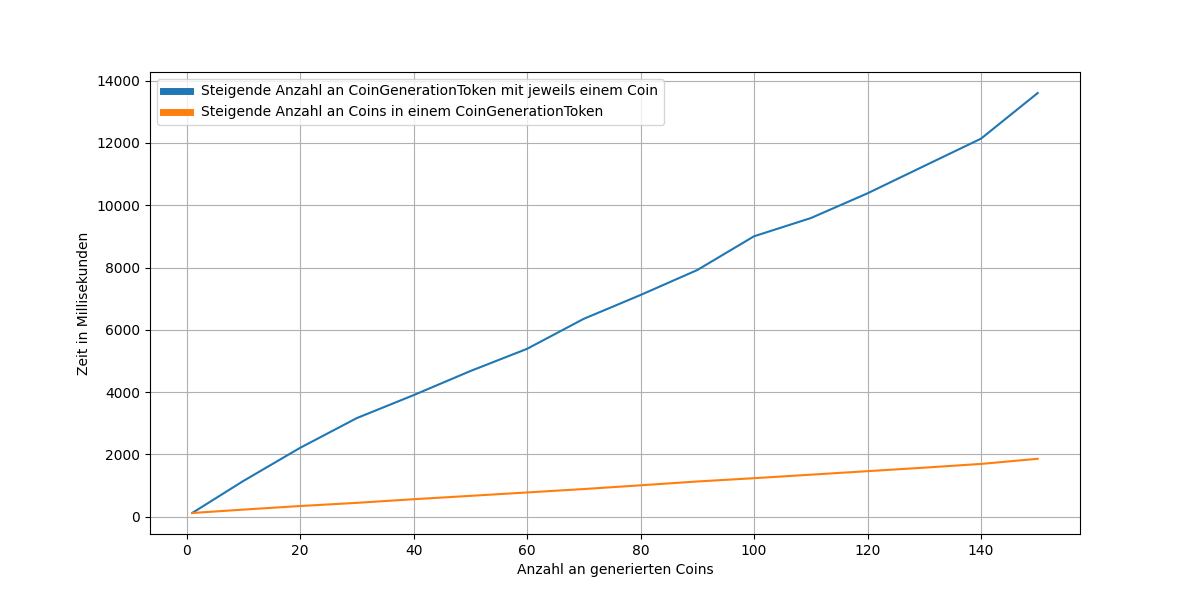
\includegraphics[width=0.8\textwidth]{figure_win_coins.png}
\end{figure}
\begin{figure}[h]
    \caption{Unterschied zwischen steigenden CoinGenerationToken und steigenden Coins innerhalb eines CoinGenerationToken auf MacOS}
    \label{fig:mac_coins}
    \centering
    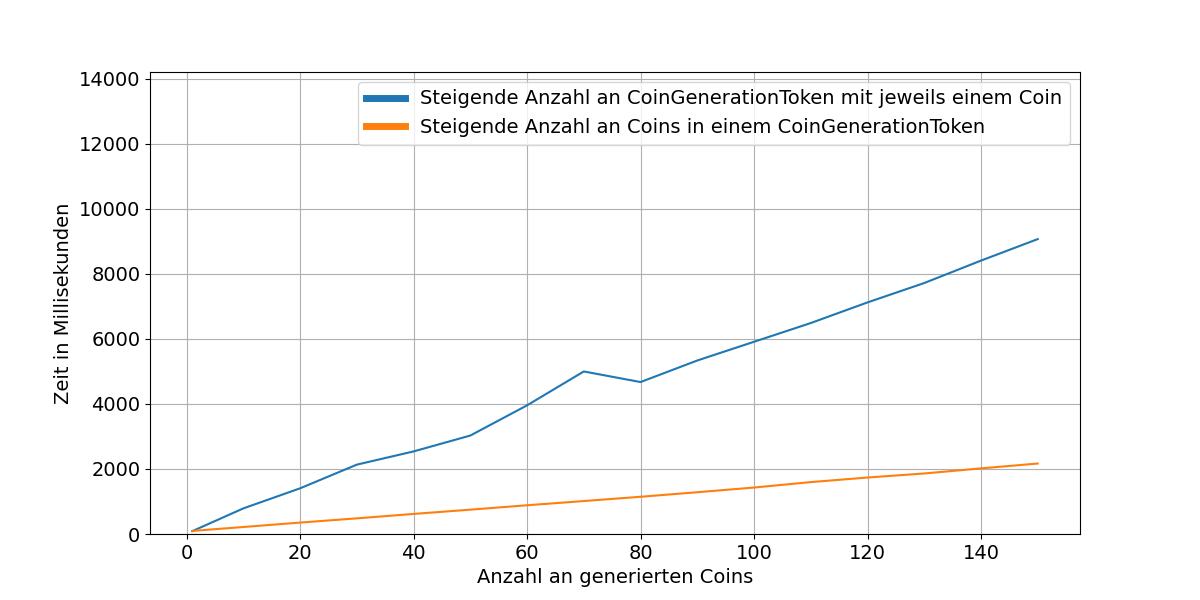
\includegraphics[width=0.8\textwidth]{figure_mac_coins.png}
\end{figure}
Unter direktem Vergleich der Abbildungen \ref{fig:win_coins} und \ref{fig:mac_coins} fällt auf, dass das Erstellen von einem $CoinGenerationToken$ mit 150 Coins erheblich schneller abläuft, als das Erstellen von 150 \\$CoinGenerationToken$ mit jeweils einem Coin. Dies hängt vorallem mit dem anfallenden Mehraufwand in der Verschlüsselung und Datenübertragung zusammen. In Kapitel \ref{system:coingeneration} wird beschrieben, dass für das Erstellen von Coins in der Coin Generierungsphase -- mit Einbezug der partiell blinden Signaturen -- 6 Kommunikationsschritte zwischen dem Exchange und dem Datennutzenden stattfinden. Daraus ergibt sich, dass für das Erstellen und Signieren von 150 Coins innerhalb eines $CoinGenerationTokens$, einen Verbindungsaufbau und 6 Datenübertragungen umfasst, welche jeweils alle mit ECC verschlüsselt sind. Im anderen Fall von 150 $CoinGenerationToken$ entspricht der Aufwand 150 Verbindungsaufbauten sowie 900\todo{Nachrichtenkomplexität verwenden} Datenübertragungen, die mit ECC verschlüsselt sind. Die Nachrichteninhalte die Verschlüsselt werden sind hier dafür nur $\frac{1}{150}$ Mal so groß. Der deutliche Unterschied zwischen den beiden Linien stellt eindeutig dar, welche der beiden Methoden performanter ist.

Deswegen wurde in Abbildungen \ref{fig:win_3} und \ref{fig:win_4} zusätzlich die Anzahl an Coins pro $CoinGenerationToken$ erhöht, da die Auswirkung auf die Gesamtlaufzeit so geringer ist.\\

Beachtlich sind hier vorallem die unterschiedlichen Laufzeiten zwischen der Ausführung auf Windows mit einem AMD Prozessor und der Ausführung auf MacOS mit einem Intel Prozessor. Bei der Ausführung mit 150 $CoinGenerationTokens$ unterscheiden sich die Messwerte beinahe um 50\%. Auf Windows wird dafür eine Gesamtrechendauer von 13696 Millisekunden benötigt, während es auf MacOS lediglich 9277 Millisekunden sind. Gleichzeitig ist das Erstellen von 150 Coins innerhalb eines $CoinGenerationTokens$ auf Windows schneller. Dort wird eine Zeit von 1958 Millisekunden erreicht, während MacOS für die gleichen Opertationen 2389 Millisekunden in anspruch nimmt. Leider kann aufgrund des Aufbaus der beiden Computer nicht bestimmt werden, ob dieser Performanzunterschied durch das Betriebssystem oder durch den Prozessorhersteller entsteht.\\

Die folgende Abbildung \ref{fig:win_3} zeigt das Verhalten der Laufzeiten bei den schrittweisen Anstieg an Datenpostfacheinträgen. Zusätzlich wurden die Anzahl an Coins pro $CoinGenerationToken$ erhöht um ausreichend Coins bereitszustellen. In der Abbildung sind 5 Linien zu sehen. Sie beziehen sich auf unterschiedliche Abschnitte im Protokoll. Die blaue Linie ist die gerade bereits betrachtete Dauer der Coin Generierungsphase. Die orange Linie bildet die Protokollschritte 2,3,4 des in Kapitel \ref{system:payment} dargelegten Bezahlsystem ab. Die Schritte 5,6,7,8,9,10,11 und 12 sind in der grünen Linie mitinbegriffen. Die rote Linie stellt die abschließenden Schritte 13,14,15 und 16 dar.
\begin{figure}[H]
    \caption{Steigende Anzahl an Datenpostfacheinträgen und Coins bei einem CoinGenerationToken und einem Coin pro Bezahlung}
    \label{fig:win_3}
    \centering
    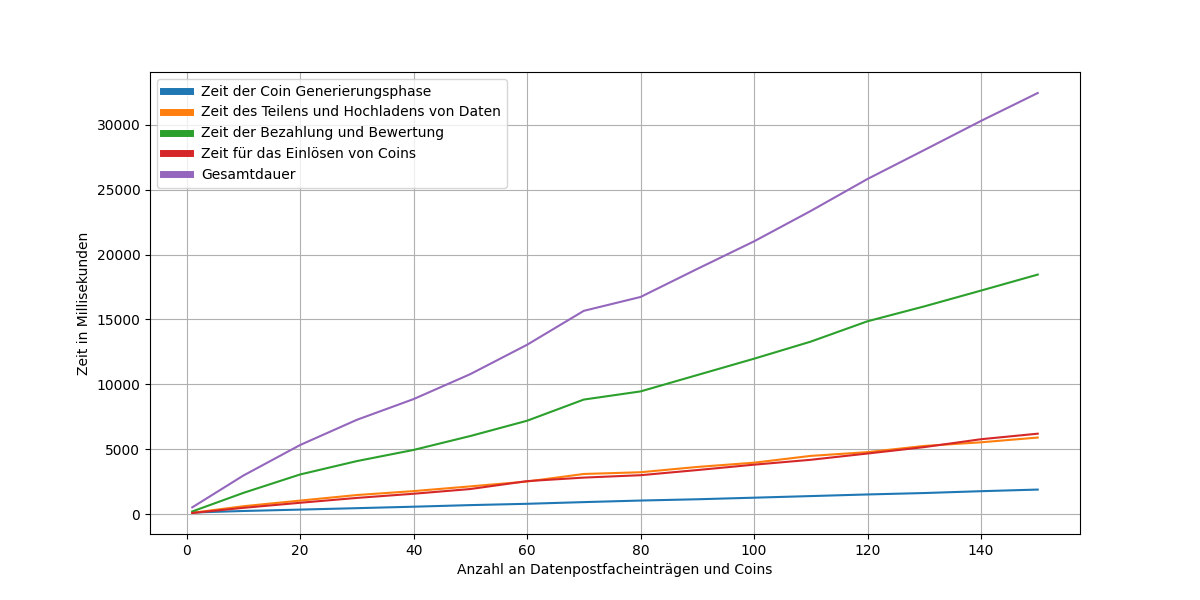
\includegraphics[width=0.8\textwidth]{figure_win_3.png}
\end{figure}
Hier ist zu sehen, dass das Teilen von 150 unterschiedlichen $dataLocations$ und $dataKeys$ in knapp unter 6 Sekunden geschieht. Verglichen mit der Zeit der Bewertung und Bezahlung ist die Zeit passend, da das Anfragen der Aufrufliste ein Mal geschehen muss und nur der Protokollschritt 4 150 Mal ausgeführt. Dieser Schritt verschlüsselt die $dataLocation$, den $dataKey$, den $BewertungsToken$ und den $referenceCode$ symmetrisch mit MAES, was in der Regel schnellere Berechnungszeit liefert als ECC. Nur der Shared-Key wird mit Hilfe von ECC verschlüsselt. 

Bei der Bezahlung und Bewertung hingegen fallen mehrere Schritt an. Hier wird für jeden Datenpostfacheintrag das erhaltene Tupel entschlüsselt, die Reputation angefragt, die Daten angefragt, der Coin zu Bezahlung mit dem $referenceCode$ zurück an das Bezahlpostfach gesendet und der Bewertungstoken zusammen mit einer Bewertung eingereicht. Daher ist ein Anstieg von 5900 Millisekunden auf 18457 Millisekunden beachtlich, da sich die Gesamtanzahl an Operation um ein Fünffaches erhöht. 

Über die Gesamtdauer gesehen wird der erste Computer auch hier wieder um ca 50\% von dem zweiten Computer geschlagen. Dessen Zeiten sind in Abbildung \ref{fig:mac_3} visualisiert und liegen bei 20934 Millisekunden im Gegensatz zu 32447 Millisekunden des ersten Computers. 

\todo{wieder?}Auch hier ist wieder zu beobachten, dass sich alle Zeitmessungen linear zum Anstieg des Parameters verhalten und keine polynomiellen Zeitanstiege zu erkennen sind, welche die Anforderung der Skalierbarkeit verletzten würden.


\begin{figure}[H]
    \caption{Steigende Anzahl an Coins pro Bezahlung und Coins pro CoinGenerationToken bei einem Datenpostfacheintrag und CoinGenerationToken}
    \label{fig:win_4}
    \centering
    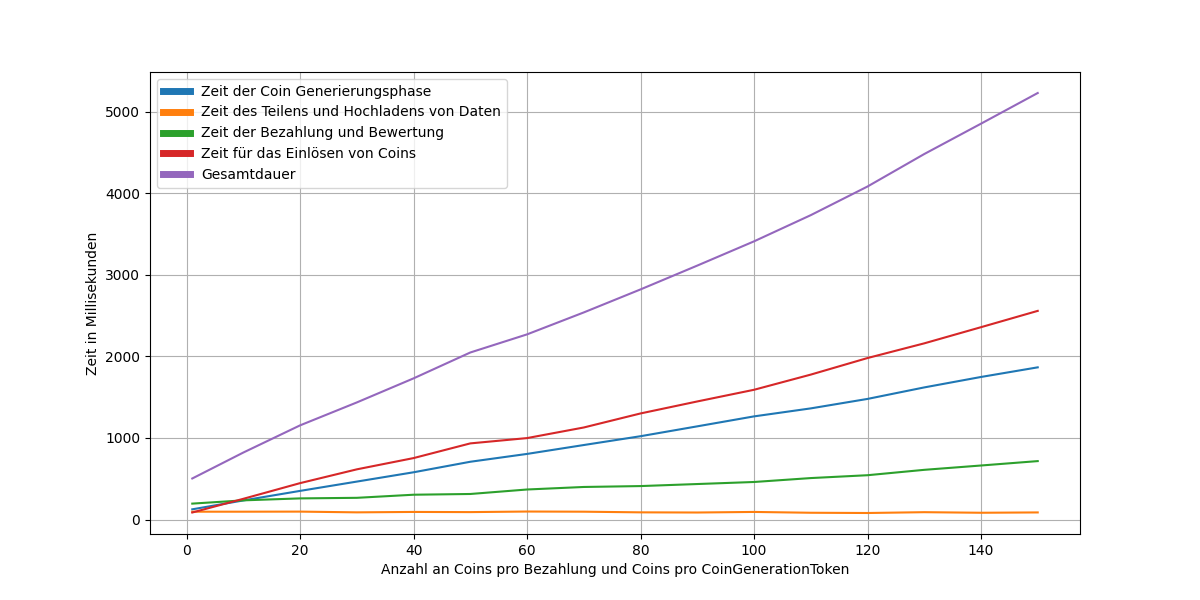
\includegraphics[width=0.8\textwidth]{figure_win_4.png}
\end{figure}
In Abbildung \ref{fig:win_4} wurde nun der vierte Parameter erhöht und so ein Datenpostfacheintrag mit einer steigenden Anzahl an Coins bezahlt. Die Zuteilung der Farben zu den Protokollschritten bleibt hier unverändert zur letzten Abbildung. Es wird sofort deutlich, dass auch hier das Übertragen mehrerer Coins in einer Nachricht erheblich performanter ist, da sich die Gesamtdauer von in Abbildung \ref{fig:win_3} 32447 Millisekunden zu 5227 Millisekunden in Abbildung \ref{fig:win_4} senkt. Diese Abnahme ist wieder durch das Einsparen von hunderten Opertation begründet. Die Protokollschritte 5-12 werden nur noch ein Mal ausgeführt anstatt jeweils 150 Mal. Dadurch sinkt die Zahl an Interaktionen zwischen dem Datentreuhänder und dem Datennutzenden von 1200 auf 8. Im Gegenzug ist die in Schritt 11 verschlüsselte Nachricht, die sämtliche Coins zur Bezahlung beinhaltet, erheblich länger wie bei der Bezahlung mit einem Coin.

Die Dauer für das Einlösen der erhaltenen Coins wird durch die verringerte Anzahl an Postfacheinträgen ebenso gesenkt. Während sie in Abbildung \ref{fig:win_3} noch bei 6198 Millisekunden lag, ist sie in Abbildung \ref{fig:win_4} bereits auf 2557 Millisekunden gefallen. Dies ist hauptsächlich auf den gesparrten Rechenaufwand durch das Entschlüsseln einer einzelnen Nachricht zurückzuführen. Die Zeit zum Erstellen und Absenden eines Datenpostfacheintrags bleibt hier konstant bei ca. 100 Millisekunden, da in jedem Durchlauf genau ein Eintrag erstellt wird und dieser nicht von der Anzahl an Coins beeinflusst wird.


\subsection{Laufzeit ohne Reputation}
Wie in Kapitel \ref{system:reputation} erwähnt wurde, kann das Anfragen der Reputation des Datengebenden sowie das Ausstellen einer Bewertung für die erhaltenen Daten übersprungen werden. Sollte ein Datennutzender keinen großen Wert auf die Qualität der Daten geben oder möchte anderen Datennutzenden keine Einschätzung über die Qualität liefern, so kann er den jeweiligen Schritt weglassen um Rechenaufwand zu sparen. Die Abbildung \ref{fig:win_noRep} zeigt dabei, wie sich das Weglassen der einzelnen Schritte auf die Gesamtlaufzeit auswirkt.
Die unterschiedlich eingefärbten Teile der Balken in der Abbildung \ref{fig:win_noRep} stellen die Laufzeiten der jeweiligen Programmabschnitte dar. Ganz Links ist für die Vergleichbarkeit die Zeit einer Ausführung mit Kontrollparametern zu sehen. Sie umfasst 10 $CoinGenerationToken$ mit jeweils 30 Coins, 100 Datenpostfacheinträge und 3 Coins pro Bezahlung. Diese Werte werden ebenfalls in den kommenden Abschnitten \ref{subsec:runTimeRSA} und \ref{subsec:runTime256Bit} verwendet um eine Kontrollzeit zu definieren. Der Balken in der Mitte verwendet dieselben Werte und zeigt die Dauer der Ausführung, in der das Anfragen der Reputation übersprungen wird. Eine Bewertung wird hier weiterehin abgegeben. Beim rechten Balken wird auch das Einreichen einer Bewertung übersprungen und nur eine Bezahlung abgegeben.\\

\begin{figure}[h]
    \caption{Laufzeitverhalten beim überspringen der Reputationsanfrage und Bewertung}
    \label{fig:win_noRep}
    \centering
    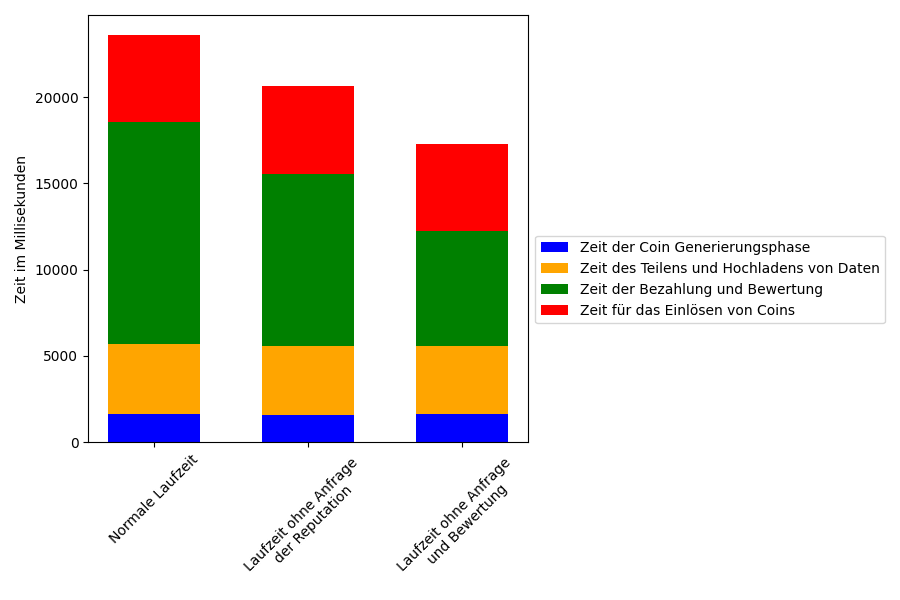
\includegraphics[width=0.8\textwidth]{figure_win_noRep.png}
\end{figure}
In der Abbildung \ref{fig:win_noRep} ist zu erkennen, dass ein moderater Unterschied in der Ausführungsdauer entsteht, sollten die eben angesprochenen Teile des Reputationssystems übersprungen werden. Sämtliche Zeiten der anderen Balkenteile unterscheiden sich nur in Messungenauigkeiten. Durch das Entfallen der Reputationsanfrage werden bereits zwei Protokollschritte übersprungen, was auf die Menge an Ausführungen hochgerechnet, 200 Nachrichten entspricht. Der dadurch gewonnene Zeitunterschied umfasst 2956 Millisekunden. Beim zusätzlichen weglassen der Bewertung werden weitere 100 Nachrichten gesparrt. Da diese Nachrichten den Bewertungstoken enthalten muss der Datentreuhänder beim Empfang die -- in Kapitel \ref{system:reputation} genannte -- Überprüfung vornehmen. Diese Überprüfungen bleiben beim Weglassen einer Bewertung aus, was die Laufzeit um weitere 3334 Millisekunden verkürzt. Für Datennutzende mit wenig Rechenleistung ist es daher eine Überlegung wert, von dem vorgesehenen Protokoll etwas abzuweichen und die Anfrage der Reputation beispielsweise nur bei schlechten Daten durchzuführen, um zu prüfen, ob es sich um einen Betrugsversuch handelt.
\subsection{Laufzeit mit 256 Bit Security Level}
\label{subsec:runTime256Bit}
In dem Kapitel \ref{chap:impl} wurde beschrieben, dass sich für die Einhaltung eines 128 Bit Security Level entschieden wurde und die Gründe dafür genannt. Der größte Nachteil ist der Anstieg der Rechenzeit, den größere Schlüssellängen mit sich ziehen. Um genau zu bewerten wie groß der dadurch entstehende Unterschied ist, wird in der Abbildung \ref{fig:win_256bit} ein Durchlauf mit Kontrollausführungszeit -- wie oben beschrieben -- gegen einen Durchlauf mit einem 256 Bit Security Level verglichen.
Das Security Bit Level von 256 Bits kann leider nicht ganz erreicht werden. In Abschnitt \ref{sec:aes} wird der MAES Algorithmus erklärt. Dieser ist aufgrund seines Konzeptes an einen 128 Bit langen Schlüssel gebunden und kann daher nicht auf 256 Bit erweitert werden. Ansonsten wurde für ECC die $secp521r1$ Kurven verwendet, die 256 Bit Sicherheit liefert \cite{ecc-duka2020elliptic}, sowie die Parameter für die partiell blinden Signaturen auf -- für 256 Bit Security übliche -- Werte angehoben. Diese entsprechen $L=15360$ und $N=512$ \cite{elaine2016recommendation}.

Die Abbildung \ref{fig:win_256bit} zeigt die gemessenen Zeitunterschiede bei der Verwendung von 256 Bit Security Parametern. Nicht in der Abbildung aufgeführt sind die benötigten Zeiten zum Erstellen der Schlüssel, da diese beim Starten der Applikation generiert werden und daher nicht in die Berechnungszeit von Aktionen einfließen. Diese werden zu Beginn einmal erstellt. Jedoch sind sie nicht zu vernachlässigen. Bei ECC ist der Unterschied beim Generieren eines Schlüssels vergleichsweise gering. Die Kurven $secp256k1$ und $secp521r1$ unterscheiden sich hierbei um circa 10 Millisekunden \cite{ecc-duka2020elliptic}. Das Generieren von Parametern der partiell blinden Signaturen hingegen unterscheidet sich in der eigenen Implementation signierfikant. Für den Vergleich wurde die Zeit der Generierung für 128 Bit und 256 Bit jeweils 10 Mal gestoppt. Die Werte für 128 Bit lagen zwischen 95 - 6737 Millisekunden mit einem Durchschnitt von 1760 Millisekunden. Bei 256 Bit hingegen lagen die Werte zwischen 6556-102644 Millisekunden mit einen Durchschnitt von 38022 Millisekunden. Hier ist der Unterschied zwischen den Security Level deutlich erkennbar.

\begin{figure}[h]
    \caption{Laufzeitverhalten unter Einsetzung eines 256 Bit Security Levels}
    \label{fig:win_256bit}
    \centering
    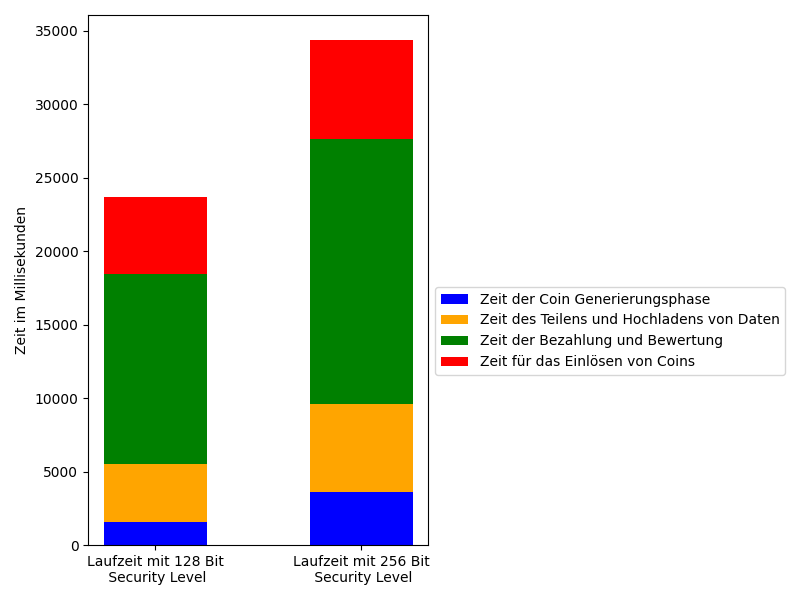
\includegraphics[width=0.8\textwidth]{figure_win_256Bit.png}
\end{figure}
Die Zeitunterschiede die durch das Verschlüsseln sowie Signieren von Nachrichten entstehen sind in Abbilung \ref{fig:win_256bit} dargestellt. Für die Werterhebung wurde jeweils ein Durchlauf mit den Kontrollparametern für 128 Bit auf der linken Seiten und 256 Bit auf der rechten Seite ausgeführt. Hier sind die unterschiedlichen Laufzeiten gut zu erkennen. Die Gesamtausführungszeit steigt um beinahe die Hälfte, von 23713 Millisekunden auf 34372 Millisekunden. Da alle Schritte der Protokolle die Daten verschlüsselt übertragen, sind Anstiege in alle Bereichen zu verzeichnen. Am größten sind die Unterschiede in der Coin Generierungsphase. Hier wächst die gemessene Zeit um mehr als das Doppelte, von 1591 Millisekunden auf 3624 Millisekunden. Dies hängt mit der Anwendung der partiell blinden Signatur zusammen, welche durch den jetzt fünffach so langen Schlüssel, vergleichsweise mehr Zeit in Anspruch nimmt, als das Verschlüsseln mit einem doppelt so langen Schlüssel bei ECC. Das Erstellen und Hochladen der 30 Datenpostfacheinträge verzögert sich um 2079 Millisekunden und liegt unter Verwendung von 256 Bit bei insgesamt 5977 Millisekunden. Die Steigerung liegt hier -- genauso wie bei der Zeit zum Bezahlen und Bewerten -- bei knapp 50\%. Die Zeit zum Bezahlen steigt von 12999 Millisekunden auf 18036 Millisekunden. Erstaunlicherweise verlängert sich die Zeit zum Einlösen der Coins am geringsten. Der gemessene Anstieg beträgt hier lediglich 1509 Millisekunden, was in etwa 30\% entspricht. Anhand der Coin Generationphase wurde erwartet, dass sich die Zeit zum Einlösen ähnlich stark verlängern wird. Allerdings scheint dieser Abschnitt des Protokolls durch die Auswirkungen der verlängerten Schlüssel am wenigsten betroffen zu sein.

\subsection{Laufzeit mit RSA}
\label{subsec:runTimeRSA}
In Abschnitt \ref{sec:ecc} wird erklärt, dass die elliptische Kurven Kryptographie große Unterschiede in der Laufzeit im Vergleich zu RSA erzielen kann. Für eine Bewertung des Zeitaufwands der durch die Verwendung von ECC gewonnen wird, wurden sämtliche ECC Kommunikationsverschlüsselungen durch RSA ersetzt und die Zeit einer Ausführung gemessen. Für die RSA Schlüssel wurde ein Länge von 3072 Bit verwendet, wie sie in der Literatur für ein Security Bit Level von 128 Bit empfohlen wird \cite{elaine2016recommendation}. Die daraus entstandenen Ergebnisse sind in Abbilung \ref{fig:win_rsa} zu sehen. Sie zeigen die Ausführung mit den Kontrollparametern, unter Verwendung von ECC auf der linken Seite und Verwendung von RSA in der Mitte sowie auf der rechten Seiten. Auf der rechten Seite wird für jeden Postfacheintrag ein neues Schlüsselpaar erstellt, wie es im Protokoll (Kapitel \ref{system:payment} Schritt 4)\todo{is it though?} vprgeben ist. Dieser Schritt wurde in der Mitte ausgelassen, um die reinen Unterschiede der Verschlüsselungsdauer zu beurteilen.

\begin{figure}[h]
    \caption{Laufzeitverhalten unter Verwendung von RSA für Verschlüsselung}
    \label{fig:win_rsa}
    \centering
    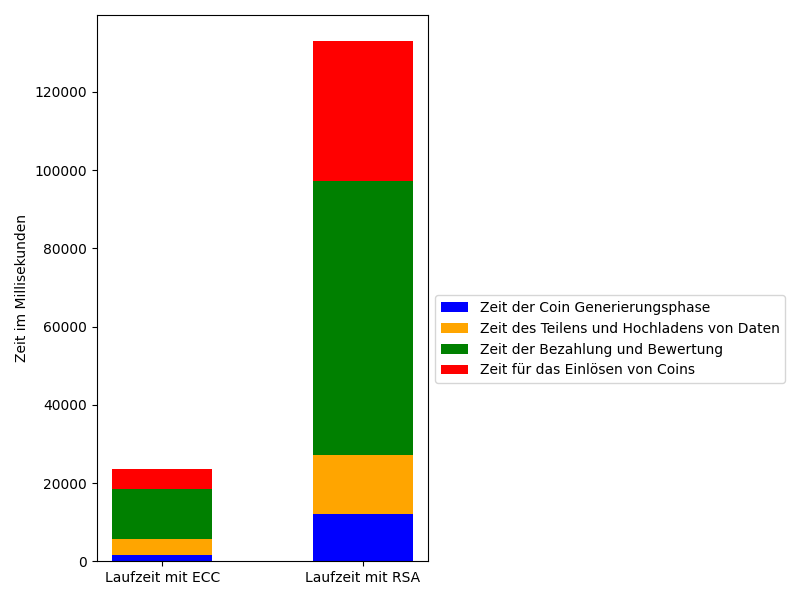
\includegraphics[width=0.8\textwidth]{figure_win_RSA.png}
\end{figure}
Die hier entstehenden Unterschiede sind maßgeblich und deutlich erkennbar. ECC schlägt RSA -- ohne neue Schlüsselgenerierung -- bei der Gesamtlaufzeit um den Faktor fünf. Dabei werden vorallem die Zeiten der Coin Generierungsphase sowie Coin Einlösephase langsamer als die anderen Protokollschritte. Sie steigen um die Faktoren $7,3$ und $7,1$, während sich die Zeiten für das Hochladen der Datenpostfacheinträge und das Bezahlen und Bewerten um die Faktoren $3,7$ und $5,4$ erhöht. Bei Vergleich der Laufzeit mit neuer Schlüsselgenerierung werden die in Abschnitt \ref{subsec:runTime256Bit} genannten Unterschiede der Laufzeiten zwischen ECC und RSA deutlich. Die Differenz zwischen den Zeiten des Datenpostfacheintrags Erstellen, zwischen dem mittleren und rechten Balken, berufen sich auf 340.000 Millisekunden, was in etwa 3400 Millisekunden für das Erstellen eines Schlüsselpaars bedeutet.

Anhand der Abbildung \ref{fig:win_rsa} ist eindeutig zu sehen, dass die Verwendung von ECC als Verschlüsselungsmethode immense Laufzeitunterschiede liefert. Zusammen mit der neuen Schlüsselgenerierung für jeden Postfacheintrag ergibt sich für ECC eine Laufzeit, die $21,16$ Mal schneller ist wie die gleichen Opertationen mit RSA. Daher wird die Verwendung von ECC hier eindeutig vor RSA bevorzugt.\\

Abschließend kann zusammengefasst werden, dass sich die Rechendauer der vier verschiedenen Protokollabschnitte mit einer steigenden Anzahl an Eingaben linear verhält. Zwar laufen einige Abschnitte schneller als andere, wie beispielsweise das Erstellen von Coins durch einen $CoinGenerationToken$ anstatt durch mehrere, was sich selbst von Computer zu Computer unterschiedlich verhalten kann. Allerdings wird zu keinem Zeitpunkt ein polynomielles Laufzeitverhalten beobachtet. Das Überspringen von Reputationsanfragen wie das Prüfen der Reputation oder das Einreichen einer Bewertung, ist in bestimmten Situationen möglich und liefert dabei Laufzeiteinsparungen von bis zu über 6 Sekunden. Daher können Strategien entwickelt werden um die Verwendung dieser Anfragen zu minimieren und so den Rechenaufwand zu verringern. Insbesondere für Datennutzende, die nur über eingeschränkte Rechenleistung verfügen, sind solche Möglichkeit in Betracht zu ziehen. Ein Security Bit Level von 128 Bit ist laut Literatur auch für die kommenden Jahre mehr als ausreichend \cite{elaine2016recommendation,bsi2020cryptographic}. Während der Umstieg auf ein Security Bit Level von 256 Bits in anbetracht der sensiblen kommunizierten Daten nachvollziehbar wäre, zieht dieser einen zusätzlichen Rechenaufwand mit sich. Die dadurch hinzukommende Steigerung von fast 50\% ist nicht zuvernachlässigen. Aufgrund dessen wird für die Verwendung des Systems ein Security Bit Level von 128 Bit empfohlen. Anhand der in Abbildung \ref{fig:win_rsa} visualisierten Performanzunterschiede zwischen ECC und RSA wird hier eindeutig ECC für die Verschlüsselung und Schlüsselgenerierung empfohlen, da es RSA um mehr als ein Zwanzigfaches überholt.

\section{Erfüllen der Anforderungen}
In diesem Abschnitt wird kurz gezeigt, dass alle der in Kapitel \ref{chap:req} gesetzten Anforderungen durch das hier präsentierte Konzept erfüllt werden.

\paragraph{Funktionale Anforderungen.}
\begin{enumerate}
    \item Die Präsenz eines Bezahlsystems ist eindeutig. Durch die Coin Generationphase wird zusammen mit den Protokollschritten 11,14,15,17 des Bezahlsystems aus Kapitel \ref{system:payment} ein Austausch von Zahlungsmittel möglich welcher dem Datengebenden für seine Daten entlohnt.
    \item Es existiert ein Reputationswert. Dieser ist zwar nicht anhand der Daten definiert sondern des Datengebenden, allerdings wird durch die Angabe des Reputationsschwellwert beim Erstellen eines Aufrufs sichergestellt, dass ein Datennutzender eine gewisse Qualität vorraussetzen kann.
    \item Die Streitfälle Fehlerhafte Coins sowie Bezahlzeitraum überschritten sorgen dafür, dass ein Datengebender bei rechtmäßiger Bereitstellung seiner Daten eine Bezahlung erhält. Der Shared-Key kann dabei verwendet werden um die Übertragung der Coins zu beweisen.
    \item Der Bewertungstoken der Teil des Datenpostfacheintrags ist, liefert dem Datennutzenden die Möglichkeit eine Bewertung der Daten an den Datentreuhänder zu senden, ohne dabei die Identität des Datengebenden zu kennen.
    \item Sollte ein Datengebender versuchen eine Bewertung seiner Daten zu verhindern, so greifen die Streitfälle Kein/Doppleter Bewertungstoken oder Inkorrekte Signatur die den Datengebenden bestrafen.
    \item Durch den $nonce$ der Teil des Bewertungstokens ist, wird sichergestellt, dass ein Datennutzender nur eine Bewertung pro Token und damit auch pro Handel abgeben kann.
\end{enumerate} 

\paragraph{Nicht funktionale Anforderung}
\begin{enumerate}
    \item Die Betrachtung der Angreifermodelle aus den Abschnitten \ref{subsec:adversaryCoinGen}, \ref{subsec:adversaryPayment} und \ref{subsec:adversaryRep} zeigen, dass der Datengebende und dessen Verhalten zu keinem Zeitpunkt des Protokolls bestimmt werden können. Er bleibt daher anonym.
    \item Die Unverkettbarkeit wird ebenfalls in den Angreifermodellen gezeigt. Durch die Funktionsweise bleiben sowohl verschiedene Handel eines Datengebenden als auch die Beziehung zwischen Datengebenden und Datennutzenden unverkettbar.
    \item In dem Abschnitt \ref{sec:computationTime} wird gezeigt, dass das eine Transkationen von Daten im Tausch für Coins sowie das Einlösen dieser Coins in unter einer Sekunde abläuft, was in diesem Kontext -- vorallem verglichen mit alternativen wie Bitcoin -- vernachlässigbar ist.
    \item Abschnitt \ref{sec:computationTime} zeigt zusätzlich, dass der Rechenaufwand mit steigender Anzahl an Transkationen linear steigt.
    \item Dass das System die Vertraulichkeit und Integrität der Daten und Coins beim Austausch dieser schützt wird in Abschnitt \ref{sec:auswertungSecurity} dargelegt.
\end{enumerate}

Es sind also sowohl alle funktionalen als auch nicht funktionalen Anforderungen an das System erfüllt.

\section{Wie kann ein privatsphäreschützender Anreiz zur Benutzung eines Datentreuhändermodells geschaffen werden?}

\section{Wie kann dieser Anreiz gegen Missbrauch geschützt werden?}

\section{Diskussion}
\label{sec:discussion}
In diesem Abschnitt werden einige noch offene Punkte genannt, die bei der Entwicklung der Konzepte entstanden, aber noch nicht umgesetzt werden konnten. 

Der erste Punkt ist der saubere Umsetzung der Qualitätsbewertung durch den Datentreuhänder. In Kapitel \ref{sec:dt} wird beschrieben, dass manche Datentreuhänder Mechanismen zur Qualitätssicherung besitzen. Sollte das System jedoch in einem Datentreuhändersystem implementiert werden, der nicht über solch einen Mechanismus verfügt, kann die Qualität nicht bewertet werden, was eine große Angriffsmöglichkeit für bösartige Datengebende schafft. Zusätzlich werden bei der Schlichtung eines Streitfalls viele Informationen für den Datentreuhänder einsehbar. All diese Informationen sind zum Schlichten des Streitfalls erforderlich, weshalb sie nicht privat gehalten werden können. Trotzdem kann ein Ziel von zukünftigen Arbeiten sein, die Menge an Informationen die beim Schlichten eines Streitfalls preisgegeben werden zu minimieren.

Der nächste Punkt ist die Verwendung des Datennutzenden Zertifikats. Es liefert eine große Schwachstelle, sollte ein Datennutzender sein Zertifikat öffentlich macht. Da es keine Informationen über den Datennutzenden beinhaltet, könnte ein Datengebender der in Besitz eines solchen Zertifikates gelangt, sich selbst Bewertungen ausstellen. Deswegen sollte -- bevor das System produktiv eingesetzt wird -- die Verwendung des Zertifikates durch eine andere Art von Zero Knowledge Proof ersetzt werden. Dieser Schritt wurde hier aus zeitlichen Gründen noch nicht getätigt.

Zuletzt war lange Zeit ein alternativer Ansatz für die Umsetzung des Reputationssystems angedacht. Hier wird begründet, warum der aktuelle Ansatz diesem bevorzugt wird. Der alternative Ansatz basiert auf einem Beweis von erhaltenen Coins. Hier wird beim Einlösen von Coins durch den Exchange ein Zertifikat ausgestellt, dass belegt, dass der Datengebende erfolgreich eine Summe an Coins eingelöst hat. Dieses Zertifikat kann anstatt des Reputationswertes dem Datennutzenden vorgelegt werden, um den Ruf eines Datengebende zu zeigen. Da ein hoher Betrag eines Datengebenden von einer langen erfolgreichen Benutzung des Datentreuhänder zeugt, kann Datengebenden mit hoher Summe mehr vertraut werden. Dieser Ansatz hat jedoch zwei Schwachstelle, die ihn benachteiligen. Zuerst kann solch ein Zertifikat leicht gestohlen werden. Da es keine Informationen über der Inhaber enthalten darf -- da sonst die Anonymität des Datengebenden gegenüber des Datennutzenden nicht mehr gewährleistet ist -- kann es durch einen Dieb als sein eigenes Zertifikat verwendet werden. Des Weiteren wird ein Datengebender mit hohem Betrag auf seinem Zertifikat nicht mehr dazu angereizt qualitativ hochweritge Daten zu liefern. Da sich die Menge der erhaltenen Coins nicht verkleinern kann, kann er konstant qualitativ schlechte Daten verkaufen ohne das dies Auswirkungen auf seinen Ruf hat. Aus diesen Gründen wurde sich für eine reputationswertbasierte Variante entschieden.
% Lösen des Streitfalls legt viele Daten offen
% DN Zertifikat durch ZKP ersetzen
% alternatives rating system mit Kontostand beschreiben und nachteile nennen


% länge des ciphertext lässt schließen wie viele coins übertragen werden

%==================================================================================================


\chapter{Zusammenfassung}


%==================================================================================================



\thispagestyle{empty}

\vspace*{\fill}
\pagestyle{empty}

{
    \normalsize
    \begin{center}
        \textbf{Eidesstattliche Erklärung}
    \end{center}
    Hiermit versichere ich an Eides statt, dass ich die vorliegende Arbeit im Bachelorstudiengang Software-System-Entwicklung
    selbstständig verfasst und keine anderen als die angegebenen Hilfsmittel –- insbesondere keine im Quellenverzeichnis nicht benannten Internet-Quellen –- benutzt habe. Alle Stellen, die wörtlich oder sinngemäß aus Veröffentlichungen entnommen wurden, sind als solche kenntlich gemacht. Ich versichere weiterhin, dass ich die Arbeit vorher nicht in einem anderen Prüfungsverfahren eingereicht habe.
    \vspace*{1cm}\\
    Hamburg, den \today
    \hspace*{\fill}\begin{tabular}{@{}l@{}}\hline
    \makebox[5cm]{Knut Hoffmeister}
    \end{tabular}
    \vspace*{3cm}
}
\vspace*{\fill}

\printbibliography

\appendix 
\chapter{Laufzeit Abbildungen}
\begin{figure}[H]
    \caption{Mac 1}
    \centering
    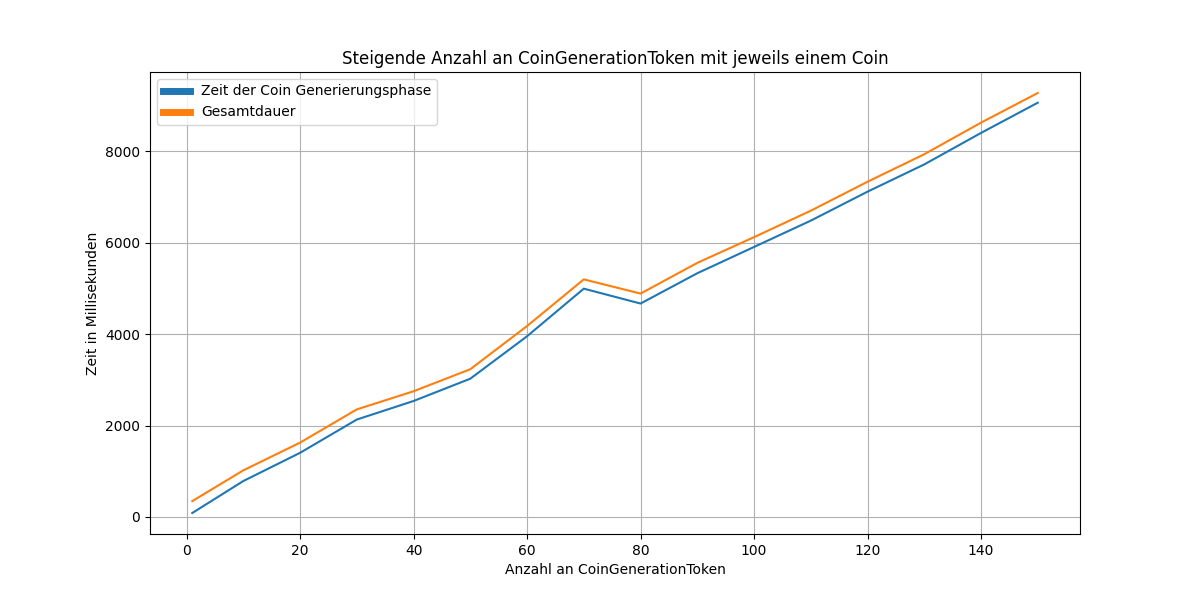
\includegraphics[width=0.8\textwidth]{figure_mac_1.png}
    \label{fig:mac_1}
\end{figure}
\begin{figure}[H]
    \caption{Mac 2}
    \centering
    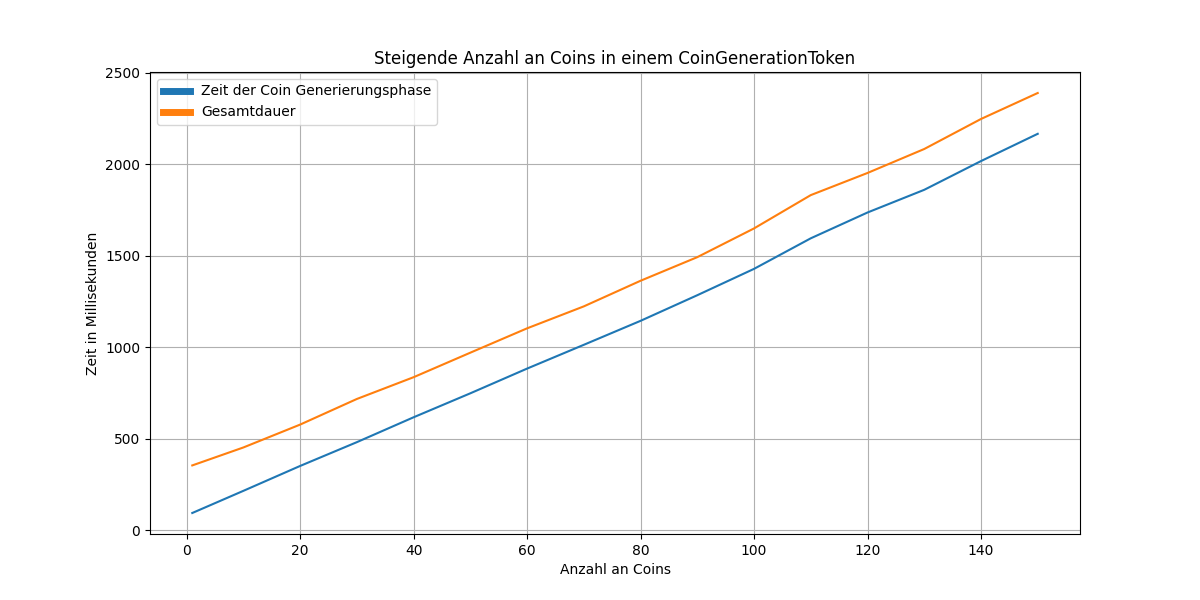
\includegraphics[width=0.8\textwidth]{figure_mac_2.png}
    \label{fig:mac_2}
\end{figure}
\begin{figure}[H]
    \caption{Mac 3}
    \centering
    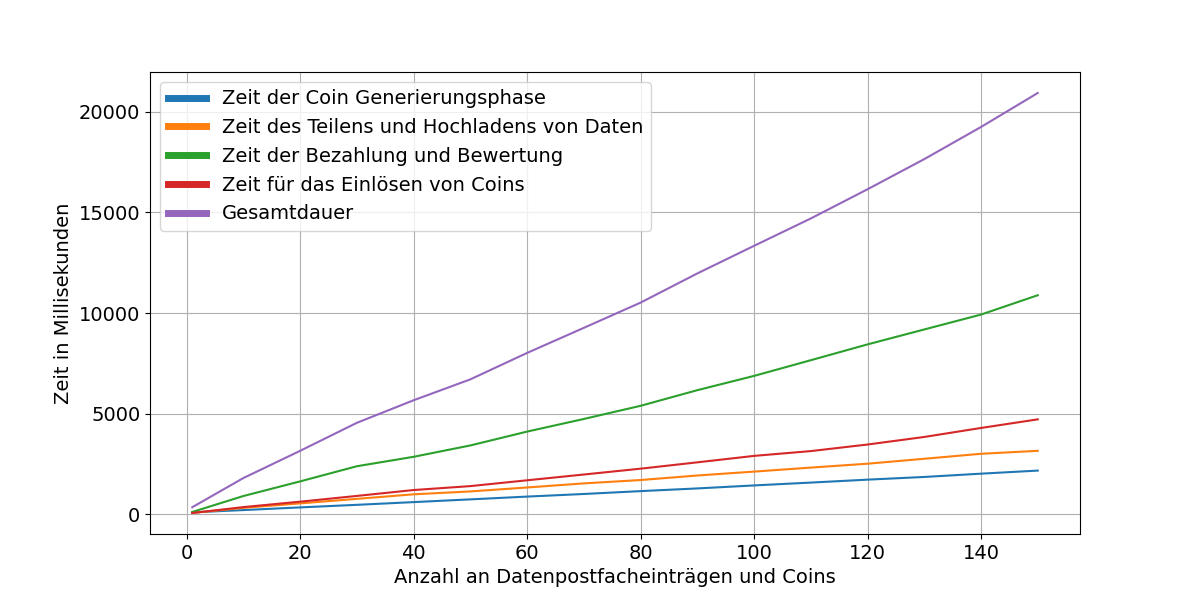
\includegraphics[width=0.8\textwidth]{figure_mac_3.png}
    \label{fig:mac_3}
\end{figure}
\begin{figure}[H]
    \caption{Mac 4}
    \centering
    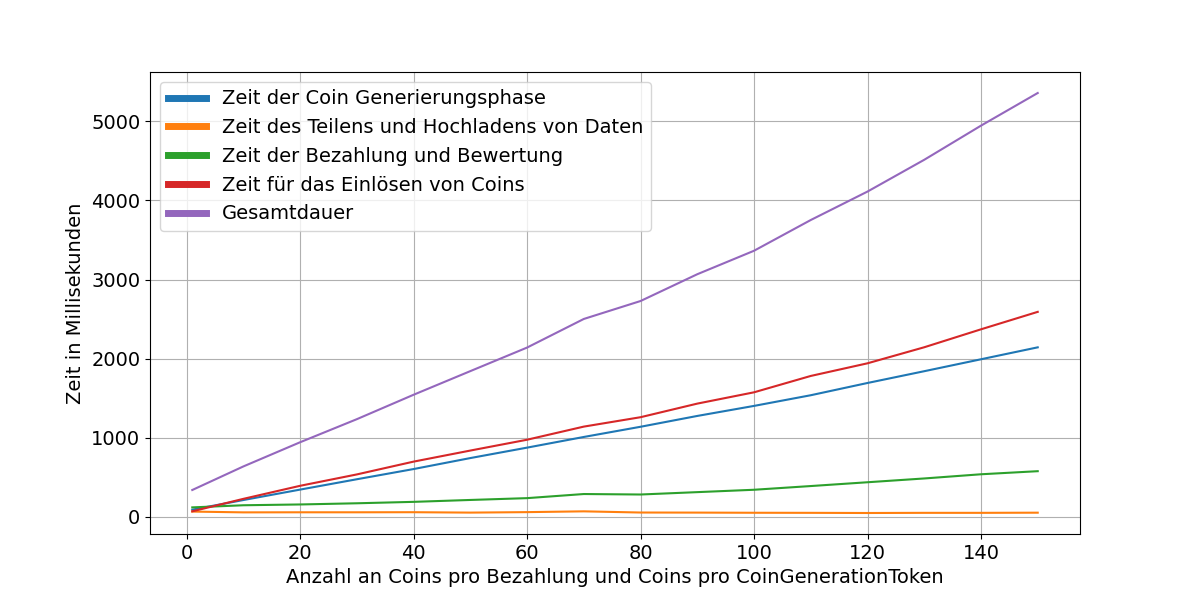
\includegraphics[width=0.8\textwidth]{figure_mac_4.png}
    \label{fig:mac_4}
\end{figure}
\end{document}